\documentclass[12pt]{article}
\usepackage[utf8]{inputenc}
\usepackage[spanish]{babel}
\usepackage{graphicx}
\usepackage{geometry}
\usepackage{caption}
\usepackage{subcaption}
\usepackage{float}

\geometry{margin=1in}

\title{Práctica de Laboratorio: Muestreo, Retención y Transmisión}
\author{Estudiante de Comunicaciones}
\date{\today}

\begin{document}

\section{Procedimiento y Resultados}

\subsection{Paso 3: Reloj Universal}
\textbf{Instrucciones:} Observe las diferentes señales de reloj presentes en la tarjeta, determine sus frecuencias y las relaciones entre ellas. Seleccione la menor de ellas como señal de muestreo. Especifique las características de las señales que con este reloj se pueden muestrear. Explique.

% \begin{figure}[H]
%     \centering
%     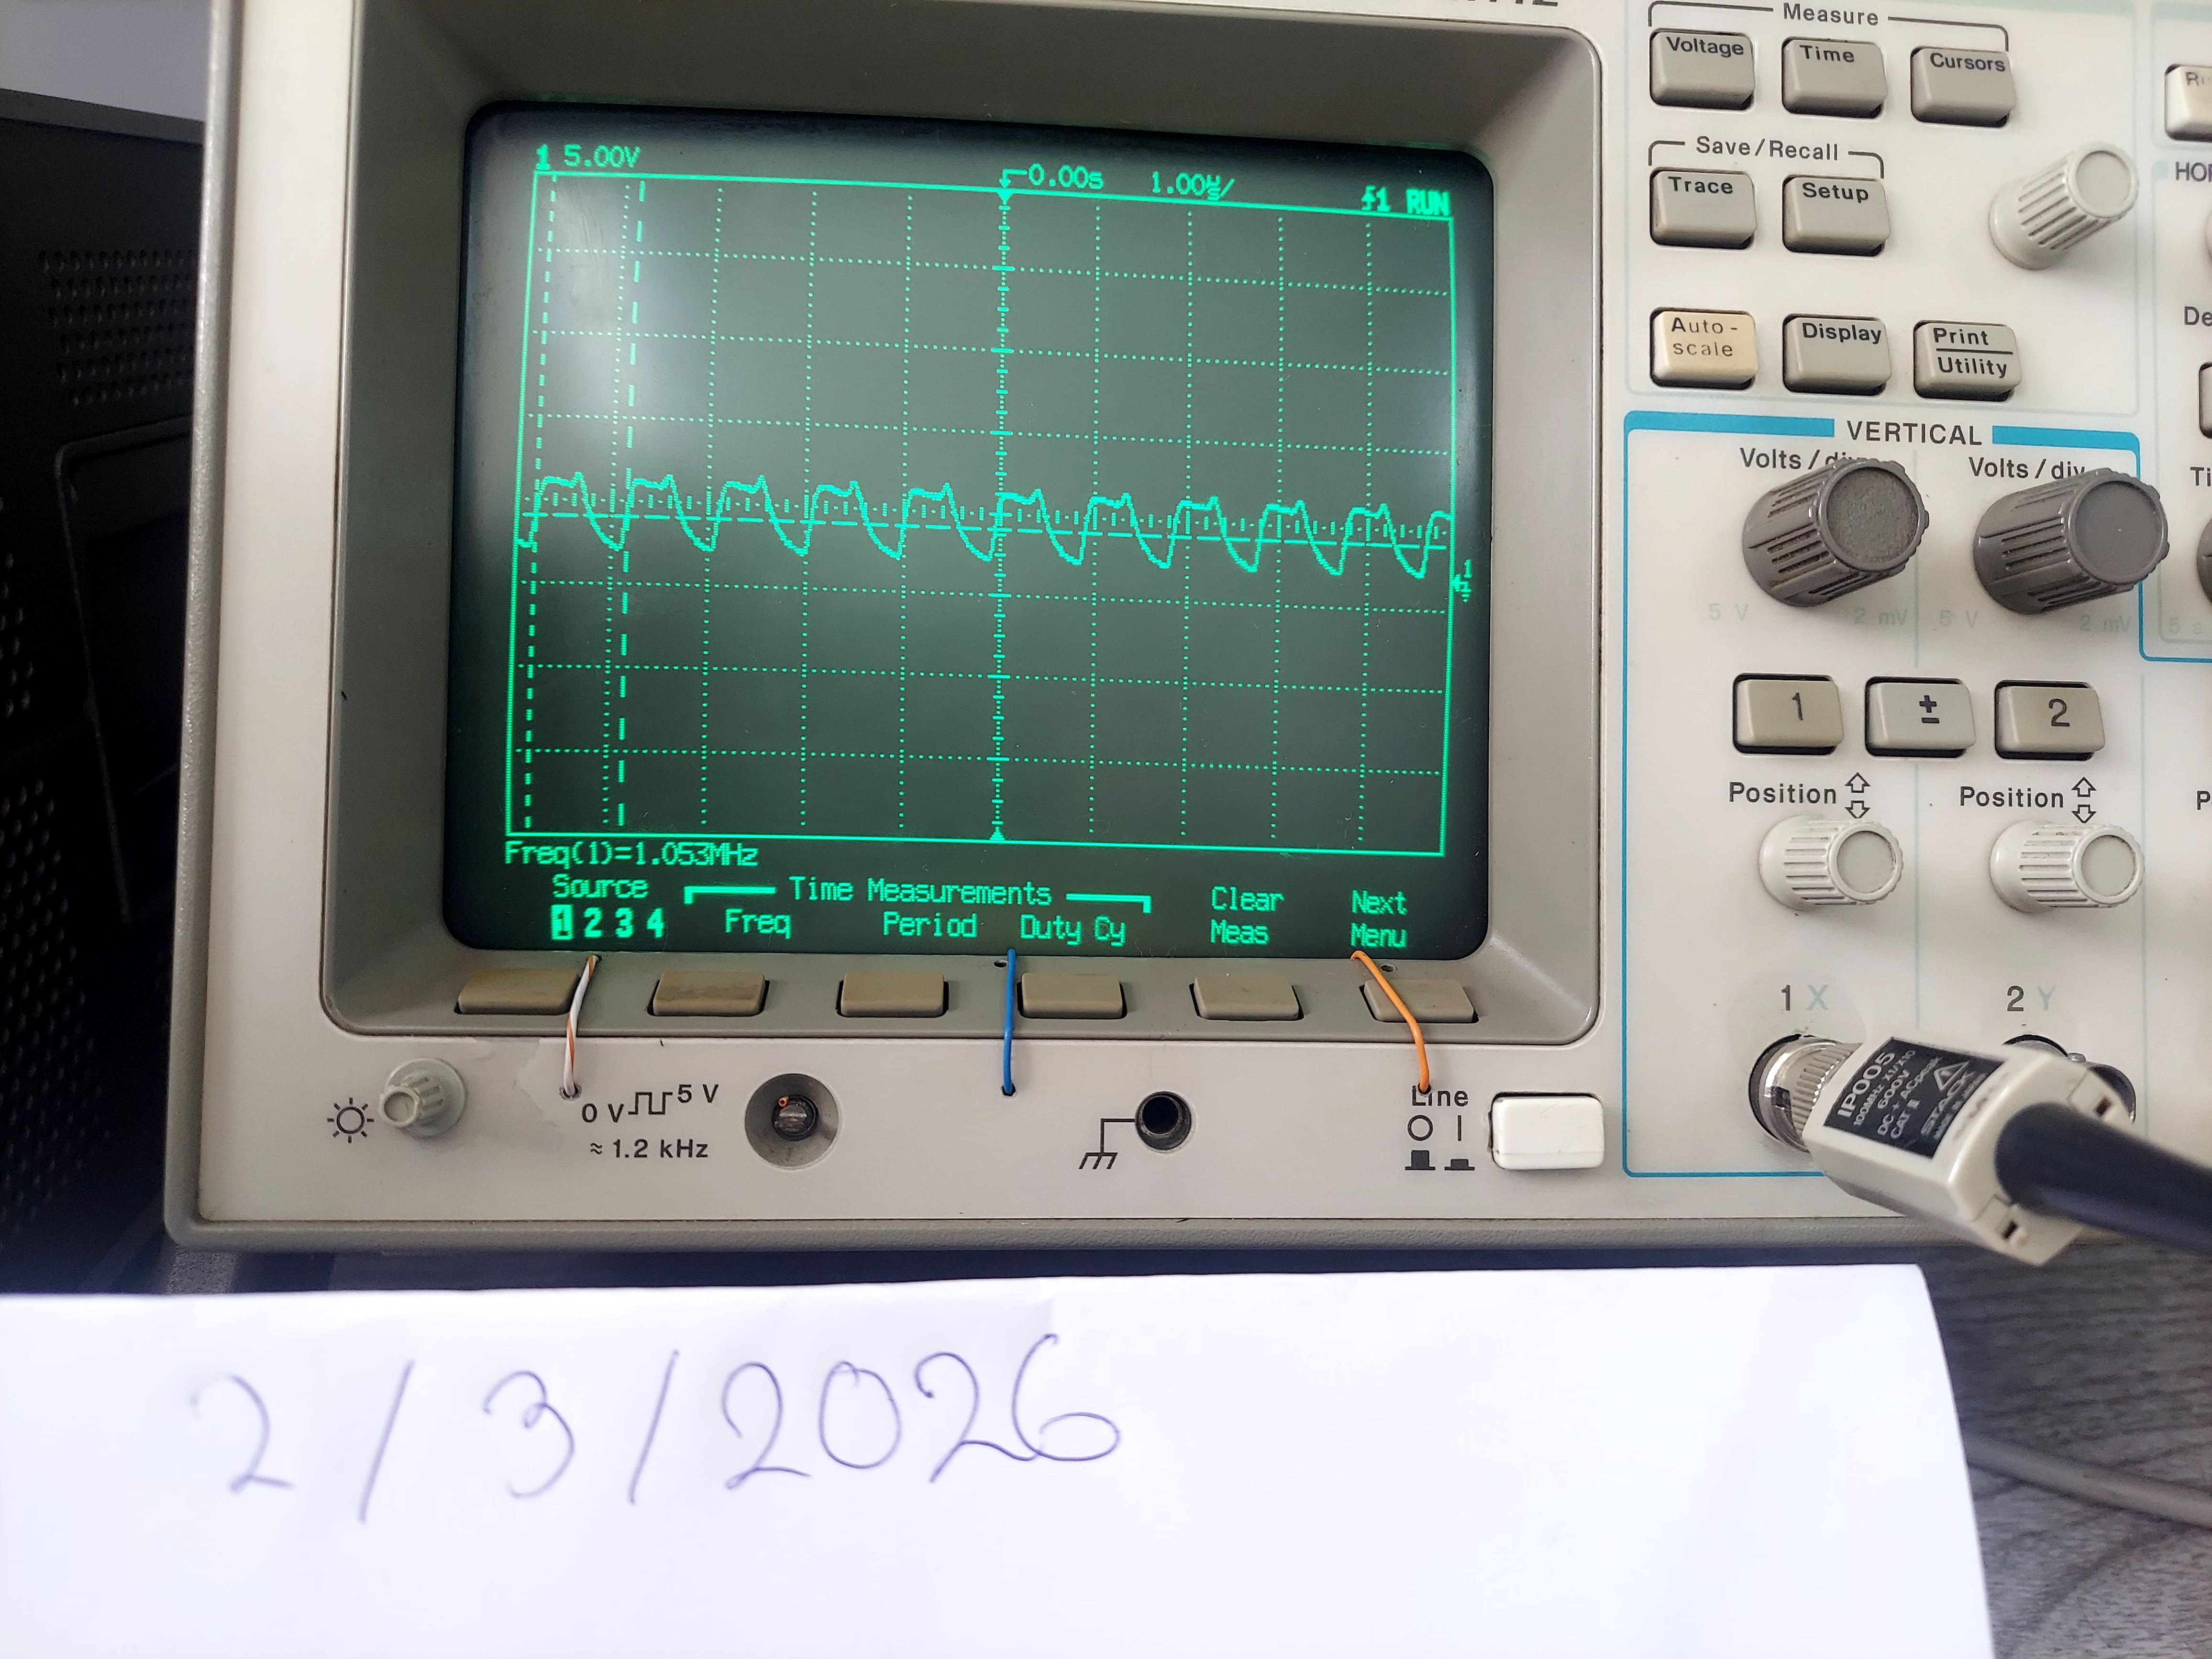
\includegraphics[width=0.8\textwidth]{Imagenes/3-reloj-universal-a.jpg}
%     \caption{Señal de reloj A}
% \end{figure}

% \begin{figure}[H]
%     \centering
%     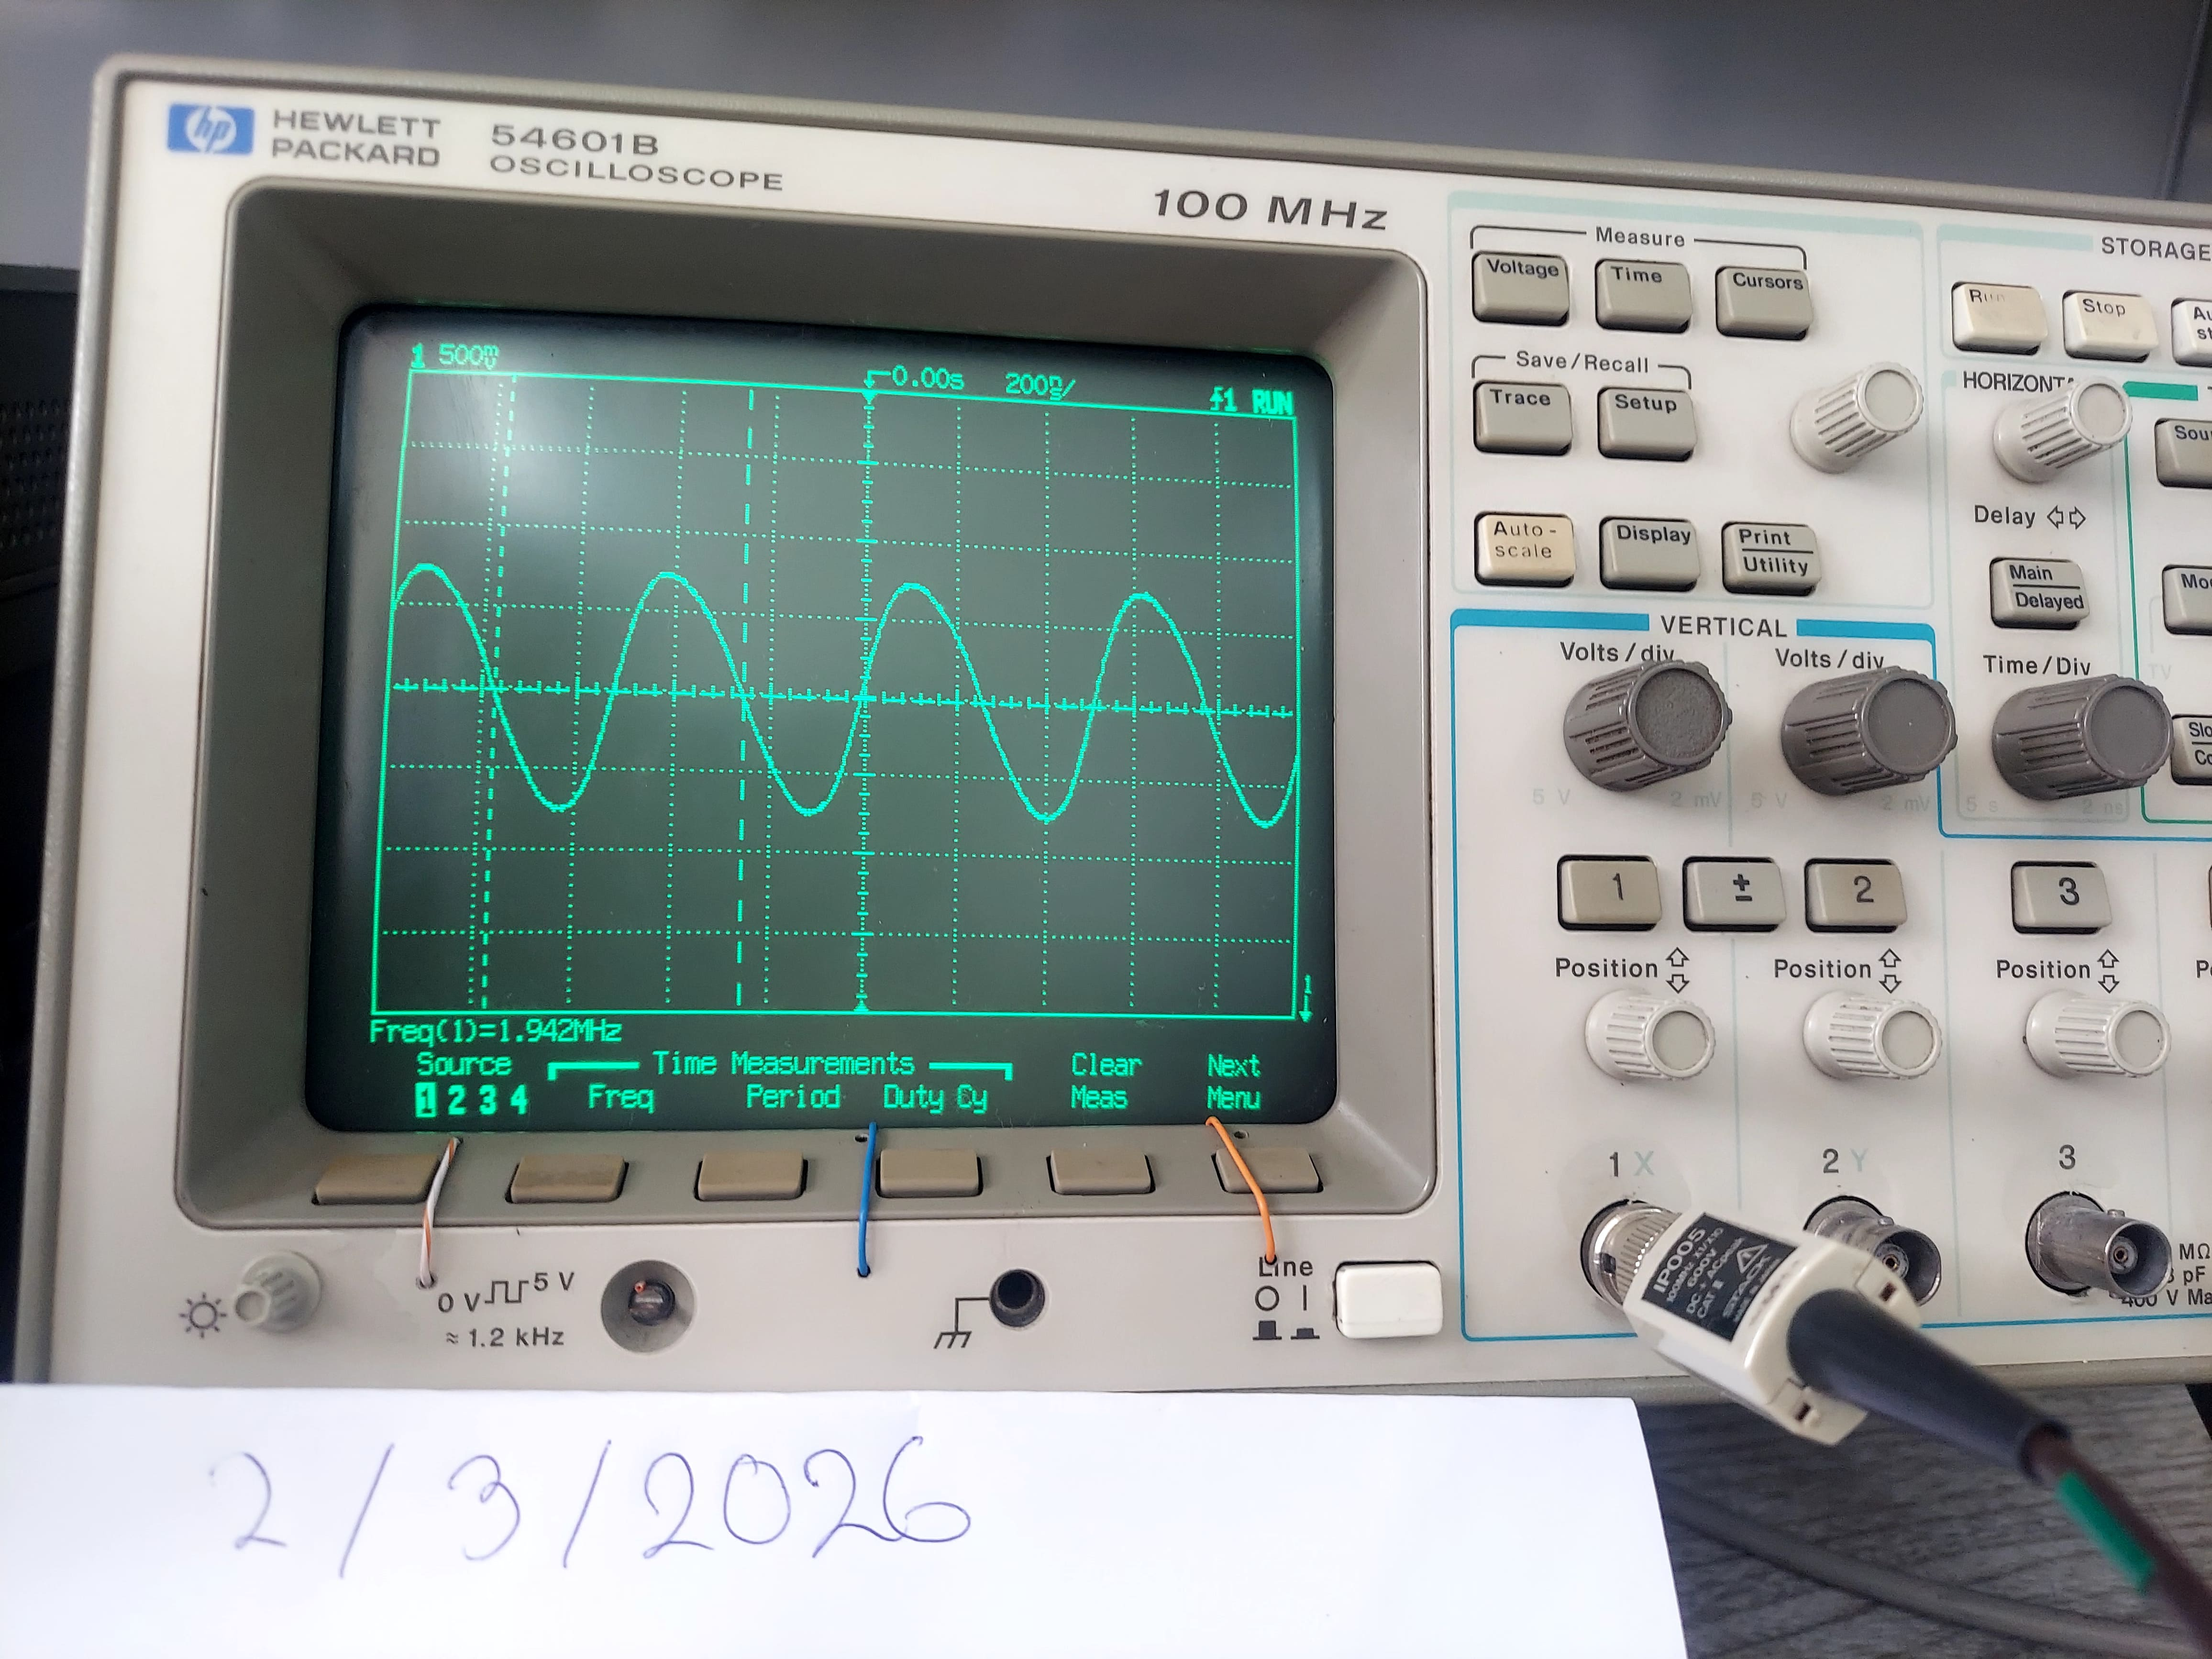
\includegraphics[width=0.8\textwidth]{Imagenes/3-reloj-universal-b.jpg}
%     \caption{Señal de reloj B}
% \end{figure}

% \begin{figure}[H]
%     \centering
%     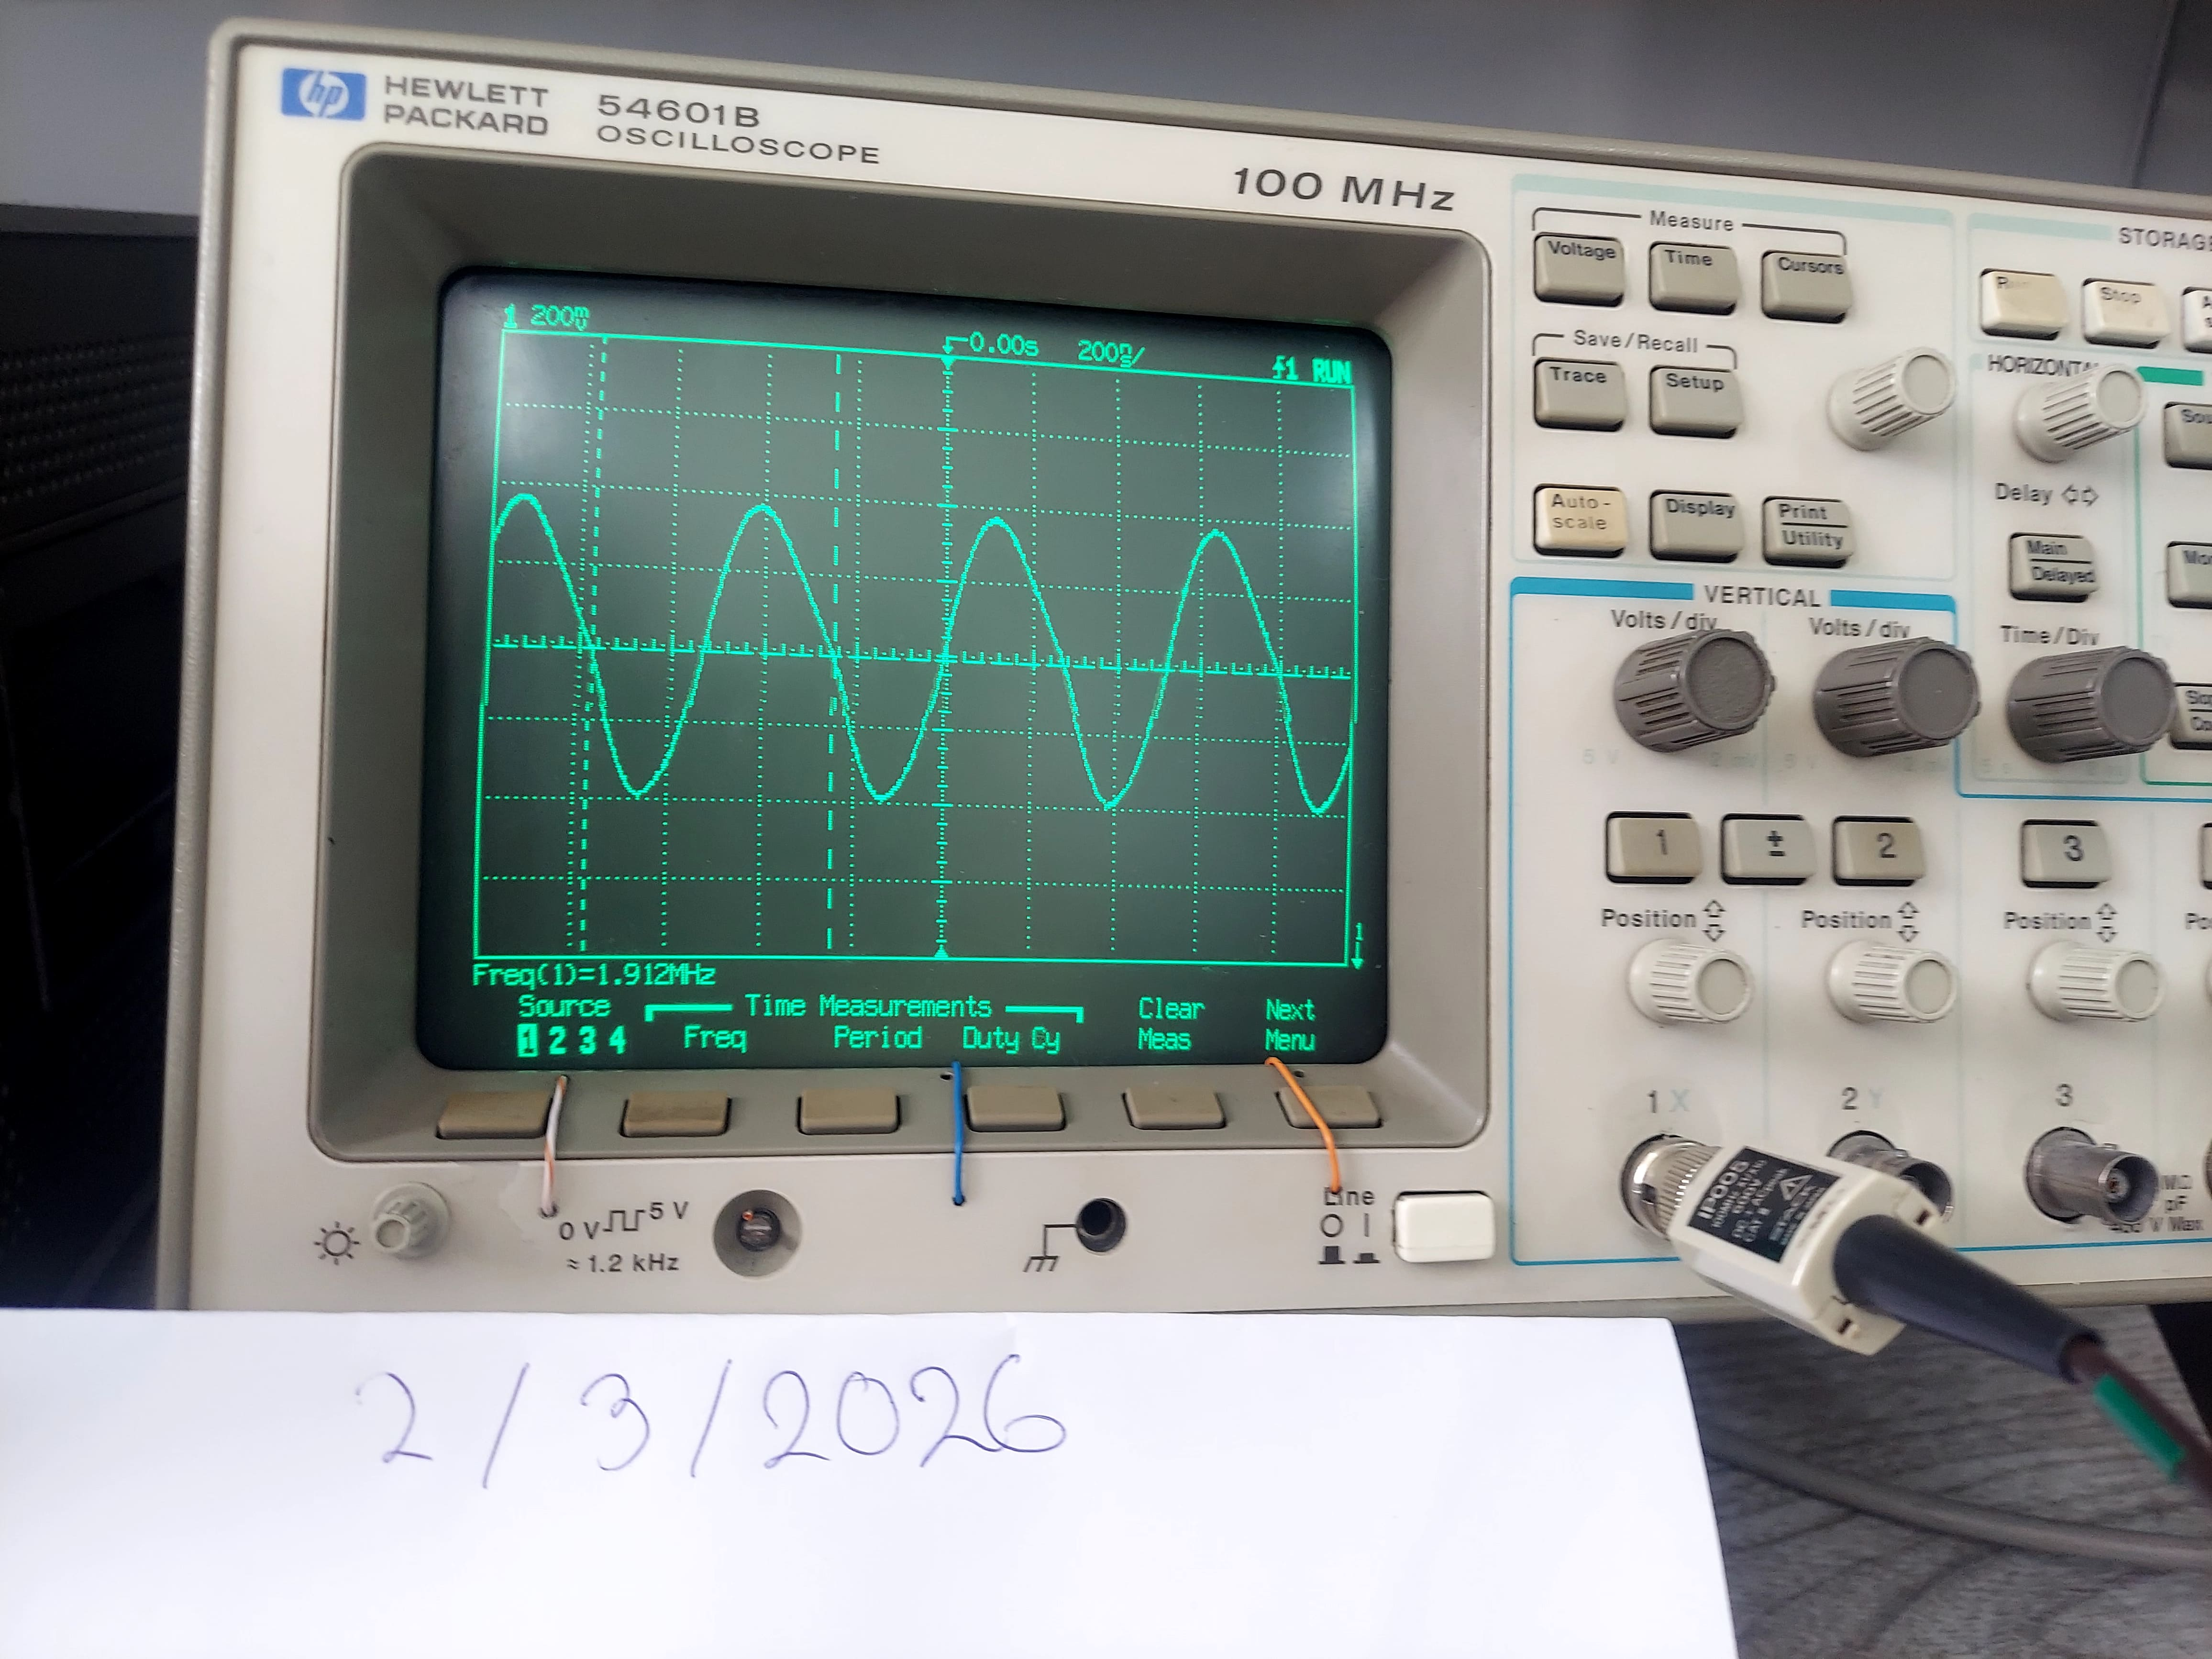
\includegraphics[width=0.8\textwidth]{Imagenes/3-reloj-universal-c.jpg}
%     \caption{Señal de reloj C}
% \end{figure}

% \begin{figure}[H]
%     \centering
%     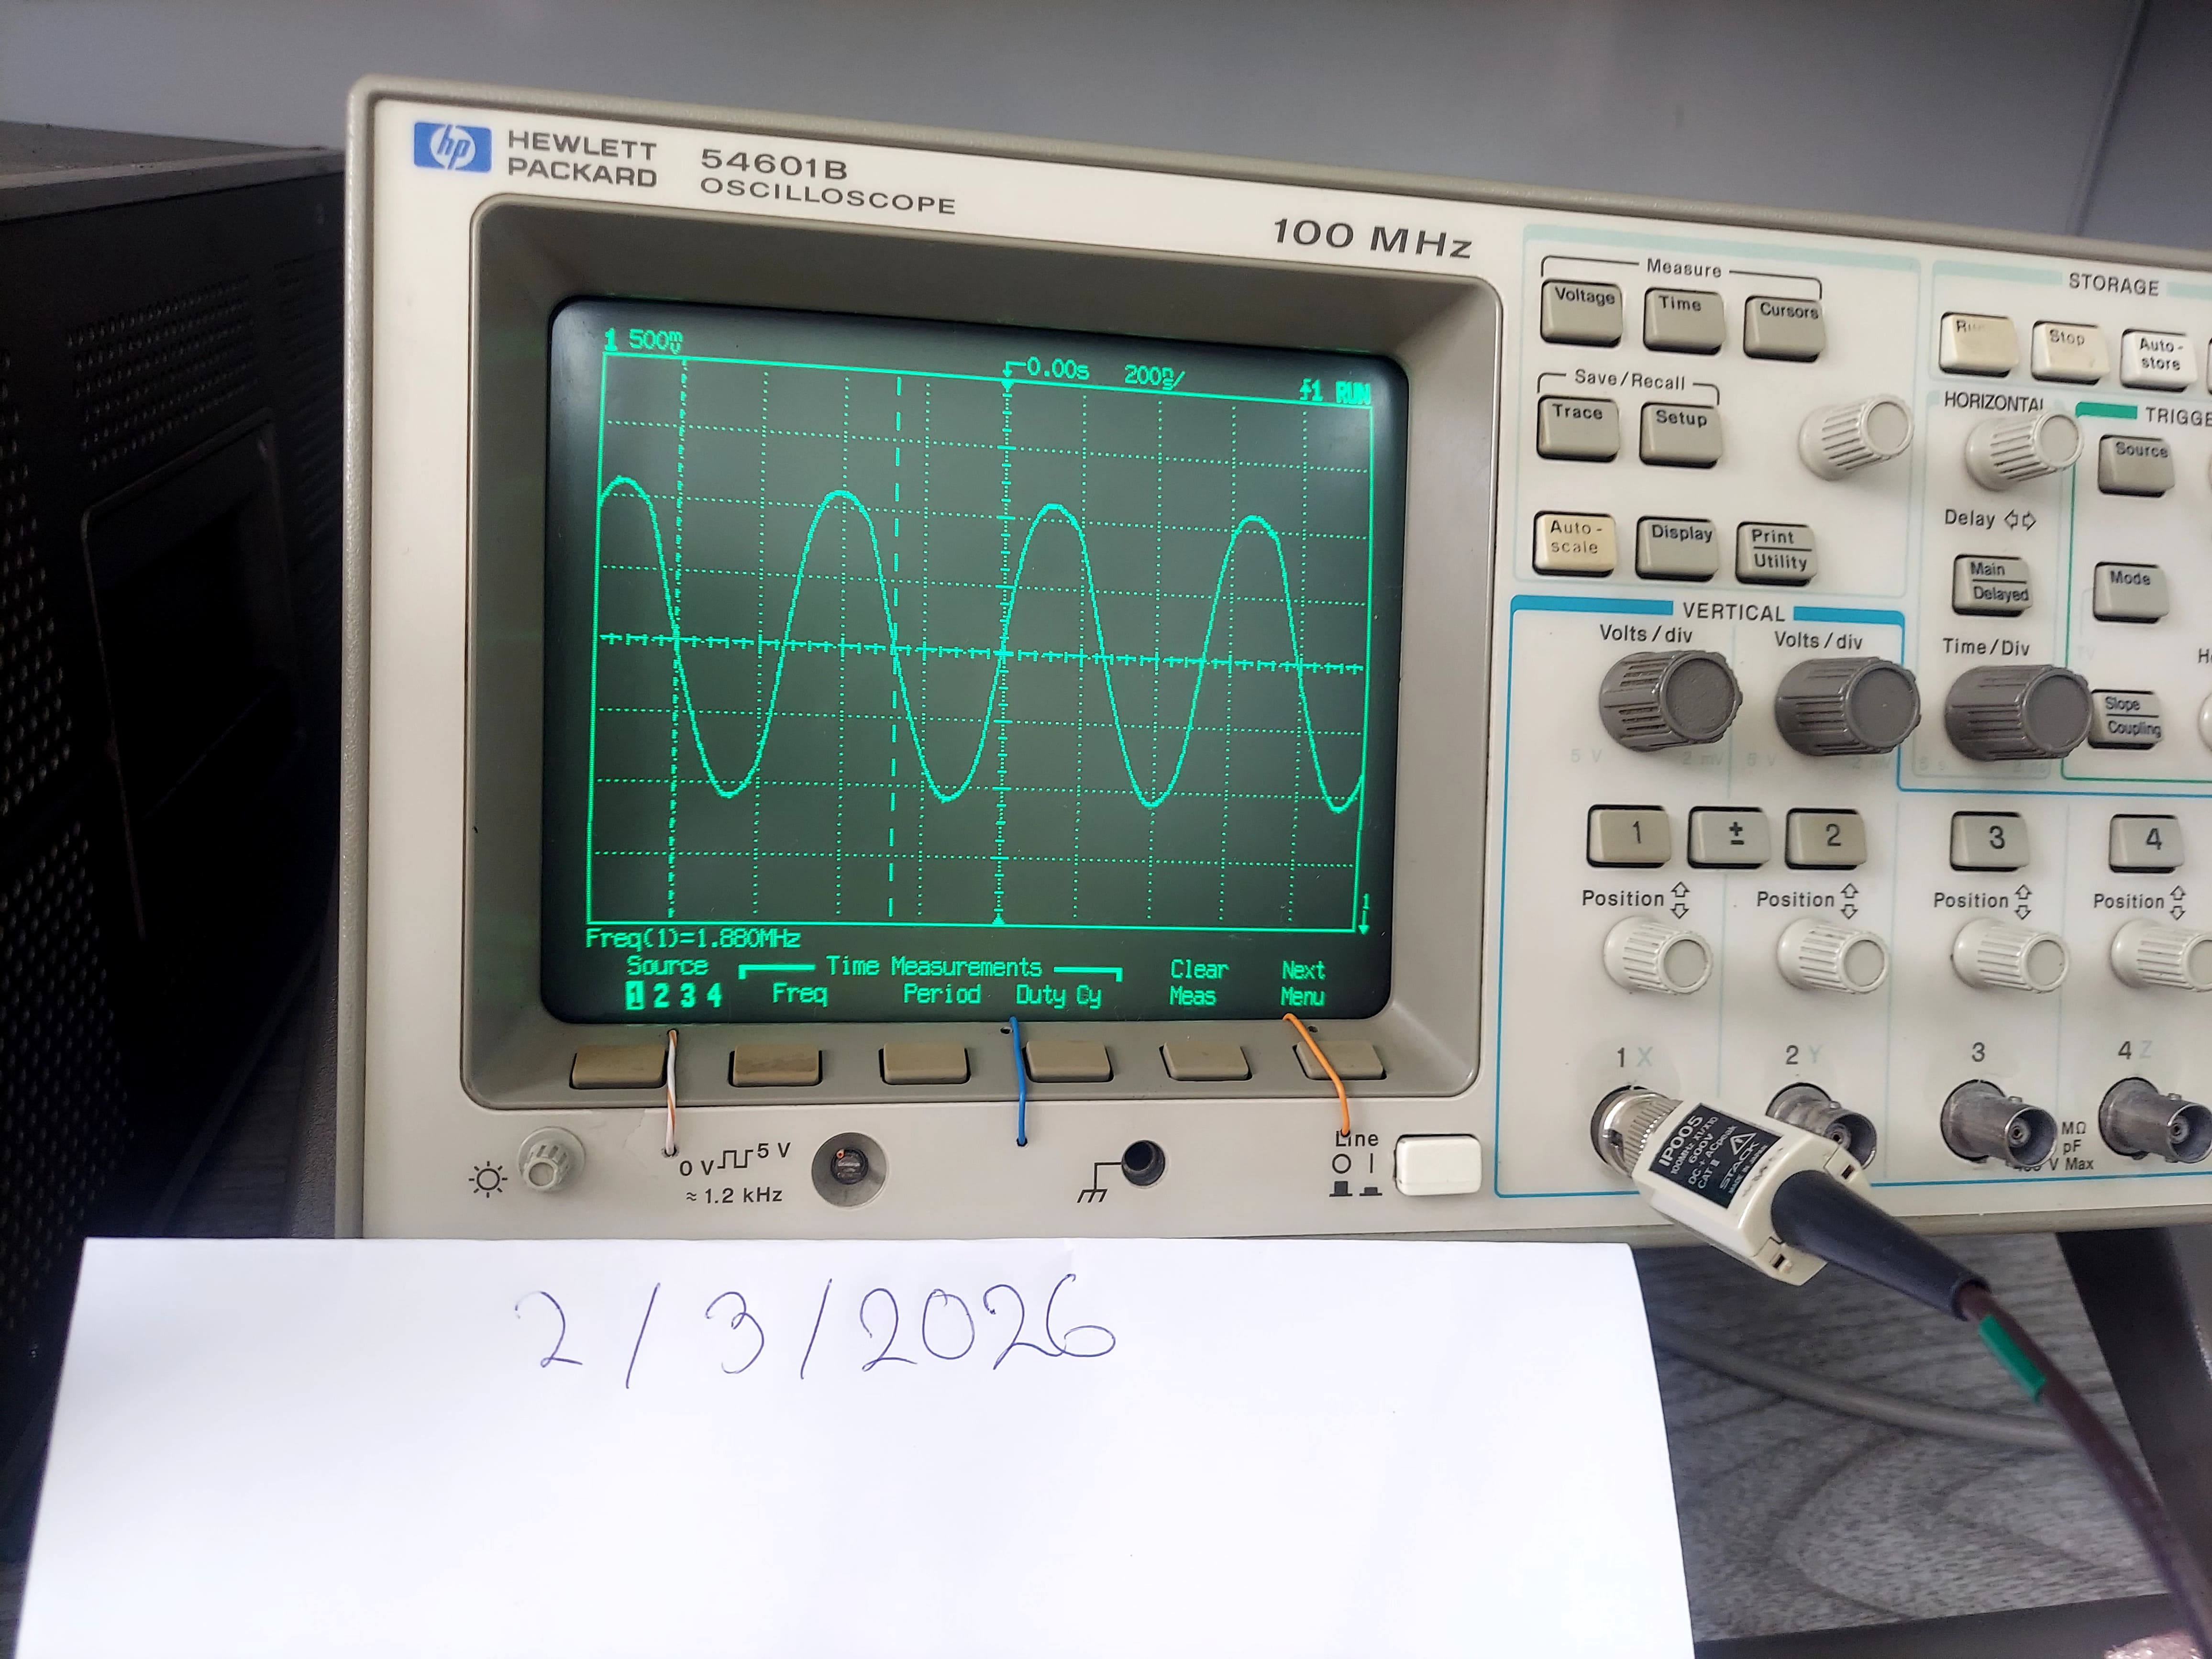
\includegraphics[width=0.8\textwidth]{Imagenes/3-reloj-universal-d.jpg}
%     \caption{Señal de reloj D}
% \end{figure}

\subsection{Paso 4: Muestreo y Retención}
\textbf{Instrucciones:}
\begin{itemize}
    \item Conecte en el punto señalado como Vin una señal senoidal de aproximadamente 1 KHz y accione el switch 8 de SWc.
    \item Seleccione el condensador C3 con el switch 2 de SWc.
    \item Coloque la señal de entrada, del punto TP5, en el canal A del osciloscopio y la señal muestreada (punto TP7) en el canal B. Observe el efecto de muestreo. ¿Cuántas muestras por período hay?
    \item Varíe la frecuencia de la senoidal a muestrear, llegando incluso a superar la frecuencia de Nyquist. Observe las señales de salida.
\end{itemize}

\begin{figure}[H]
    \centering
    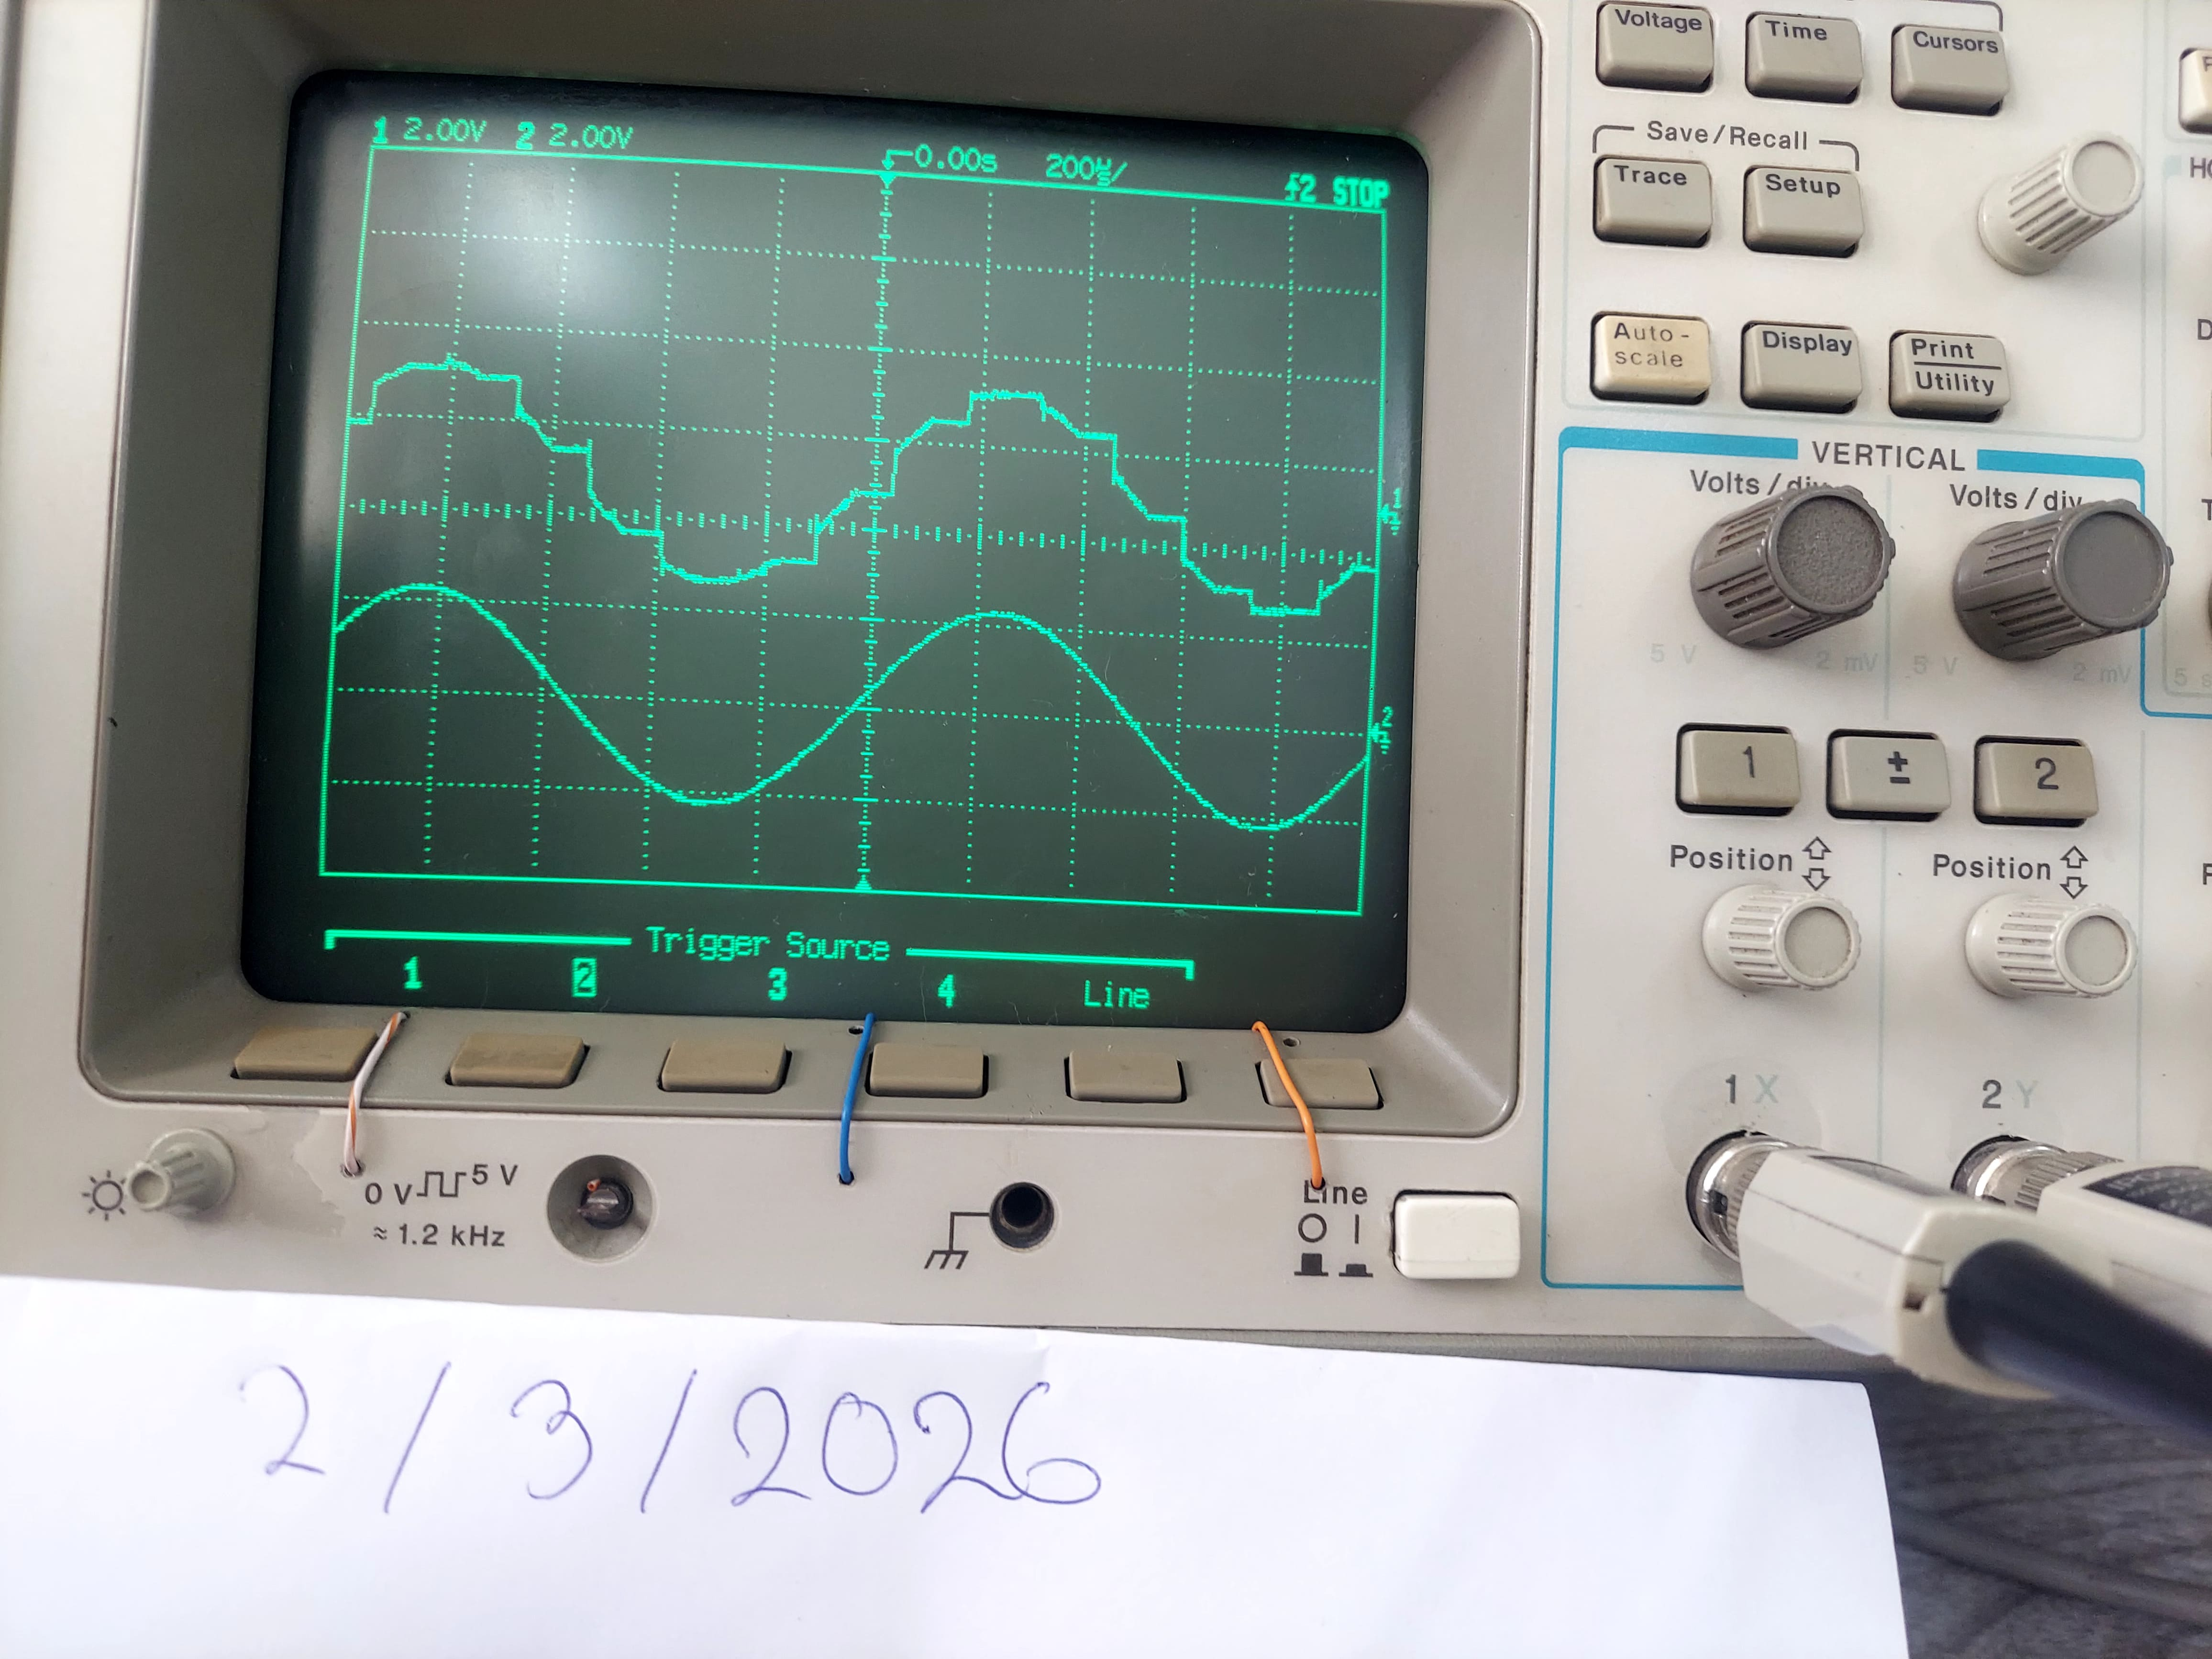
\includegraphics[width=0.8\textwidth]{Imagenes/4-muestreo-y-retencion-c.jpg}
    \caption{Configuración de muestreo y retención con C3.}
\end{figure}

\begin{figure}[H]
    \centering
    \begin{subfigure}[b]{0.45\textwidth}
        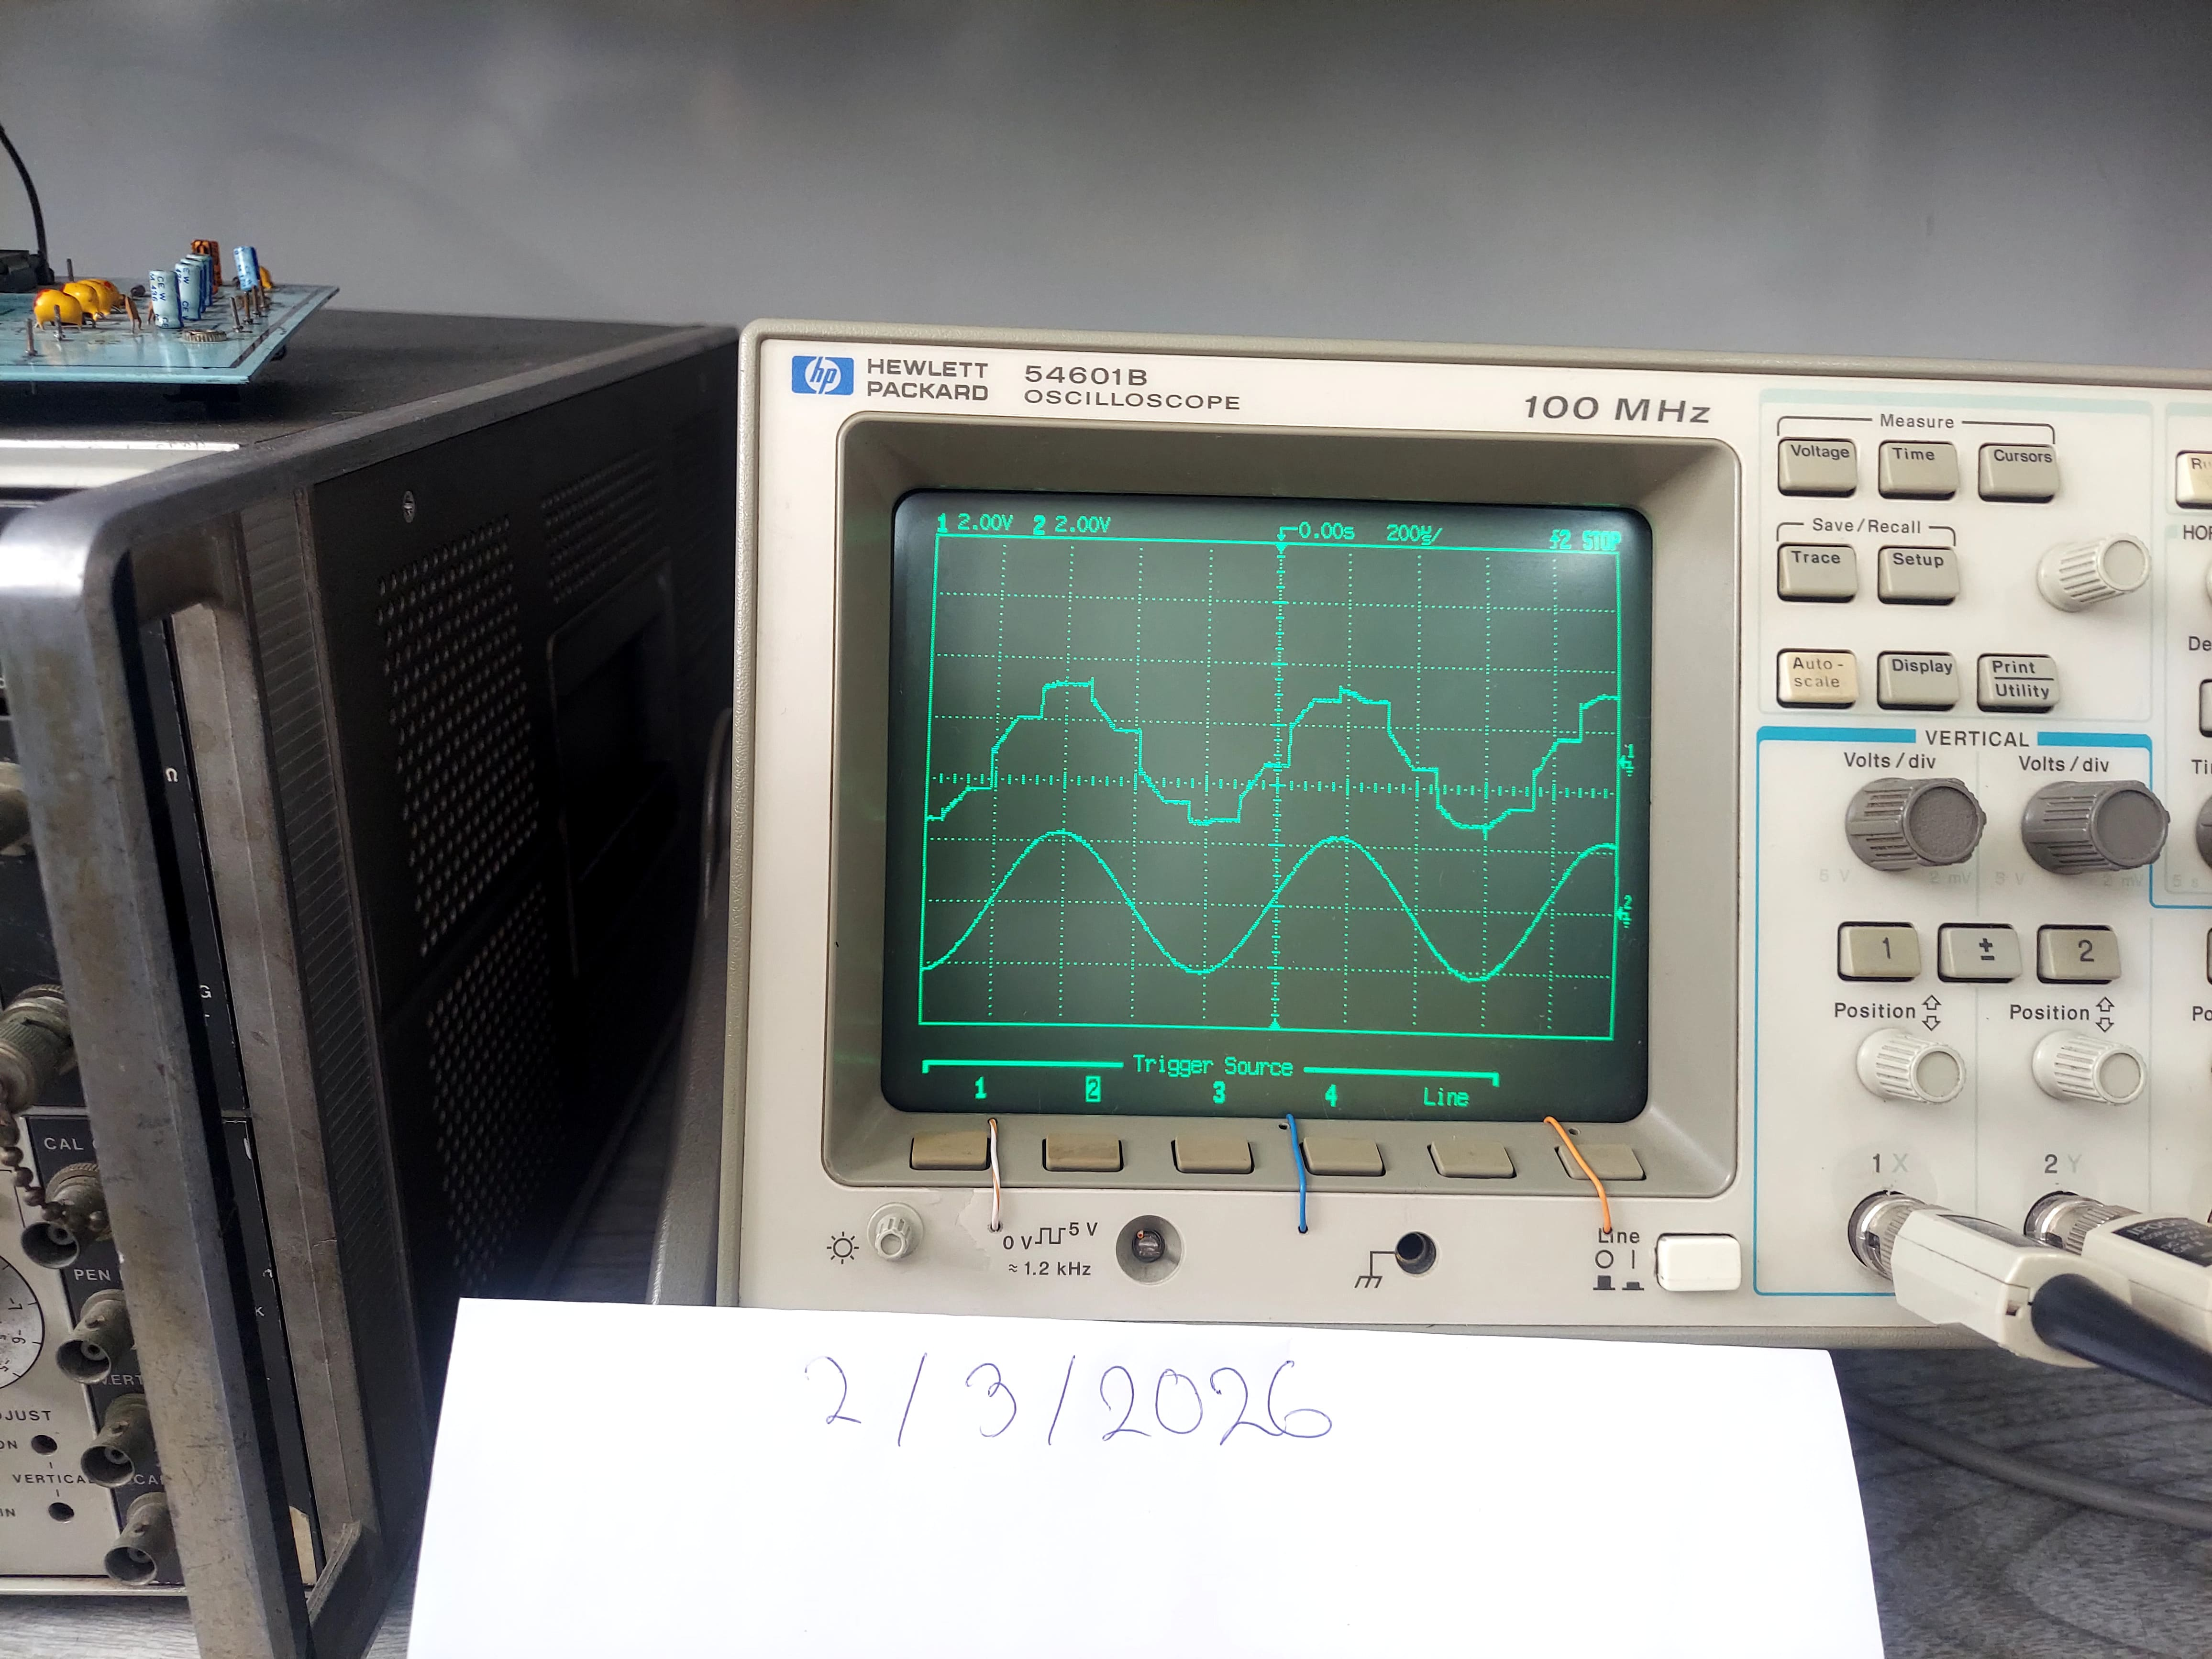
\includegraphics[width=\textwidth]{Imagenes/4-muestreo-y-retencion-d1.jpg}
        \caption{Muestra 1}
    \end{subfigure}
    \hfill
    \begin{subfigure}[b]{0.45\textwidth}
        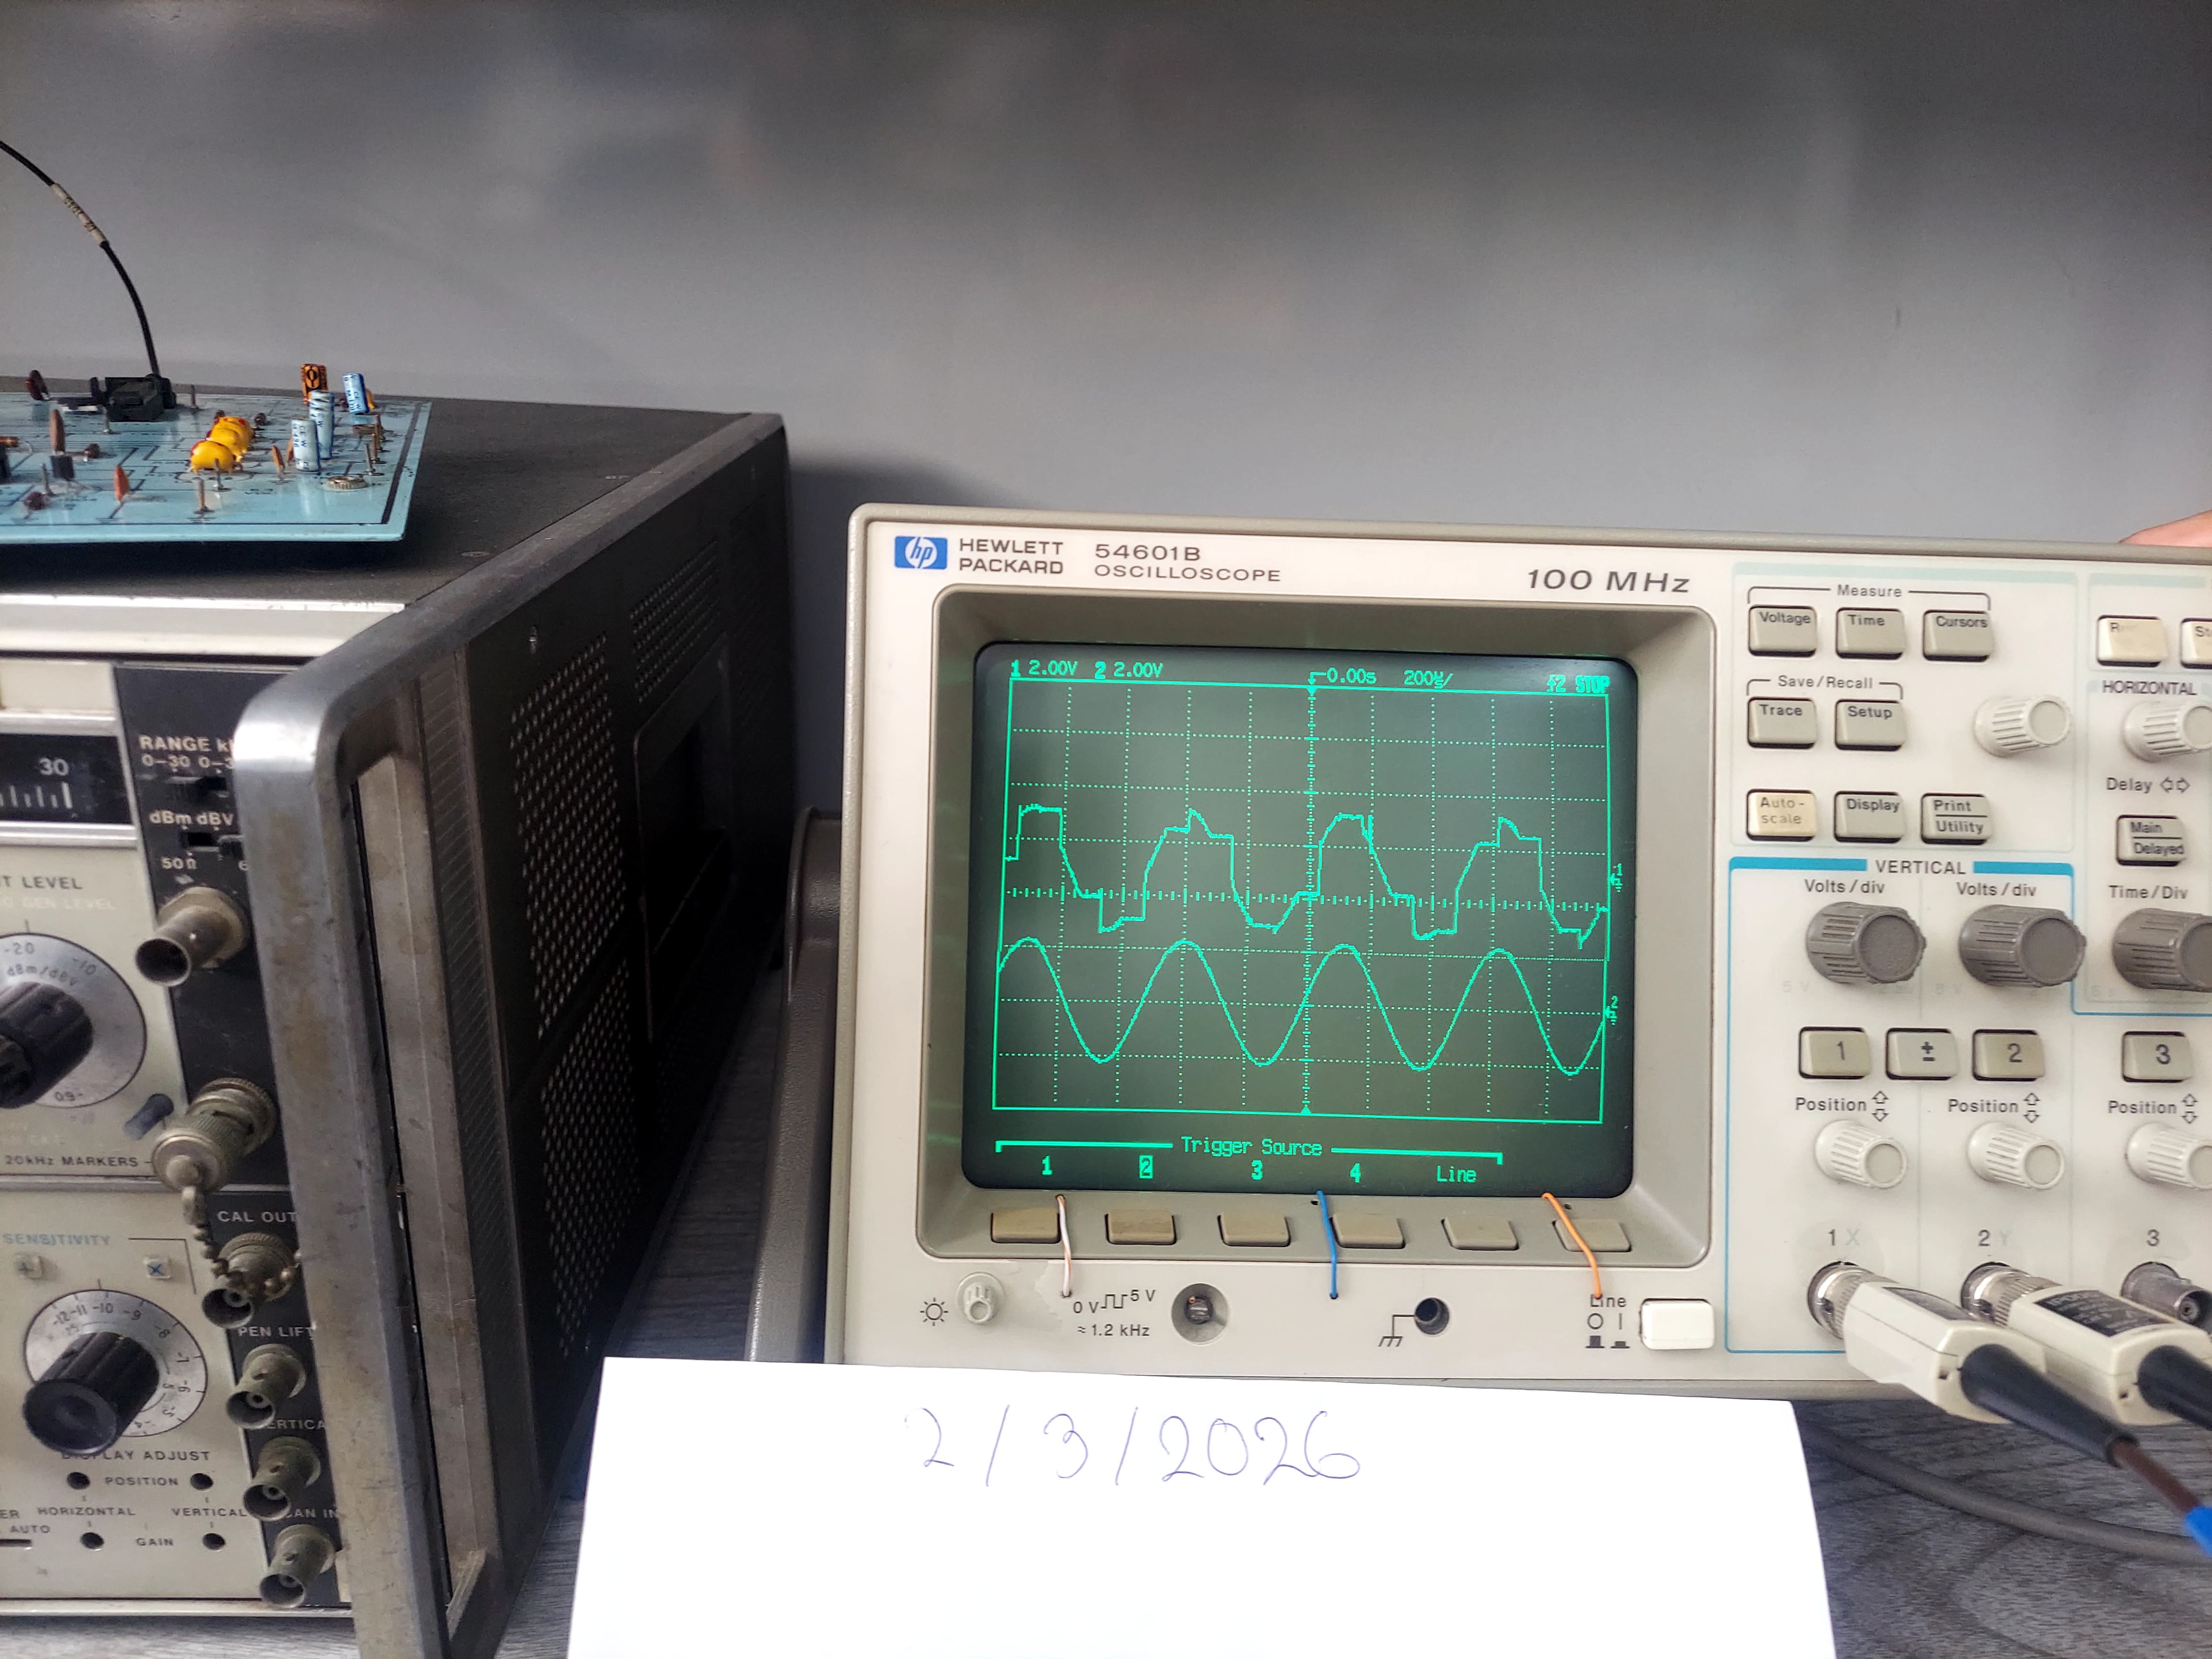
\includegraphics[width=\textwidth]{Imagenes/4-muestreo-y-retencion-d2.jpg}
        \caption{Muestra 2}
    \end{subfigure}
    \\[2ex]
    \begin{subfigure}[b]{0.45\textwidth}
        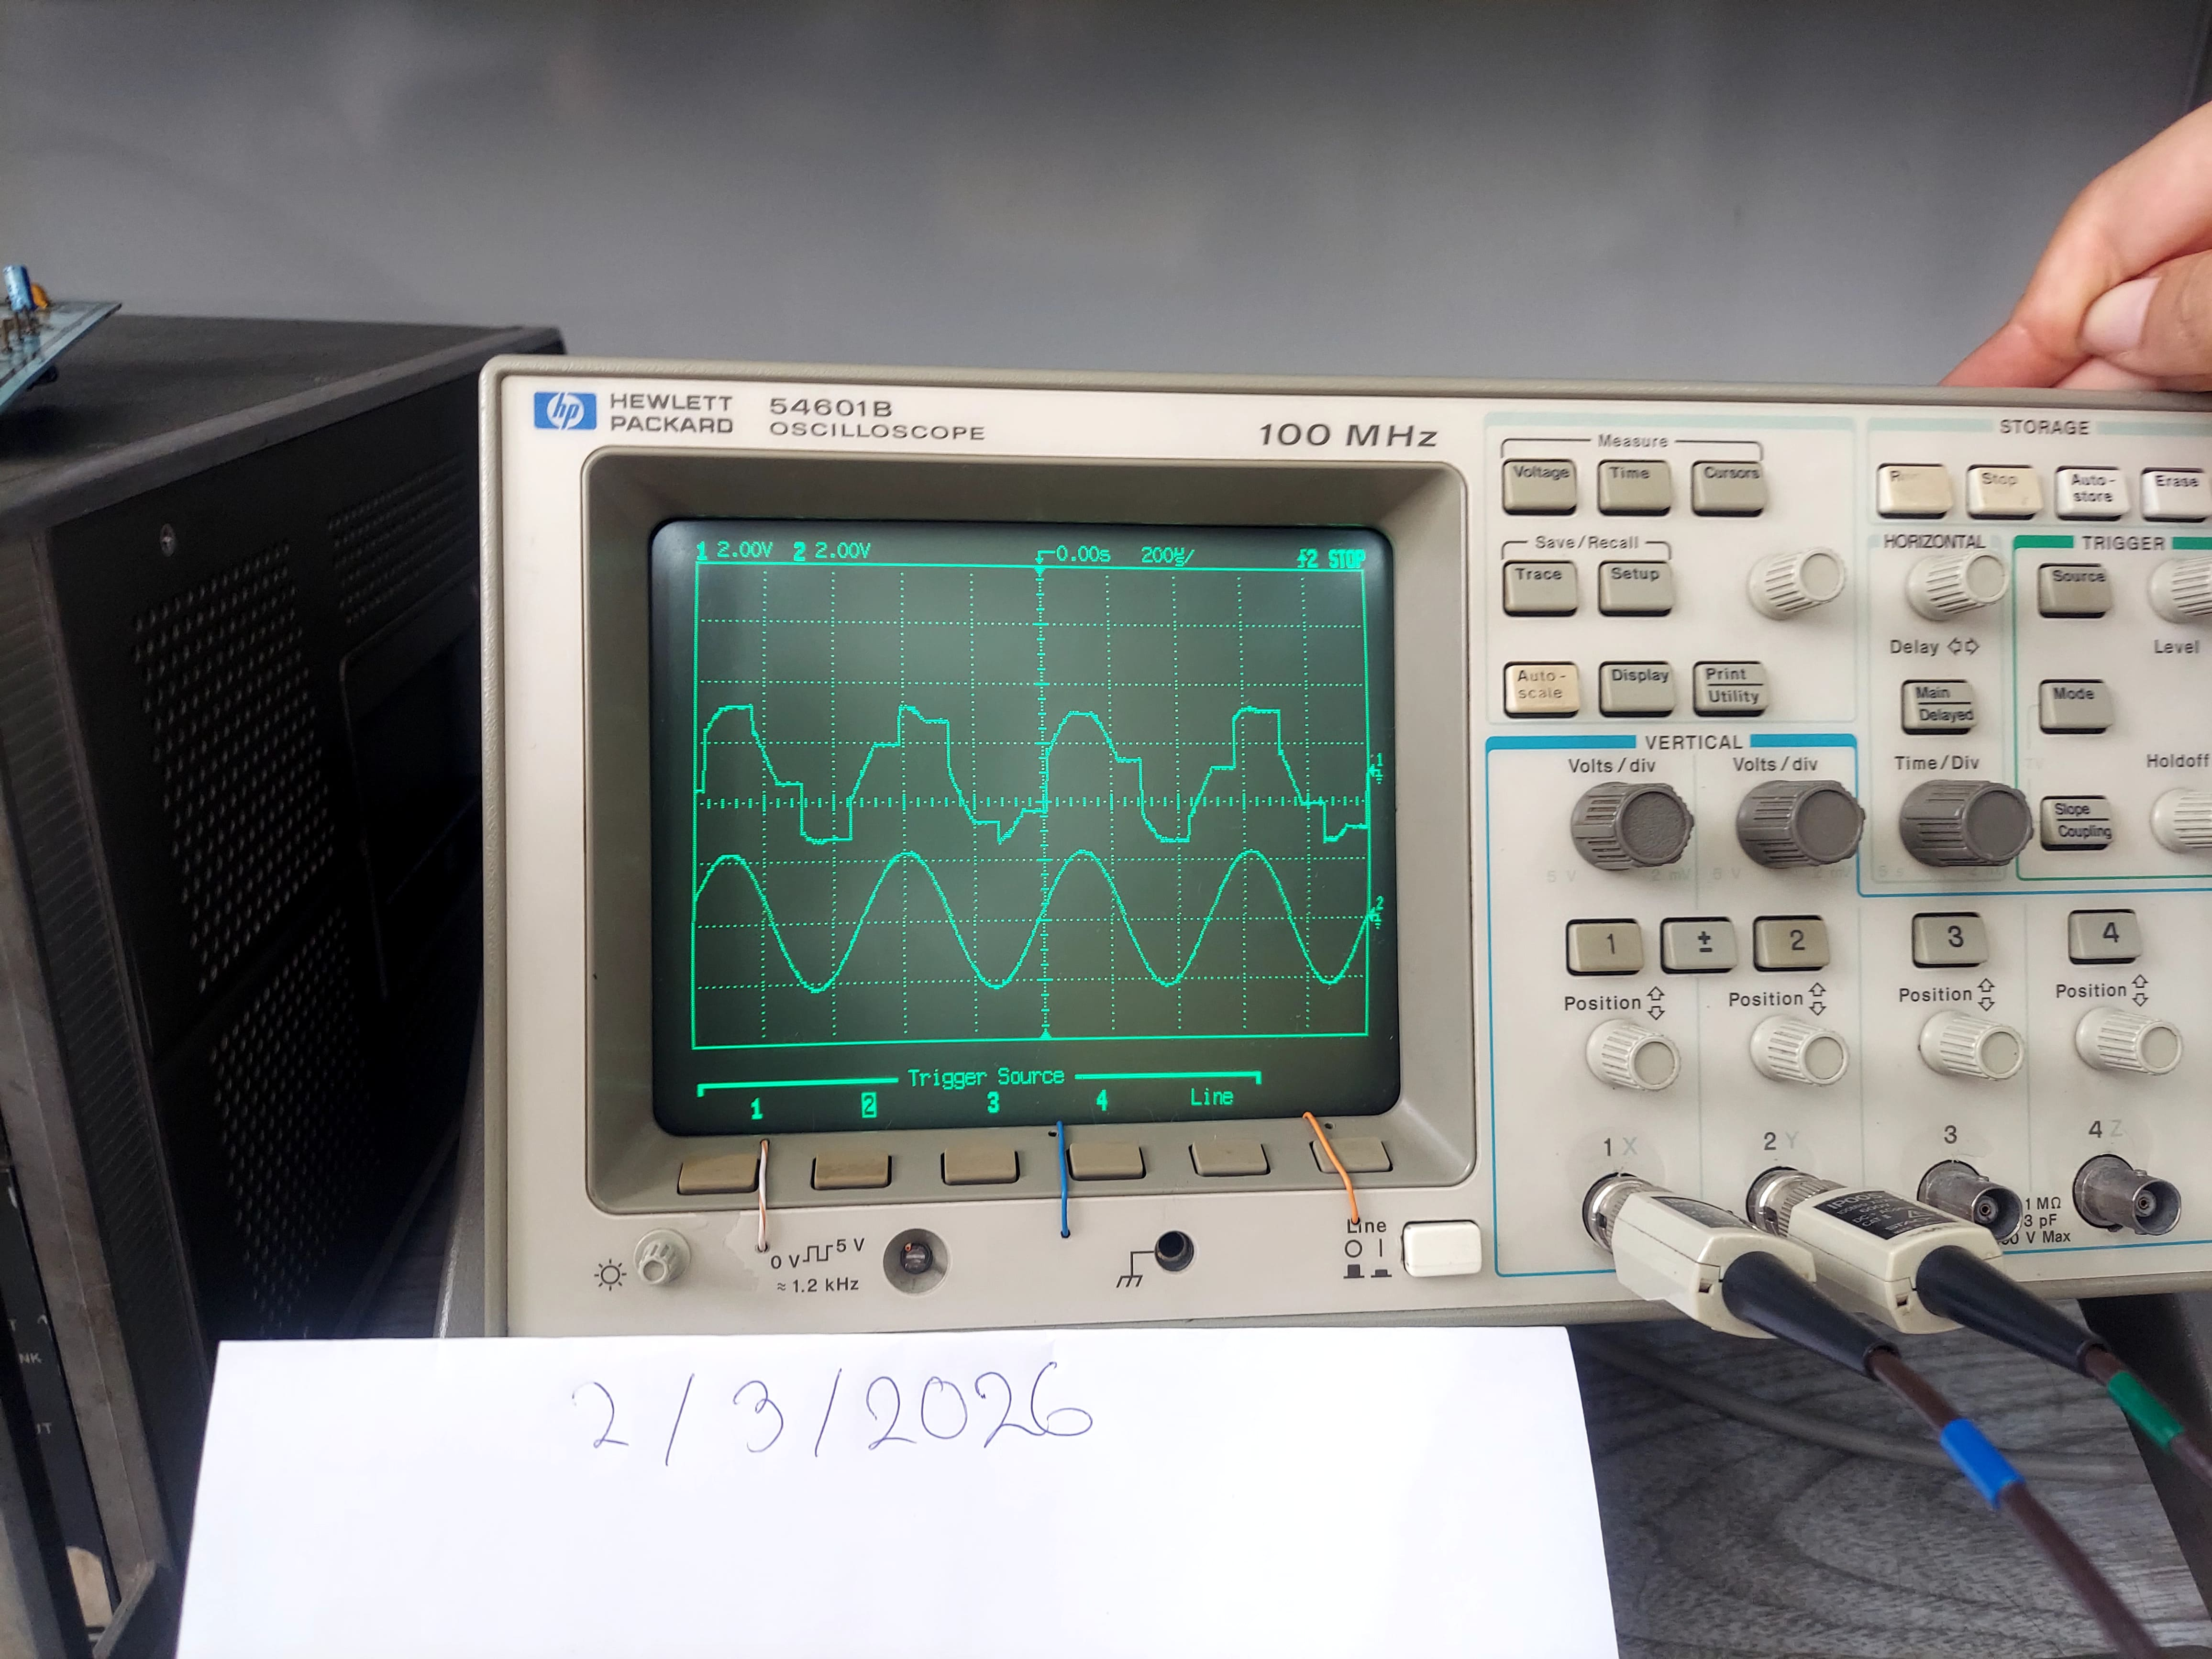
\includegraphics[width=\textwidth]{Imagenes/4-muestreo-y-retencion-d3.jpg}
        \caption{Muestra 3}
    \end{subfigure}
    \hfill
    \begin{subfigure}[b]{0.45\textwidth}
        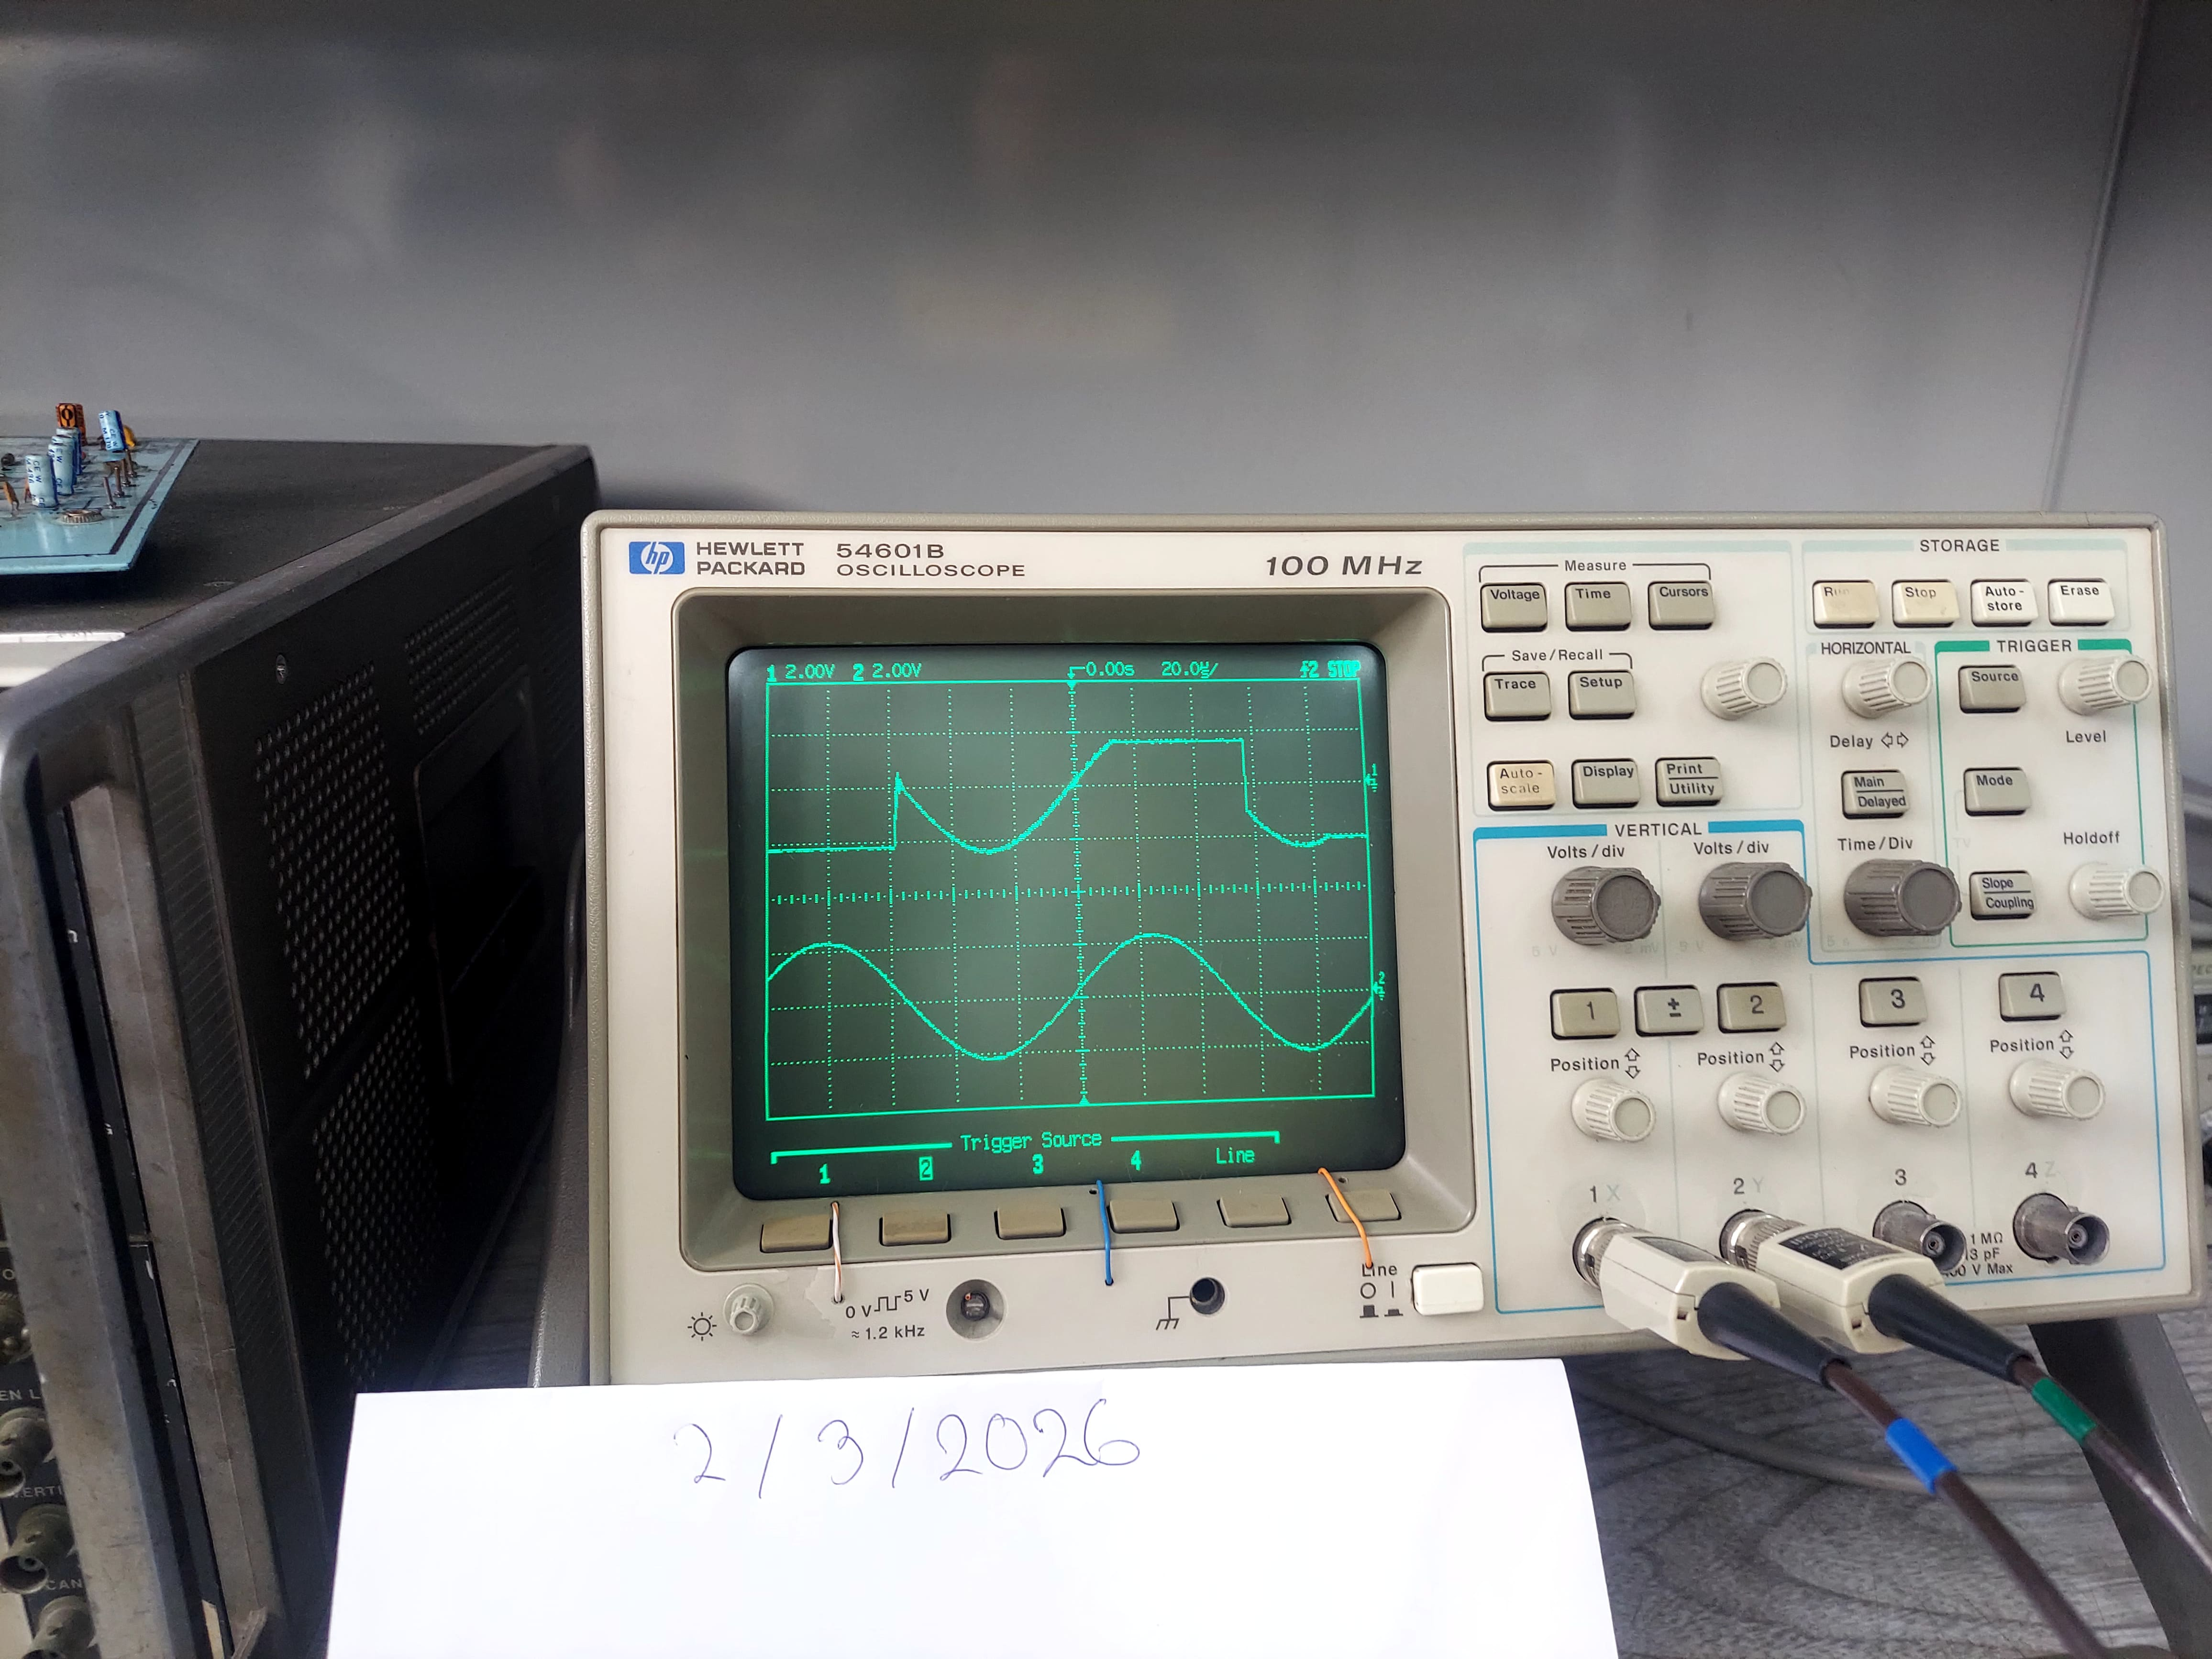
\includegraphics[width=\textwidth]{Imagenes/4-muestreo-y-retencion-d4.jpg}
        \caption{Muestra 4}
    \end{subfigure}
    \\[2ex]
    \begin{subfigure}[b]{0.45\textwidth}
        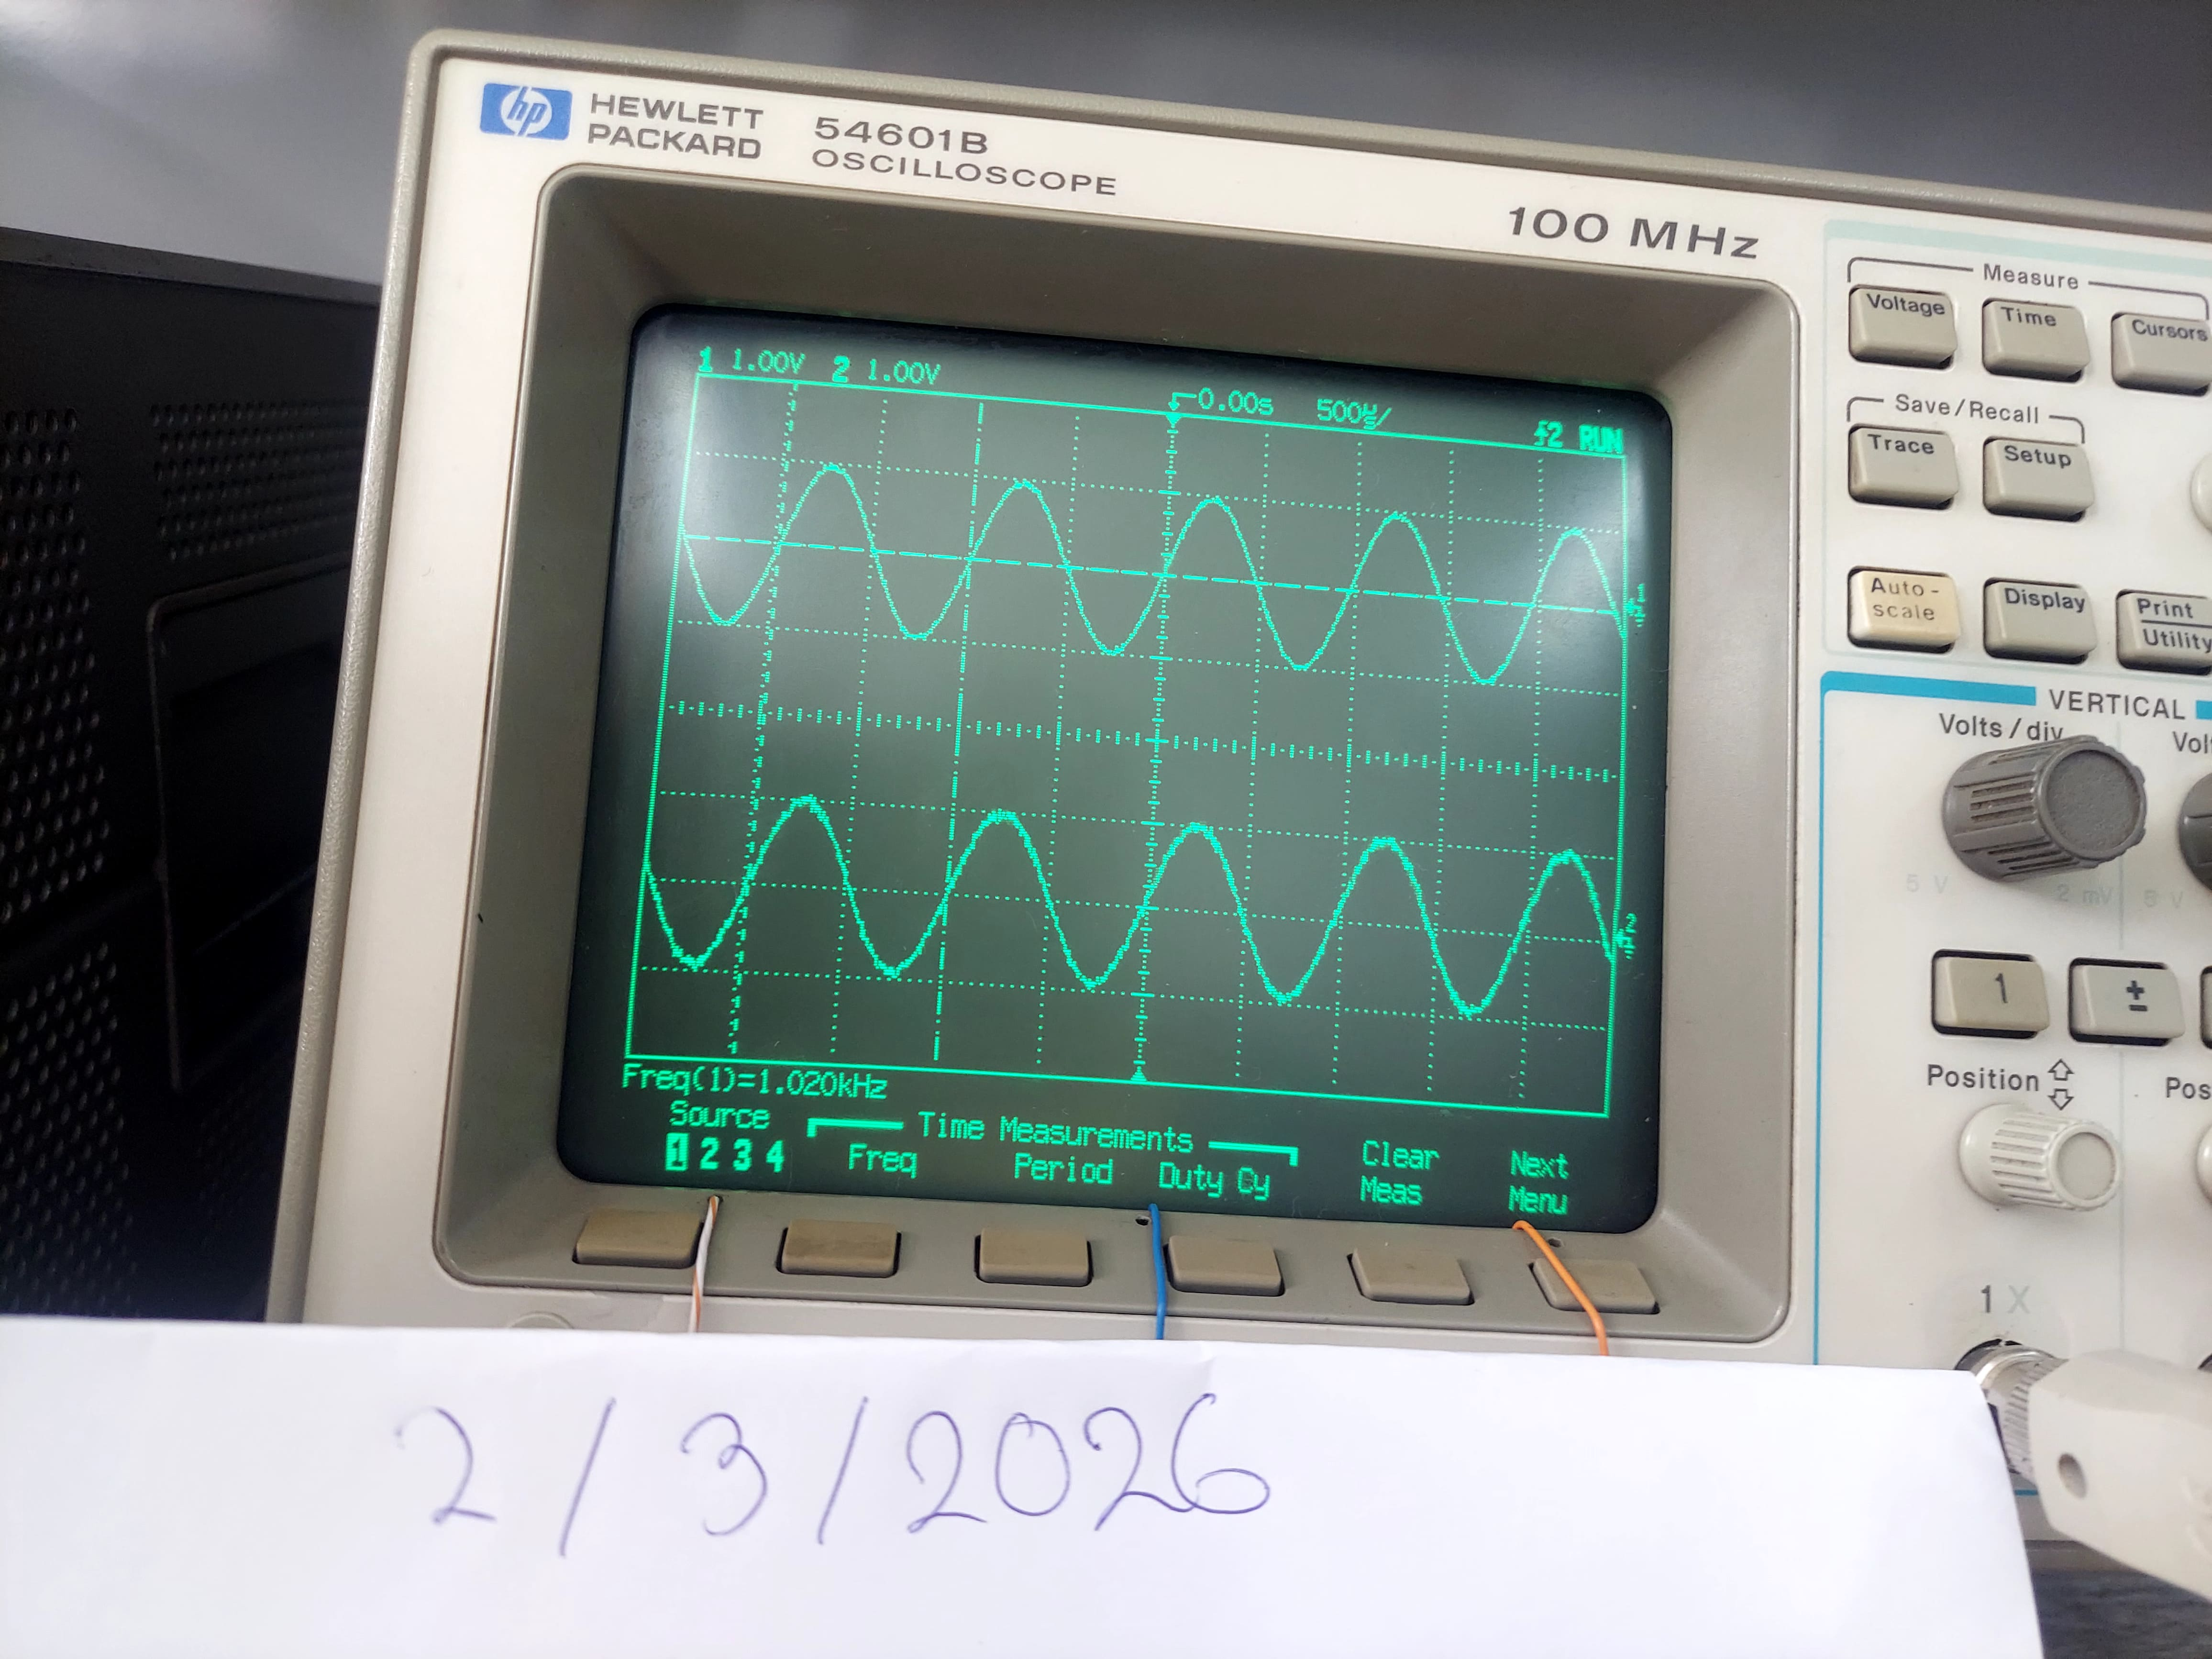
\includegraphics[width=\textwidth]{Imagenes/4-muestreo-y-retencion-d6.jpg}
        \caption{Muestra 5}
    \end{subfigure}
    \hfill
    \begin{subfigure}[b]{0.45\textwidth}
        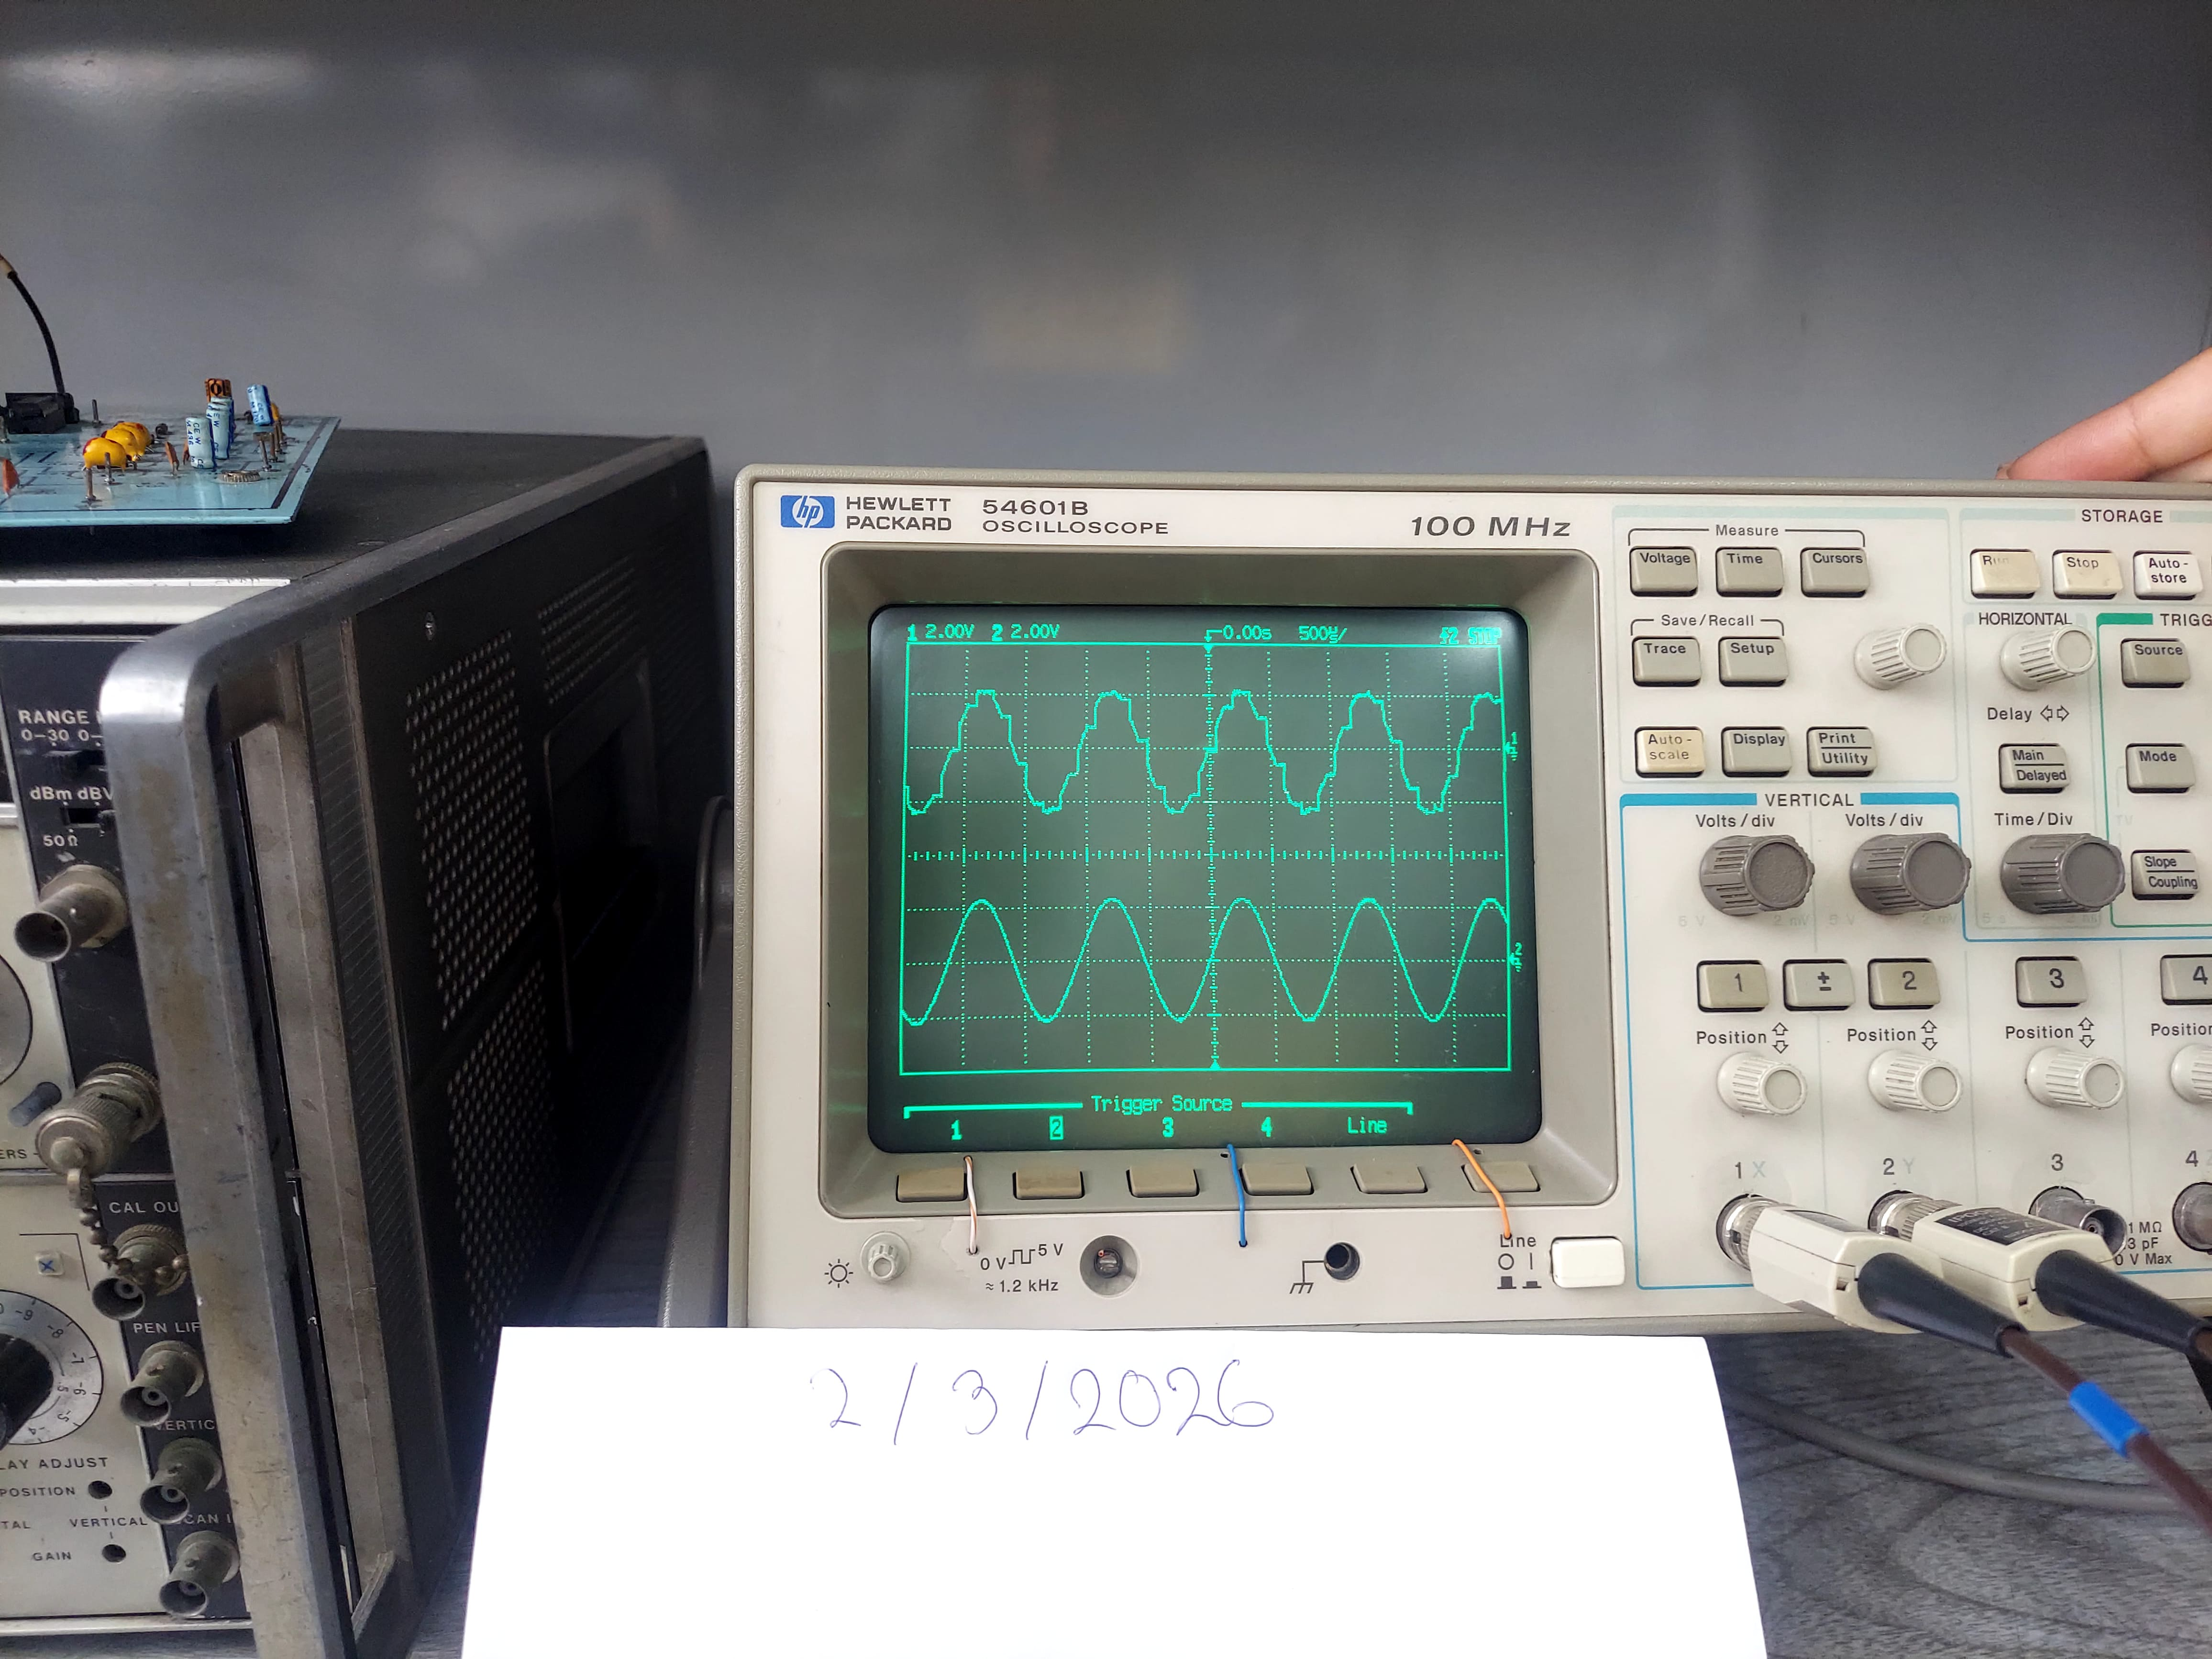
\includegraphics[width=\textwidth]{Imagenes/4-muestreo-y-retencion-d7.jpg}
        \caption{Muestra 6}
    \end{subfigure}
    \caption{Observación del efecto de muestreo al variar la frecuencia de entrada.}
\end{figure}

\subsection{Paso 5: Frecuencia de Reloj}
\textbf{Instrucciones:} Desconecte los puentes 1, 2, 3 y 4. Mida la frecuencia del reloj en TP8. Mida la frecuencia de muestreo en TP9 (señal multicanal a transmitir). Verifique la relación entre estas frecuencias.

\begin{figure}[H]
    \centering
    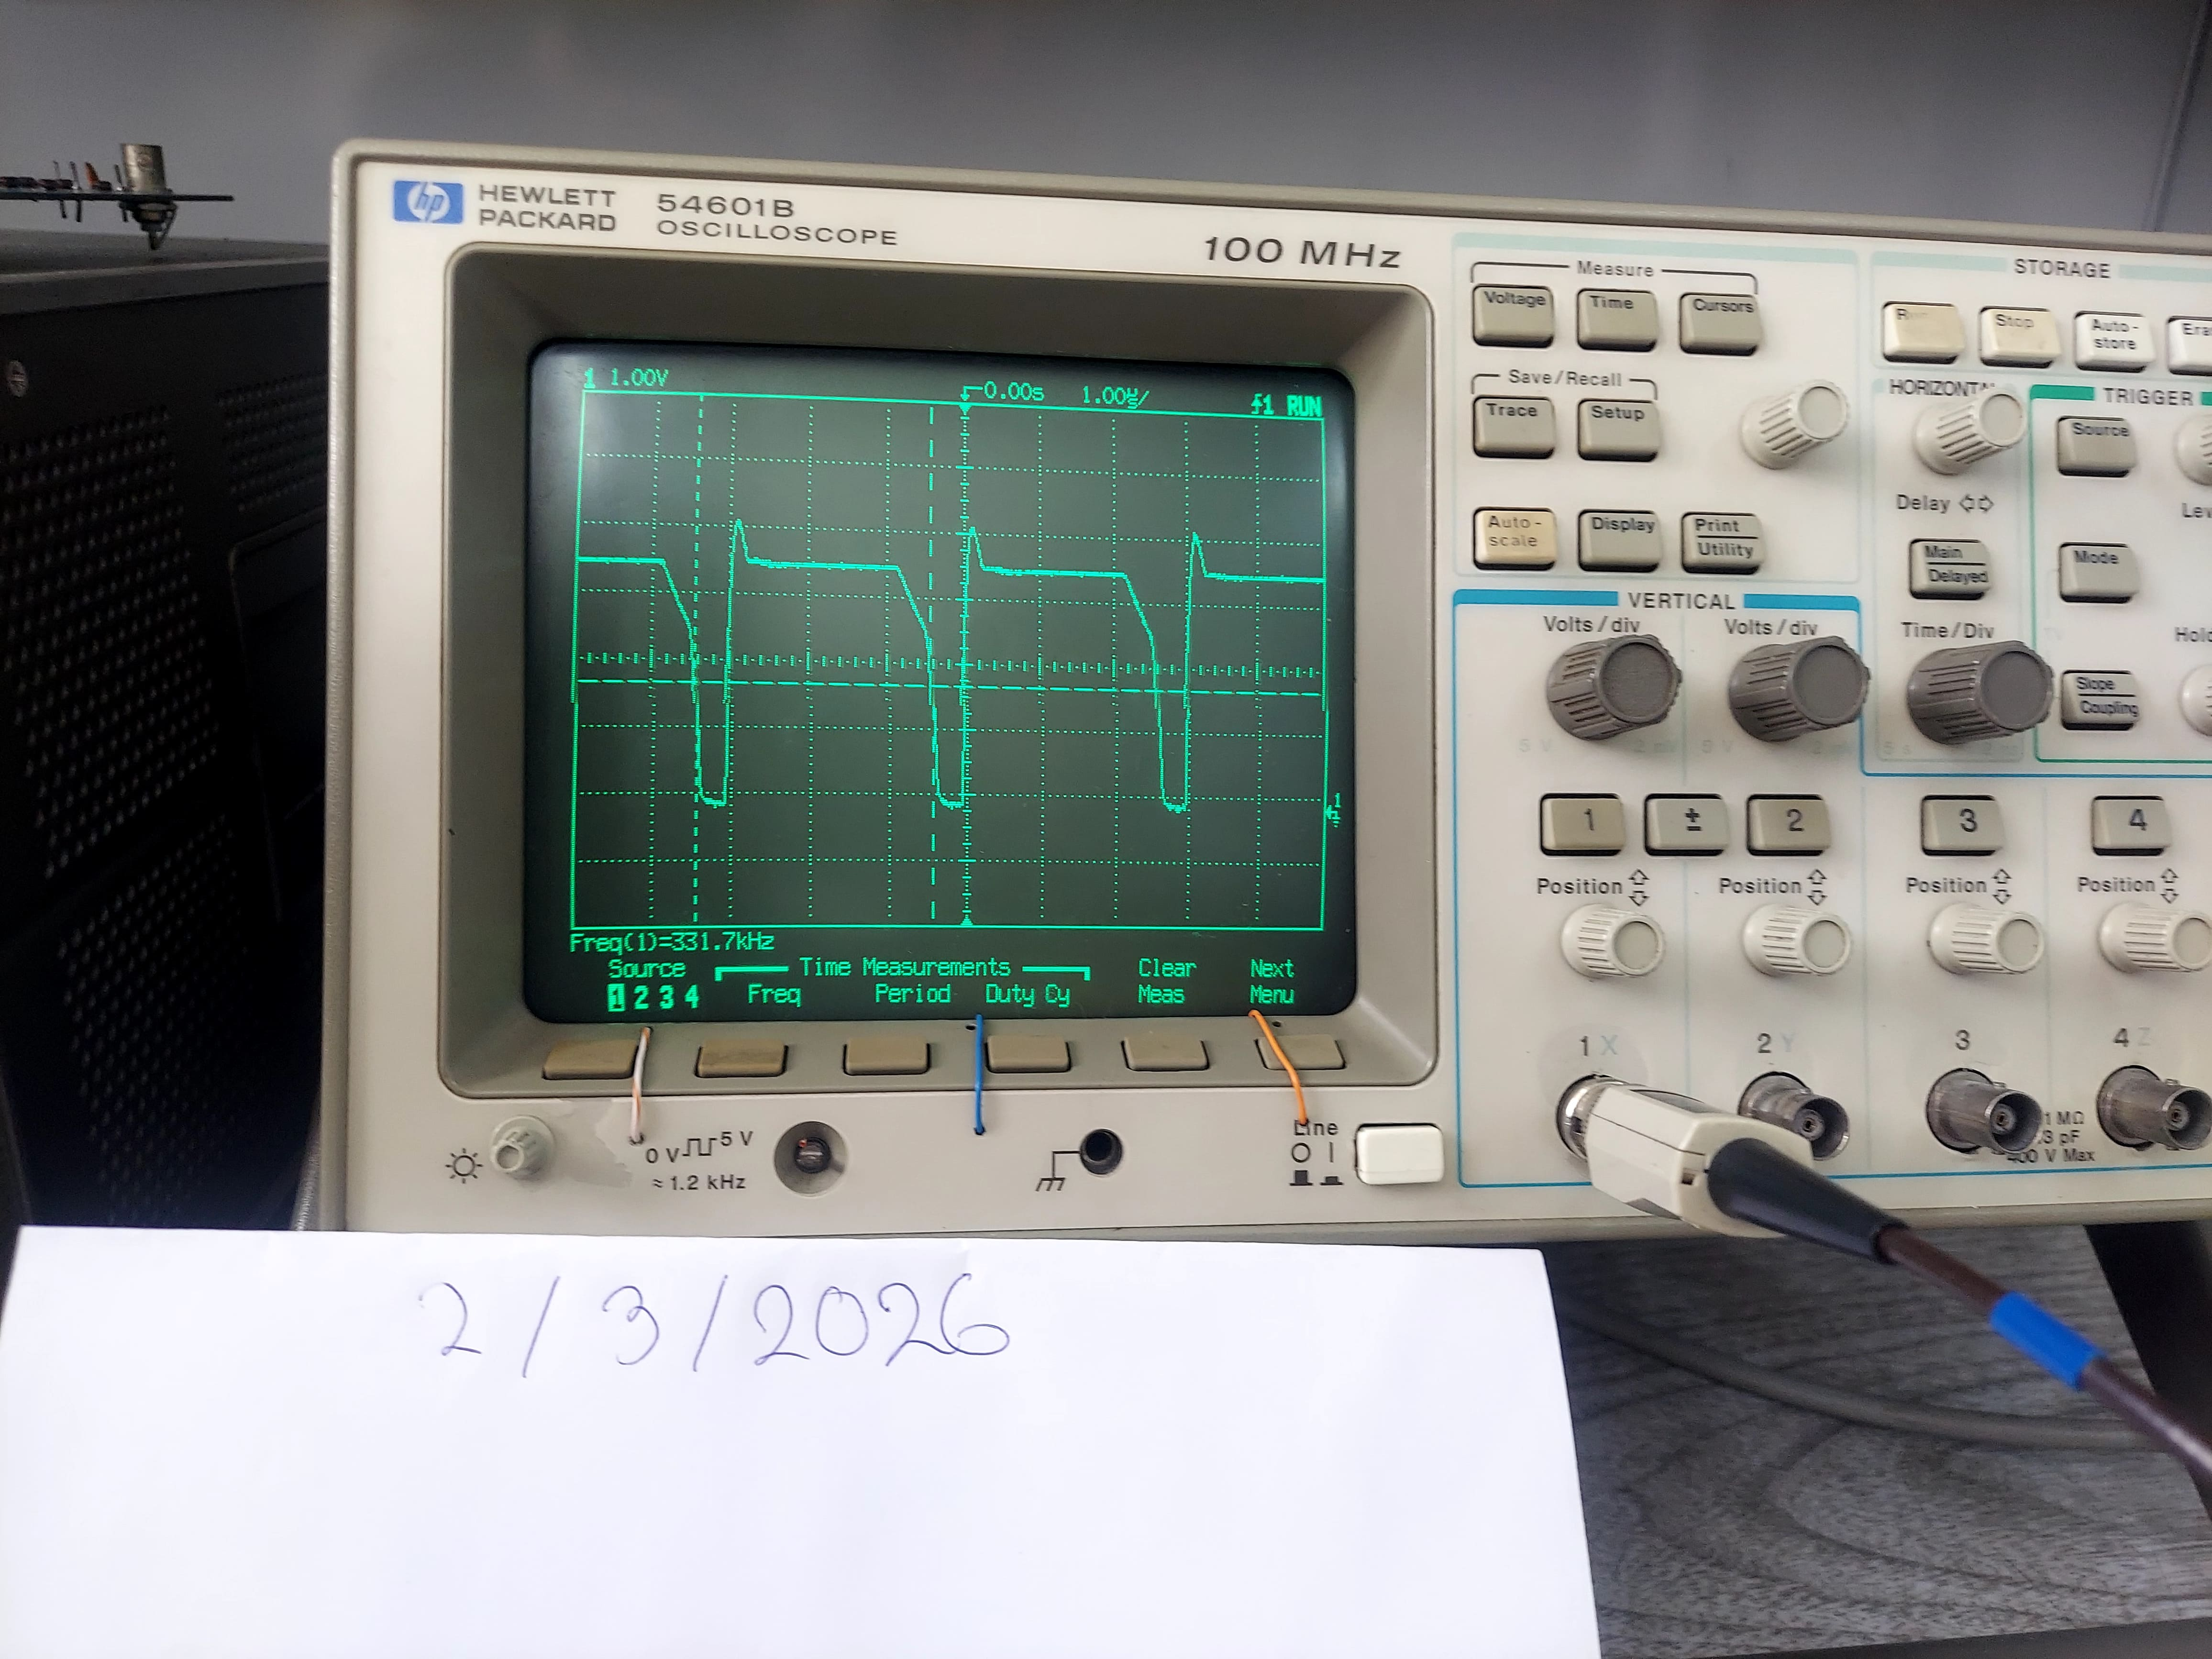
\includegraphics[width=0.8\textwidth]{Imagenes/5-frecuencia-de-reloj.jpg}
    \caption{Medición de frecuencia de reloj en TP8 y TP9.}
\end{figure}

\subsection{Paso 6: Señal Multicanal}
\textbf{Instrucciones:} Conectando progresivamente las señales por medio de los puentes 1, 2, 3 y 4 identifique la señal de sincronismo y los diferentes canales en el punto TP9. Dibuje y dimensiones la trama de la señal multicanal.

\begin{figure}[H]
    \centering
    \begin{subfigure}[b]{0.45\textwidth}
        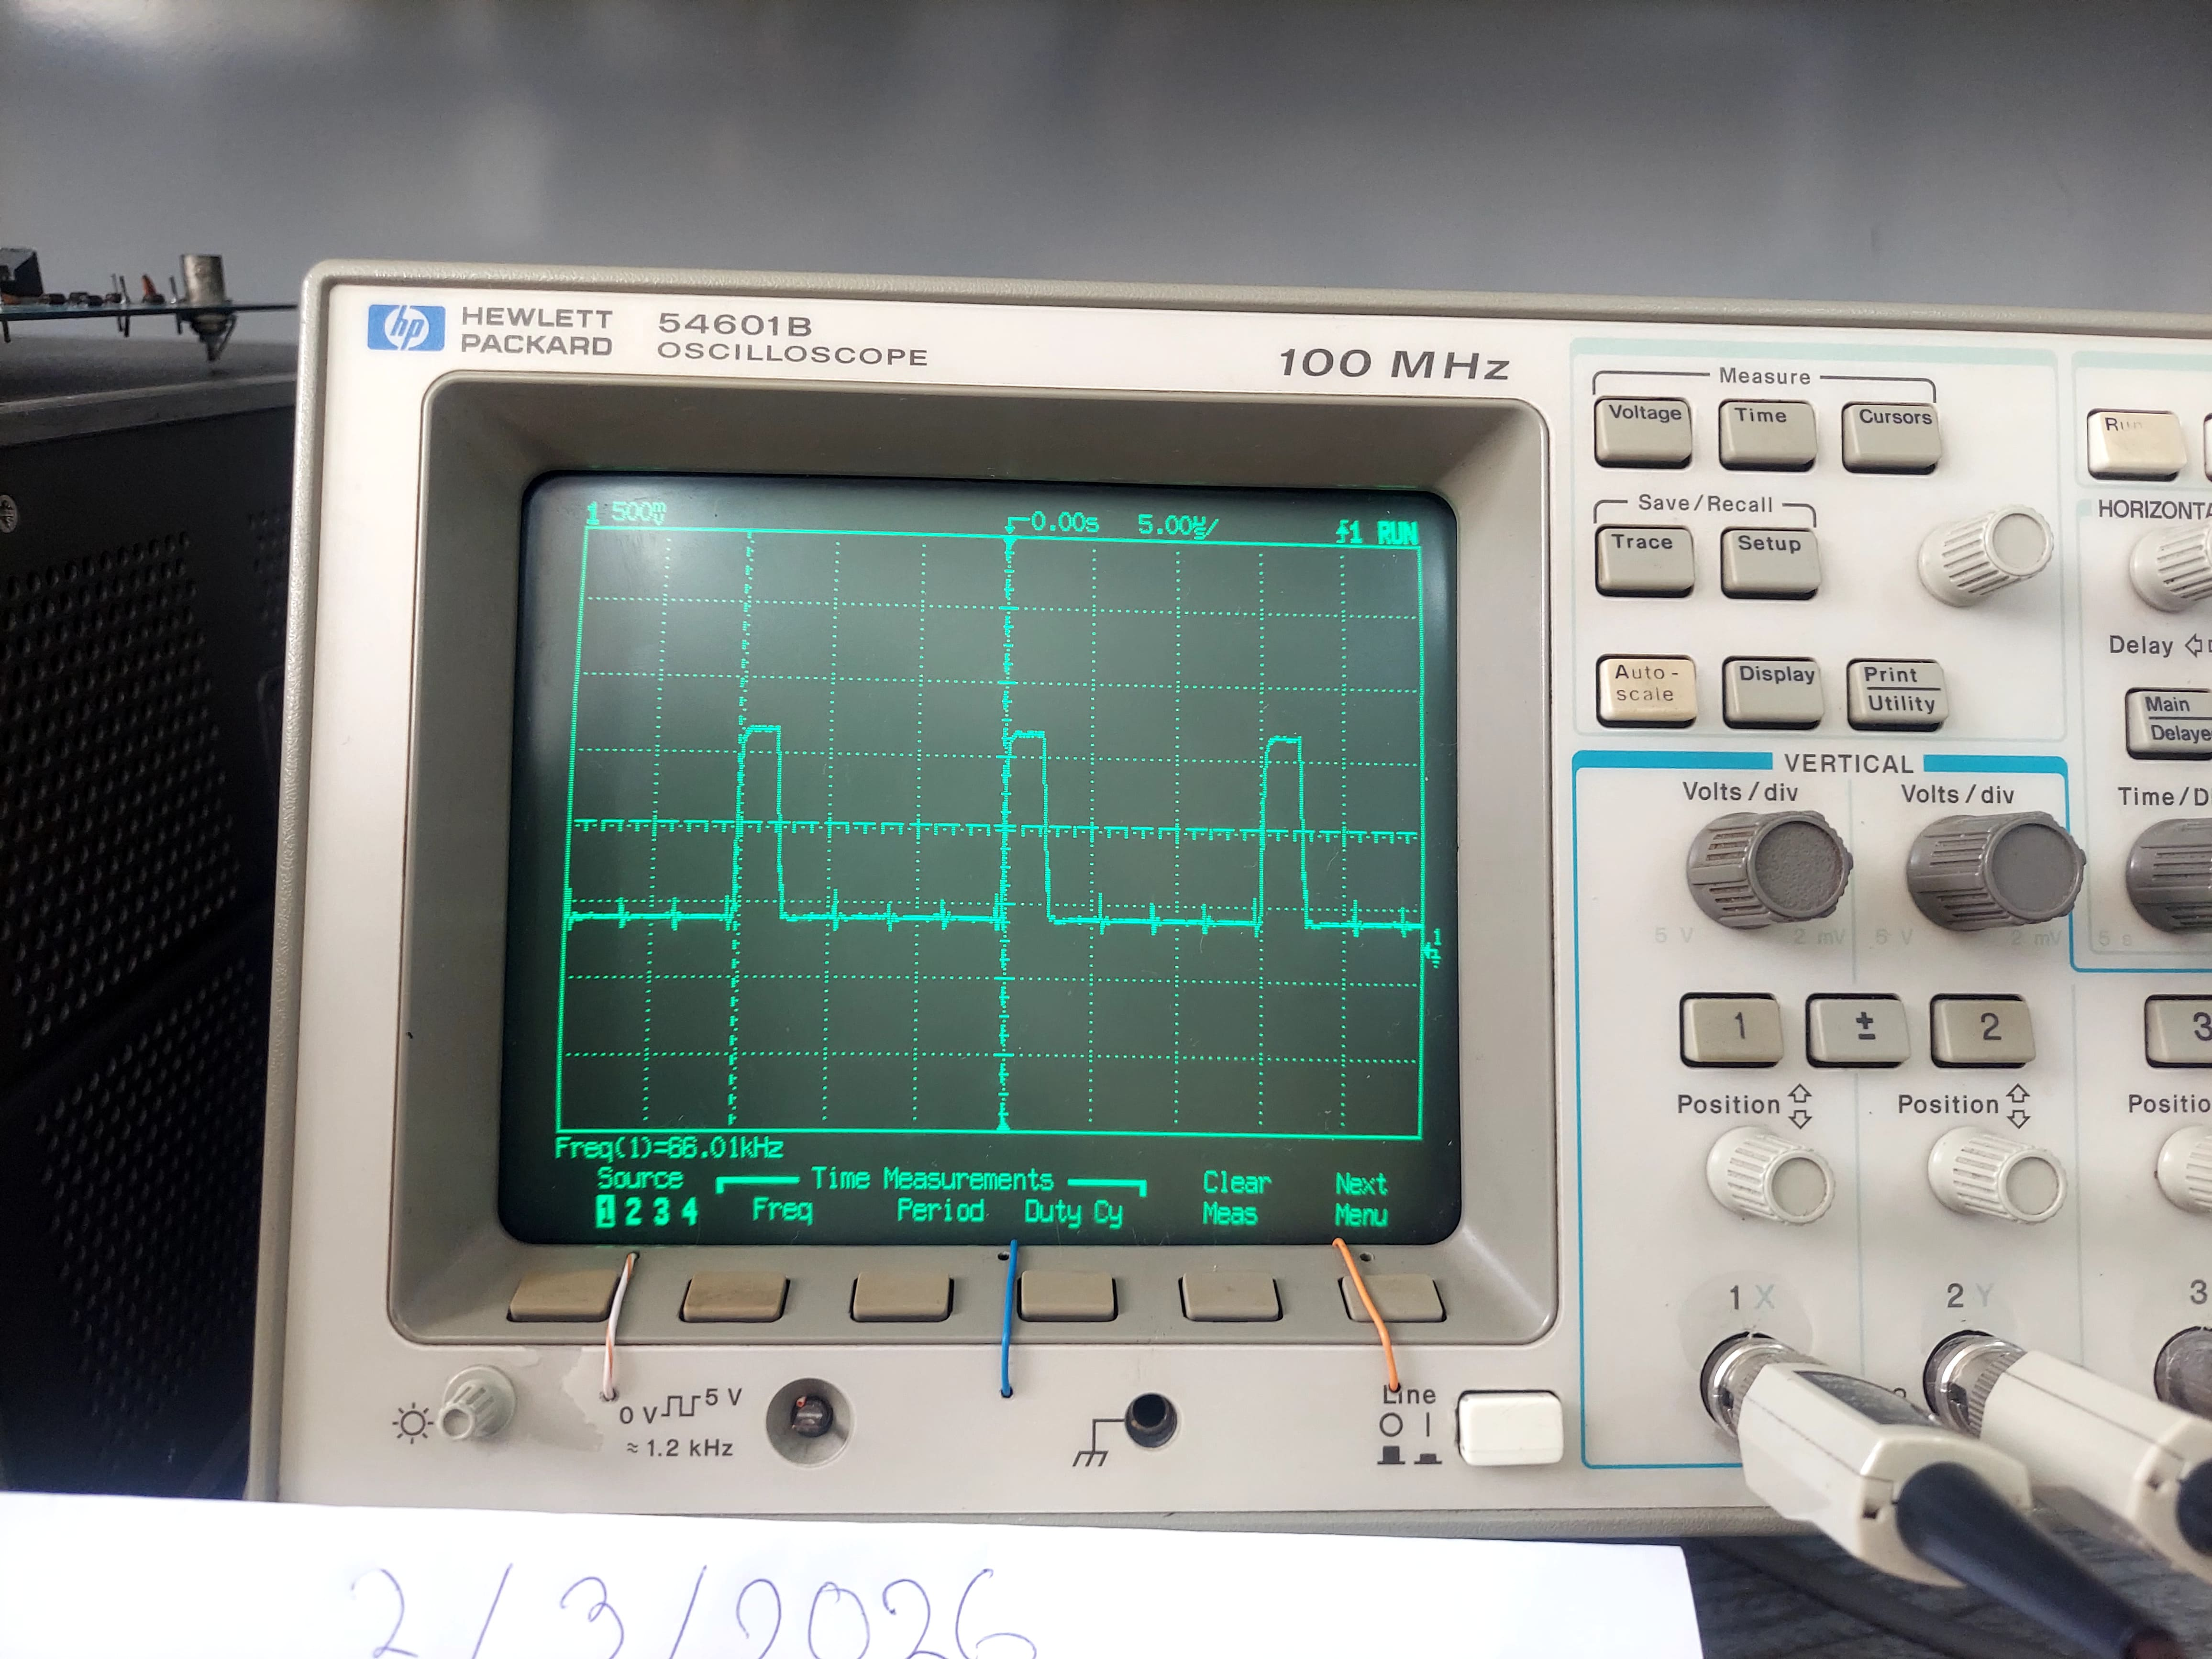
\includegraphics[width=\textwidth]{Imagenes/6-a.jpg}
        \caption{Señal multicanal A}
    \end{subfigure}
    \hfill
    \begin{subfigure}[b]{0.45\textwidth}
        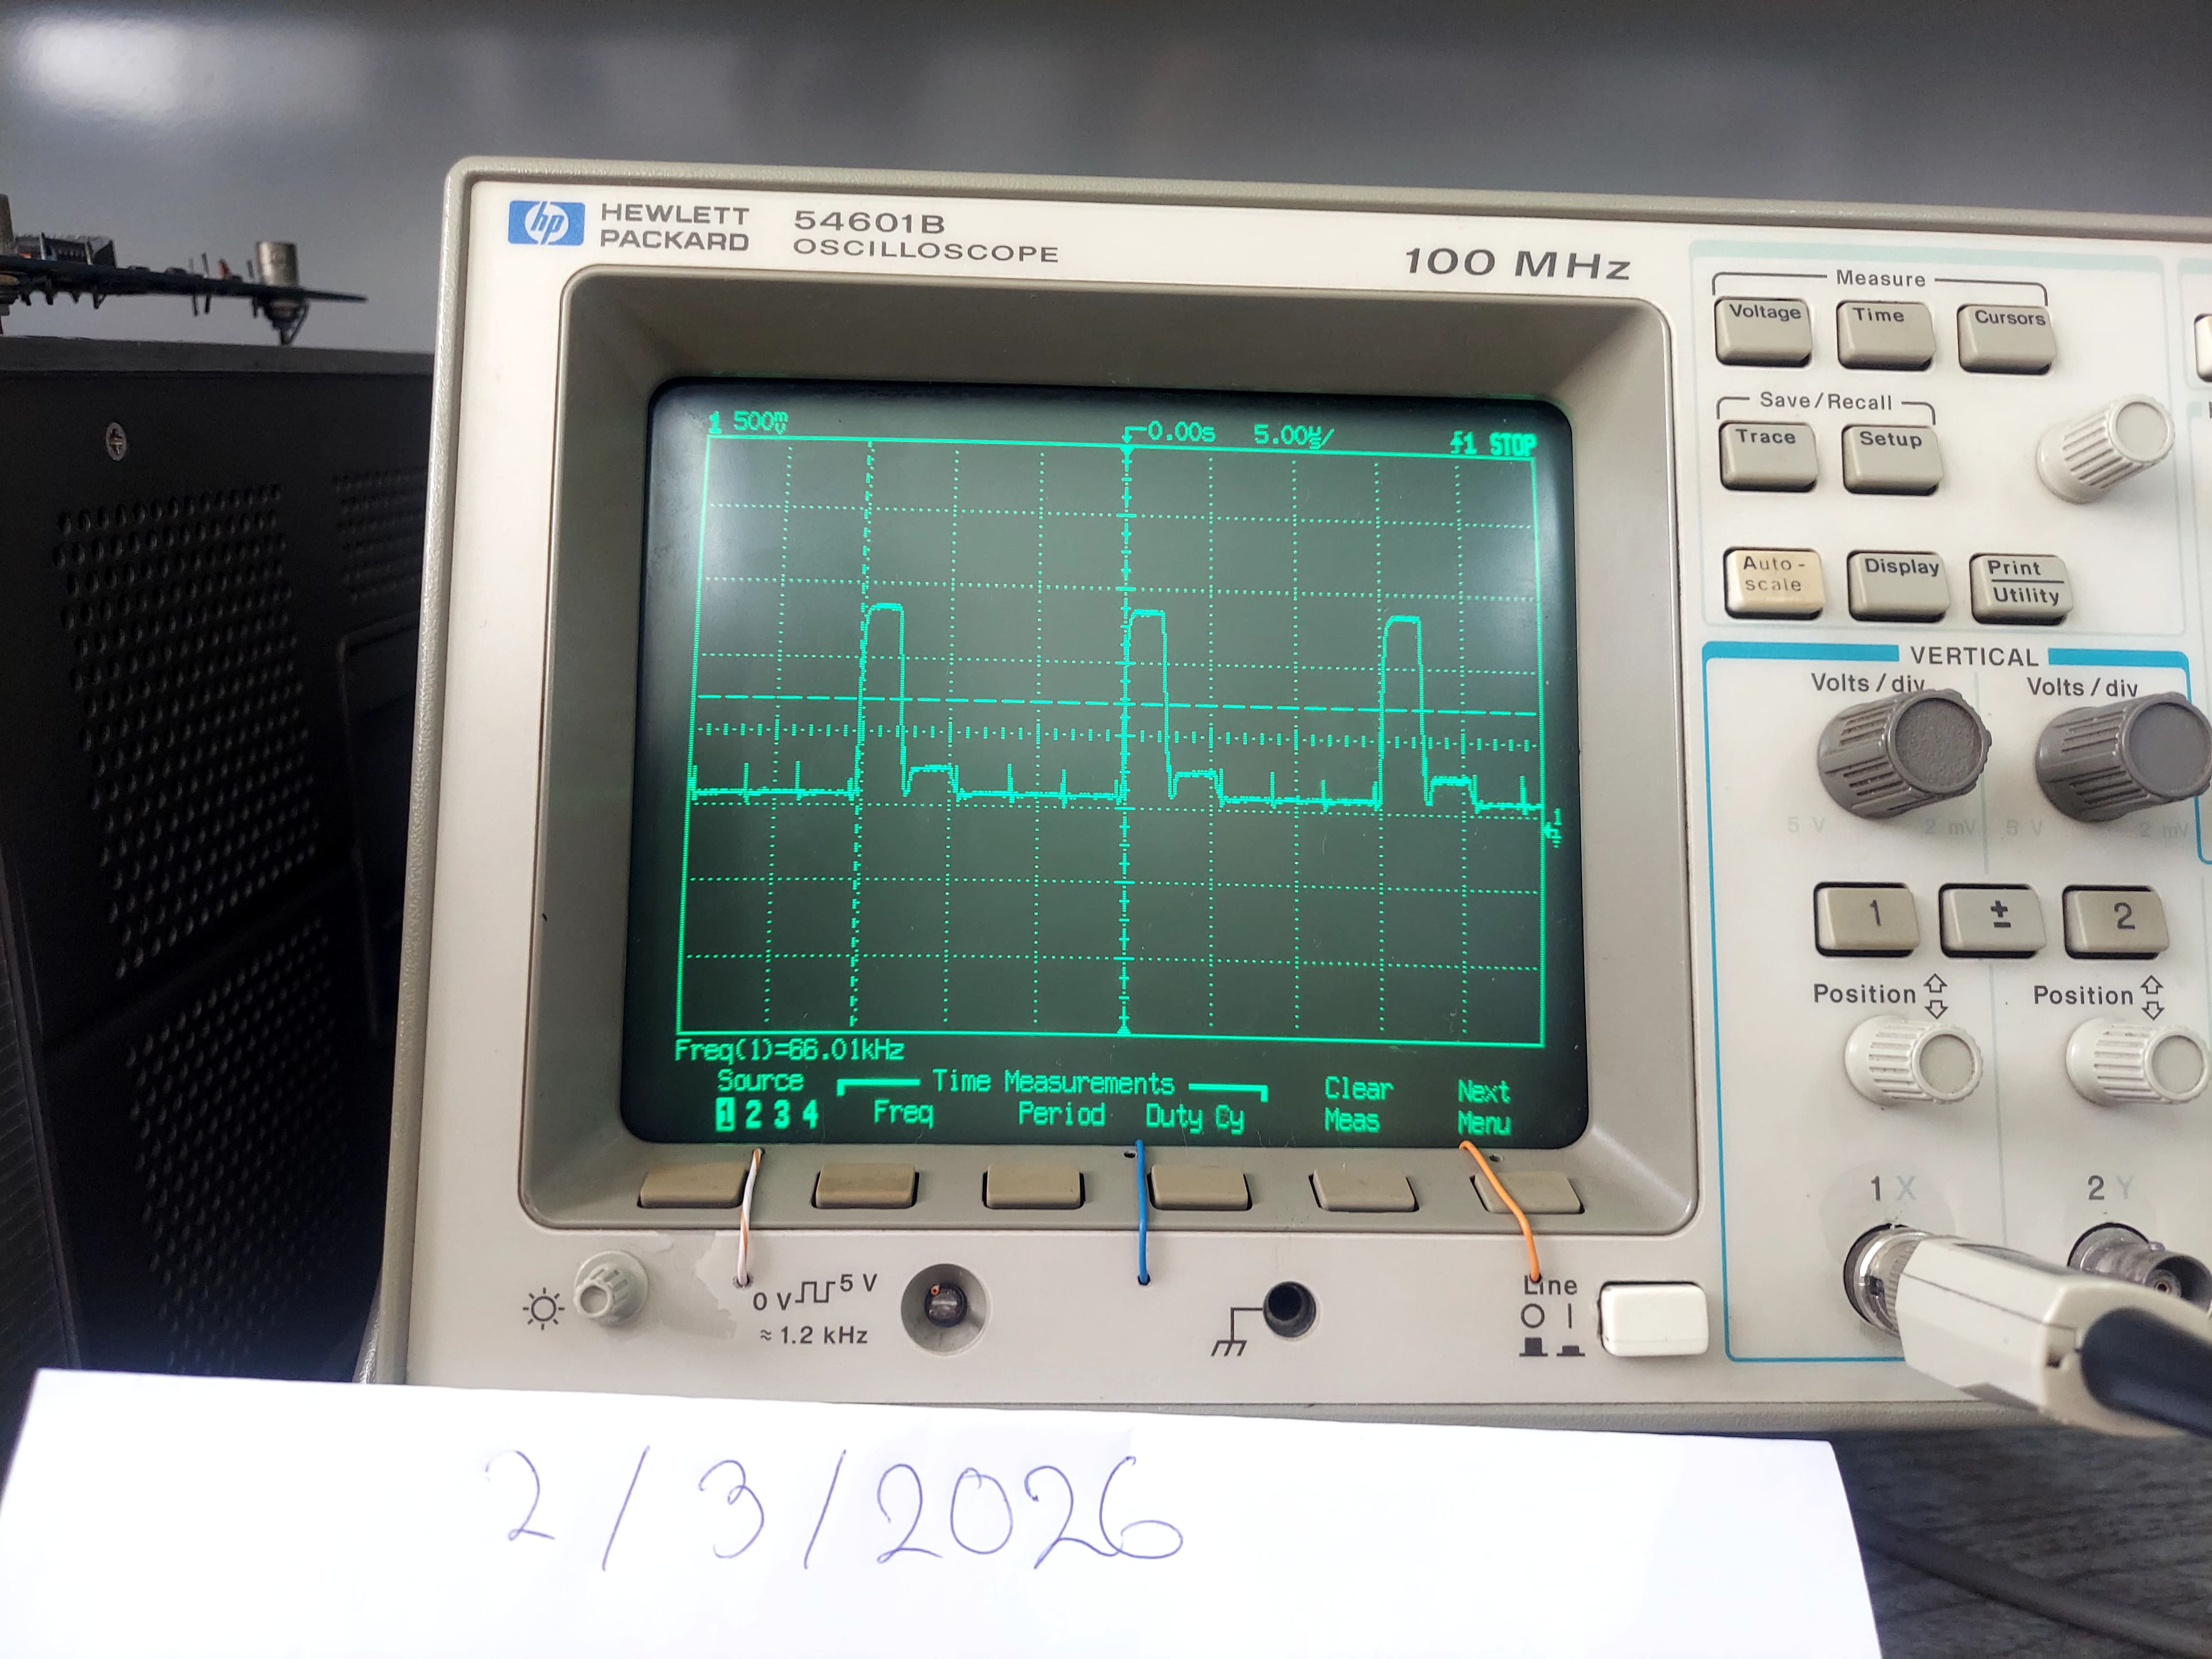
\includegraphics[width=\textwidth]{Imagenes/6-b.jpg}
        \caption{Señal multicanal B}
    \end{subfigure}
    \\[2ex]
    \begin{subfigure}[b]{0.45\textwidth}
        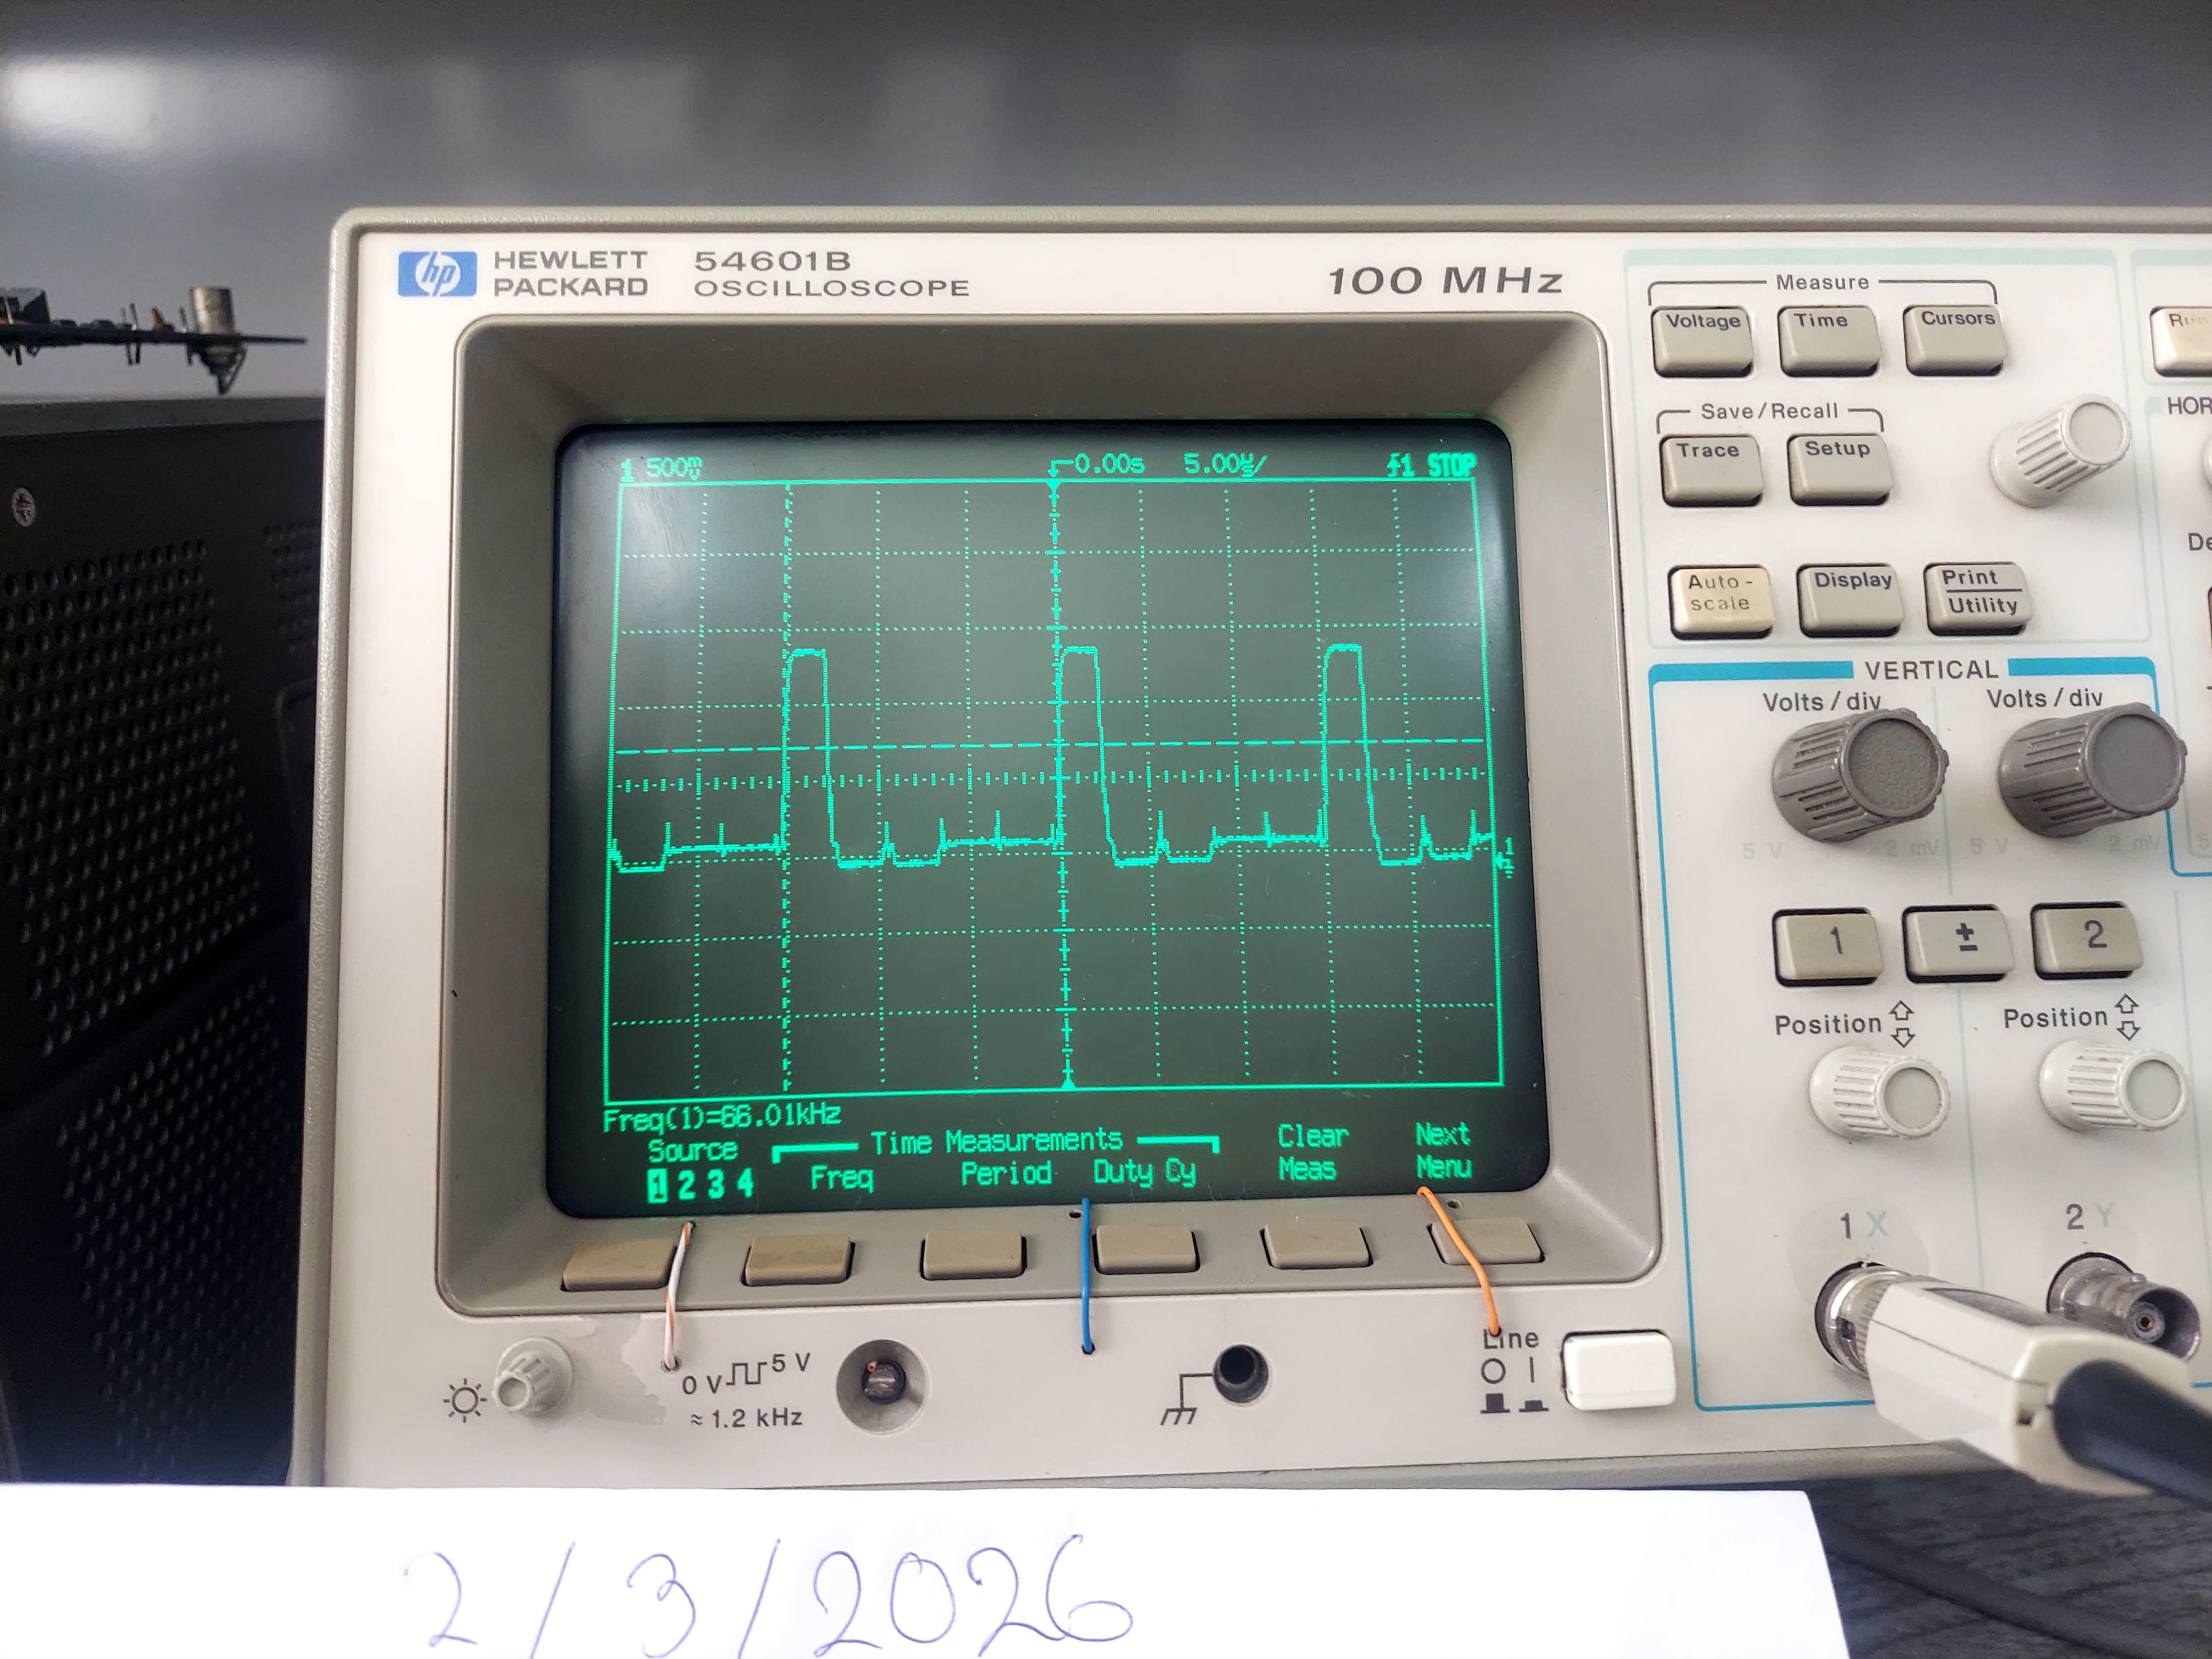
\includegraphics[width=\textwidth]{Imagenes/6-c.jpg}
        \caption{Señal multicanal C}
    \end{subfigure}
    \hfill
    \begin{subfigure}[b]{0.45\textwidth}
        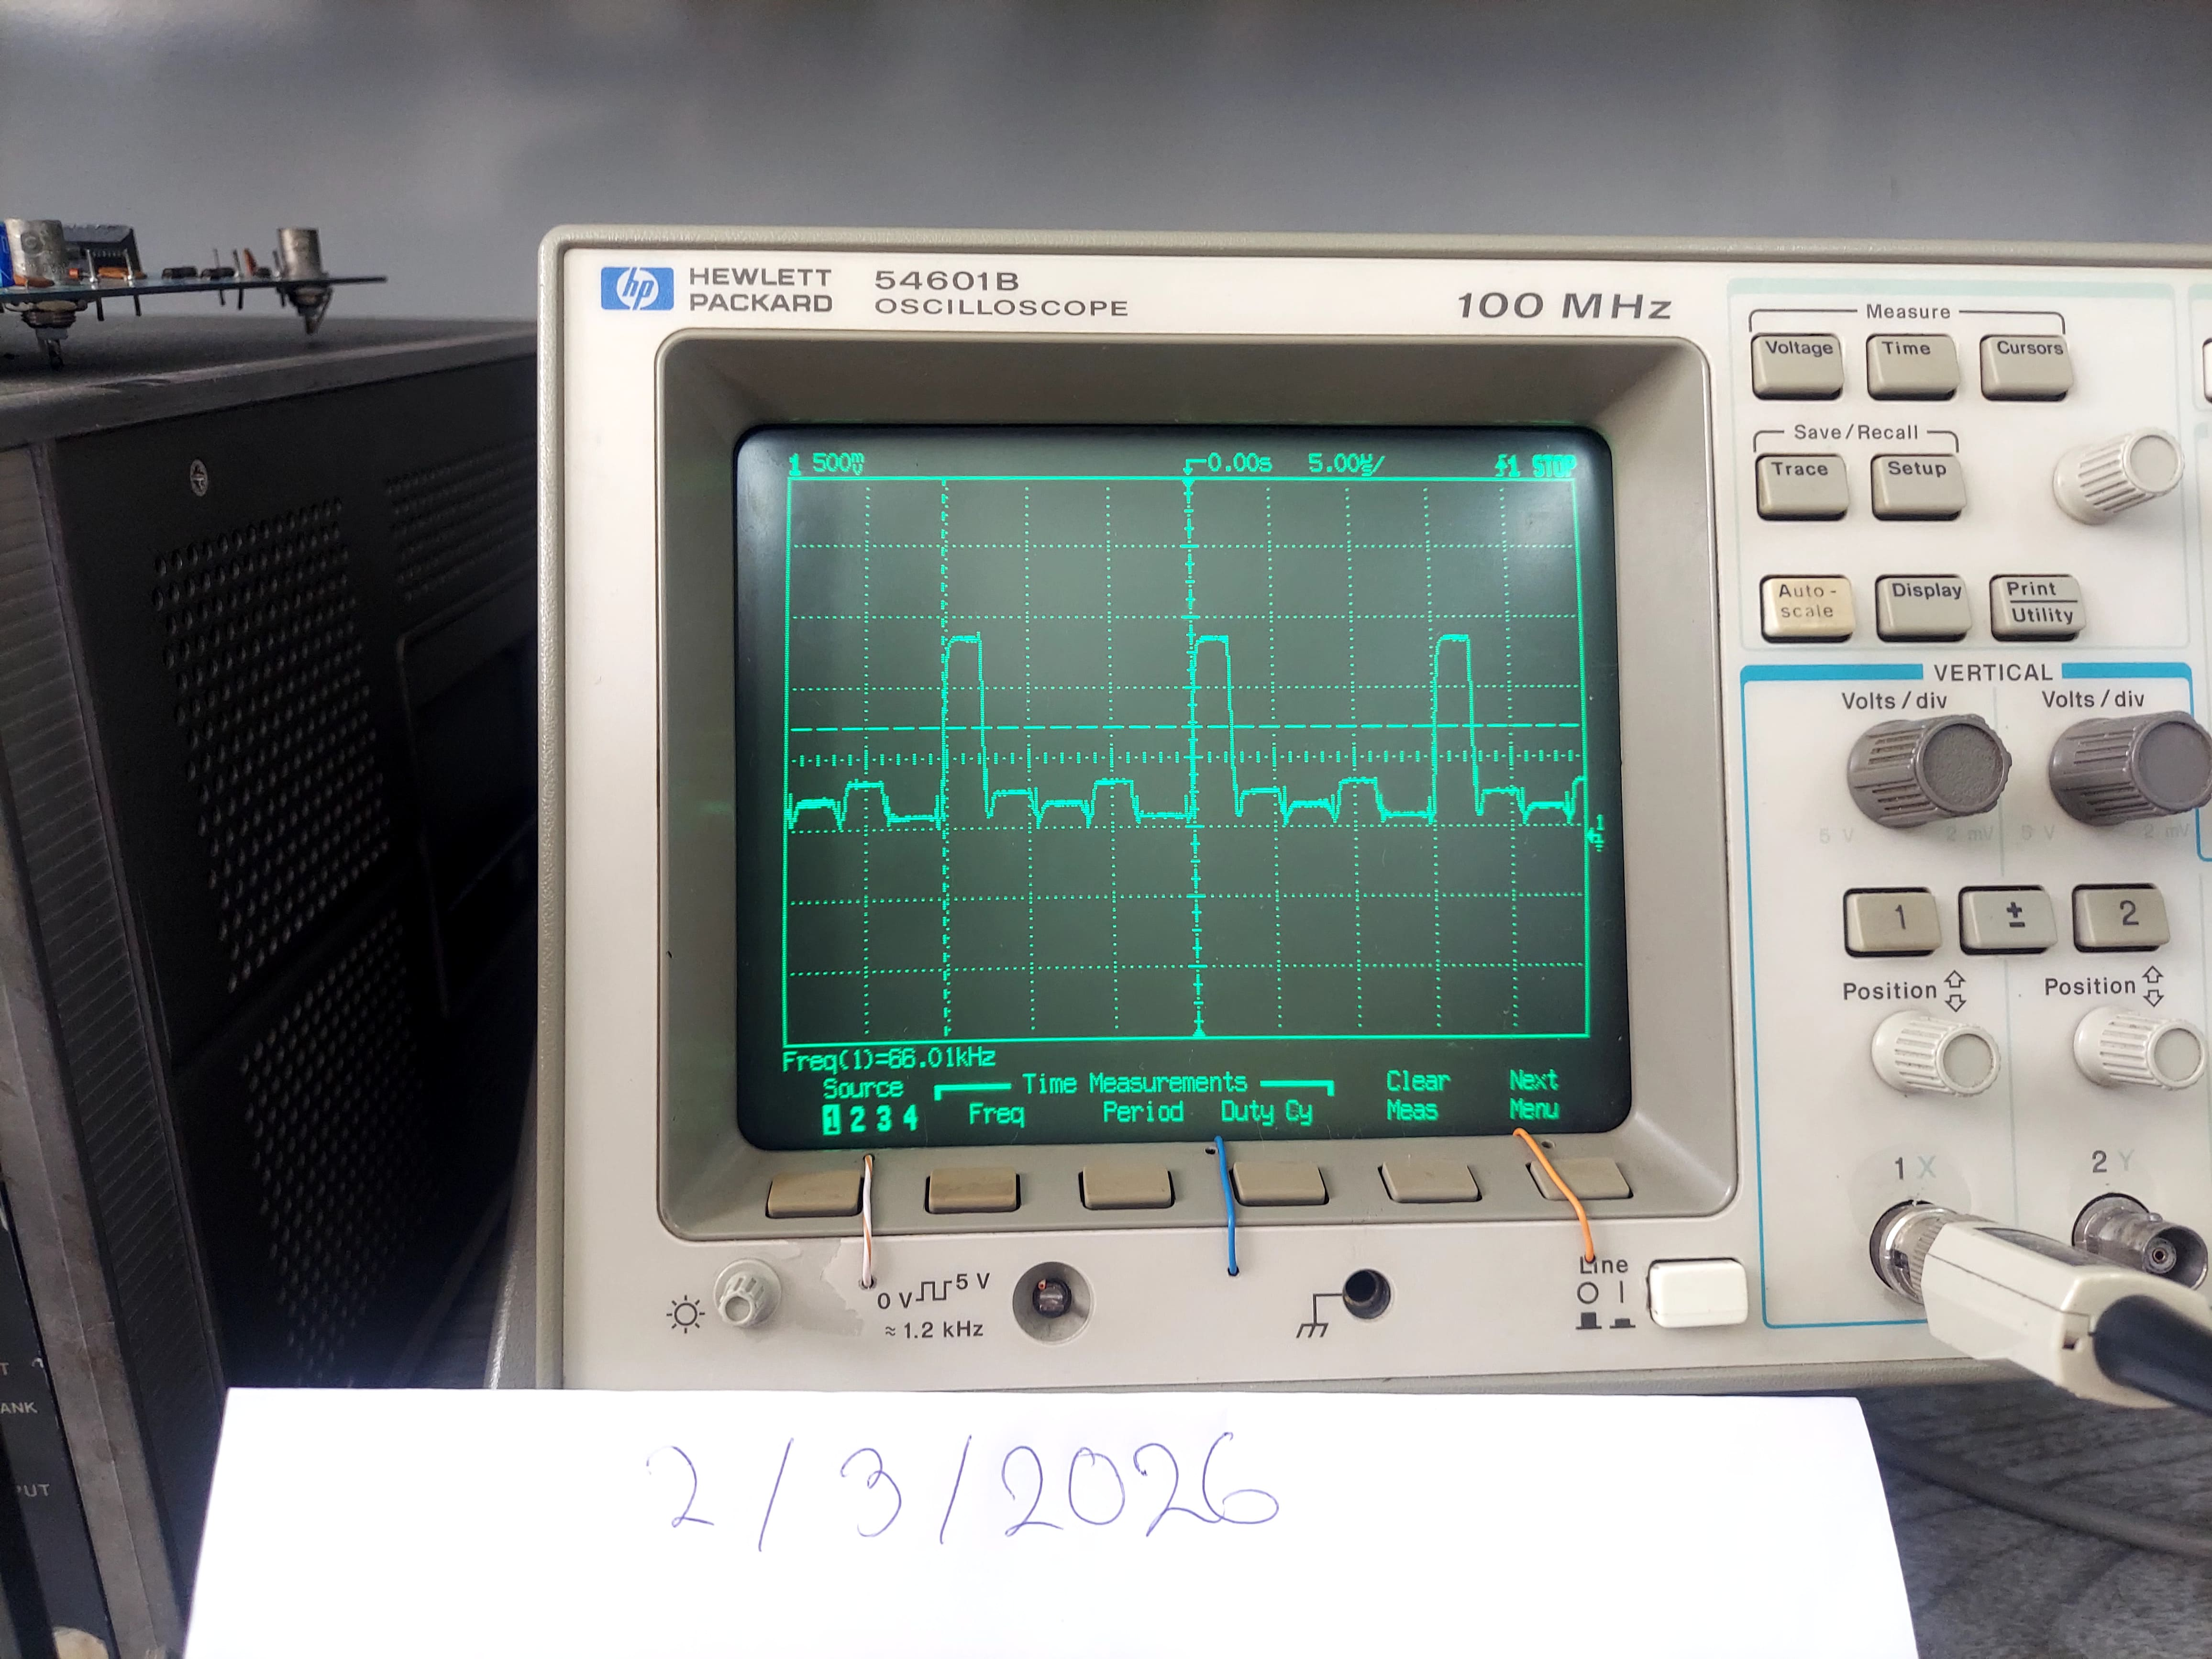
\includegraphics[width=\textwidth]{Imagenes/6-d.jpg}
        \caption{Señal multicanal D}
    \end{subfigure}
    \\[2ex]
    \begin{subfigure}[b]{0.45\textwidth}
        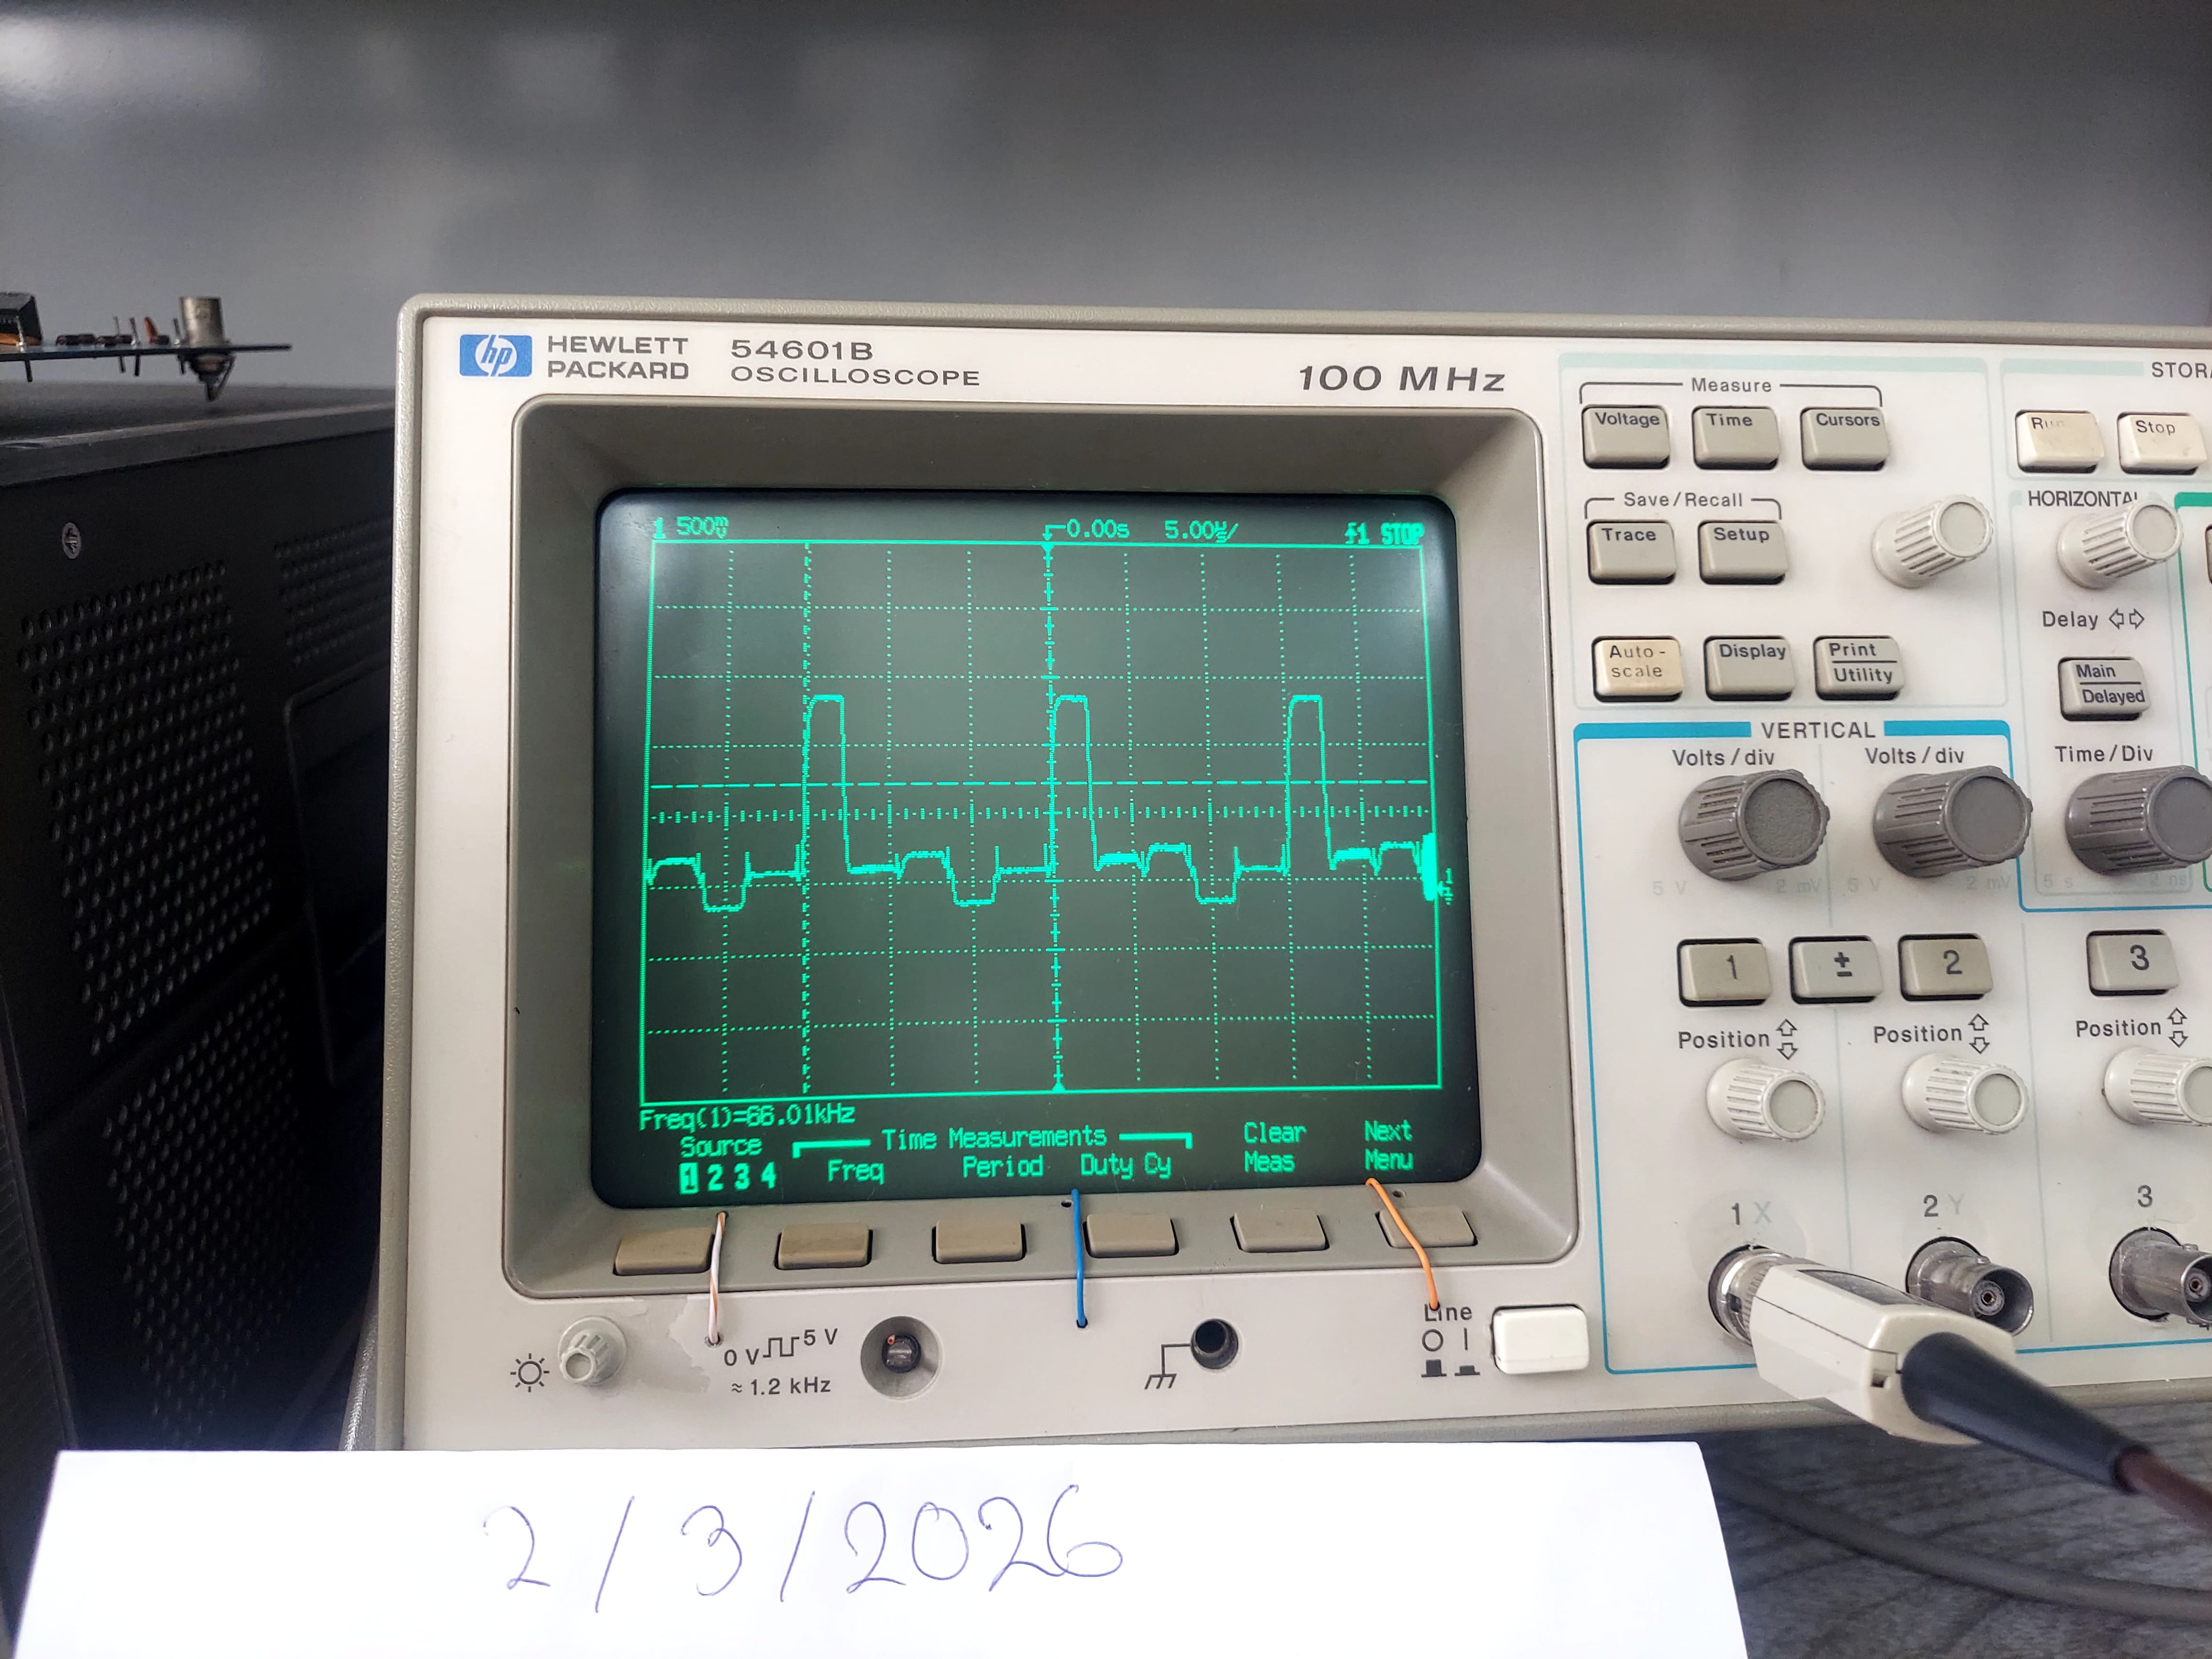
\includegraphics[width=\textwidth]{Imagenes/6-e.jpg}
        \caption{Señal multicanal E}
    \end{subfigure}
    \caption{Identificación de canales y señal de sincronismo en TP9.}
\end{figure}

\subsection{Paso 7: Transmisión en Banda Base}
\textbf{Instrucciones:} Coloque el conmutador en la posición "BNC" y una la sección de transmisión con la de recepción por medio de un cable coaxial. Observe las señales recibidas en el punto TP11 (señal multicanal recibida), 1, 2, 3 y 4 (señales detectadas de cada canal). Escuche las señales recuperadas por medio del amplificador de audio y la corneta interna.

\begin{figure}[H]
    \centering
    \begin{subfigure}[b]{0.45\textwidth}
        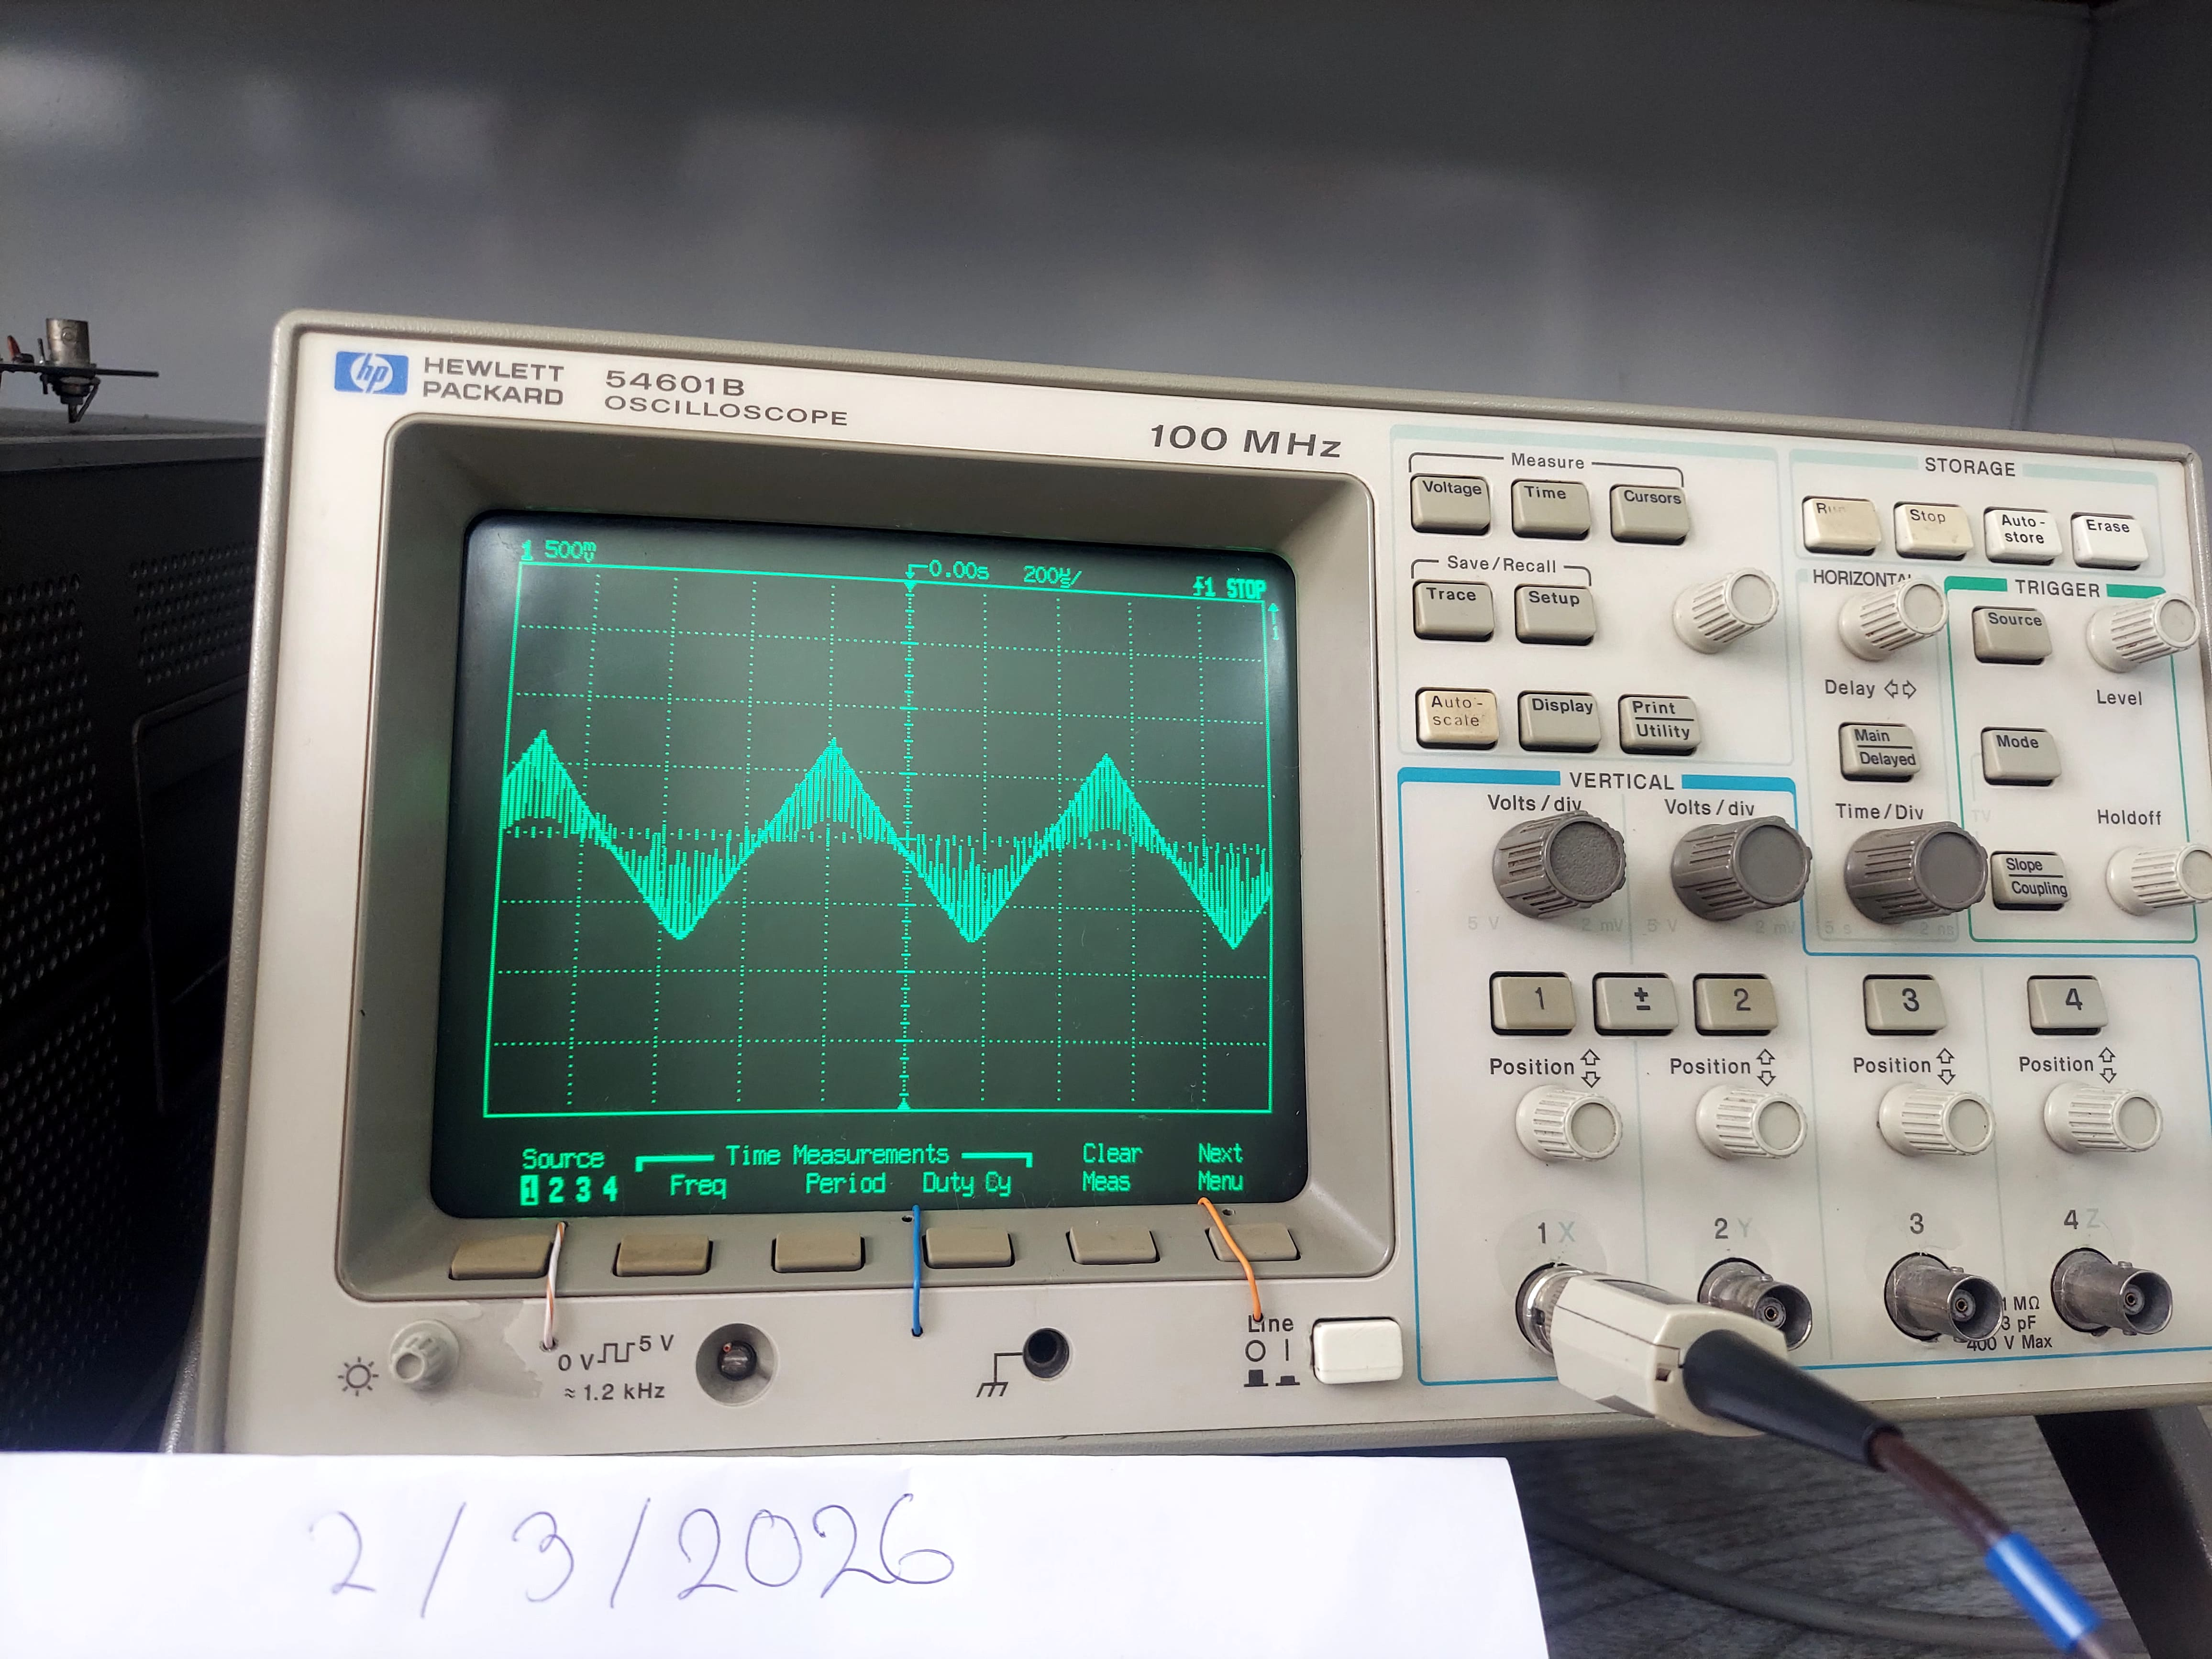
\includegraphics[width=\textwidth]{Imagenes/7-a.jpg}
        \caption{Señal recibida A}
    \end{subfigure}
    \hfill
    \begin{subfigure}[b]{0.45\textwidth}
        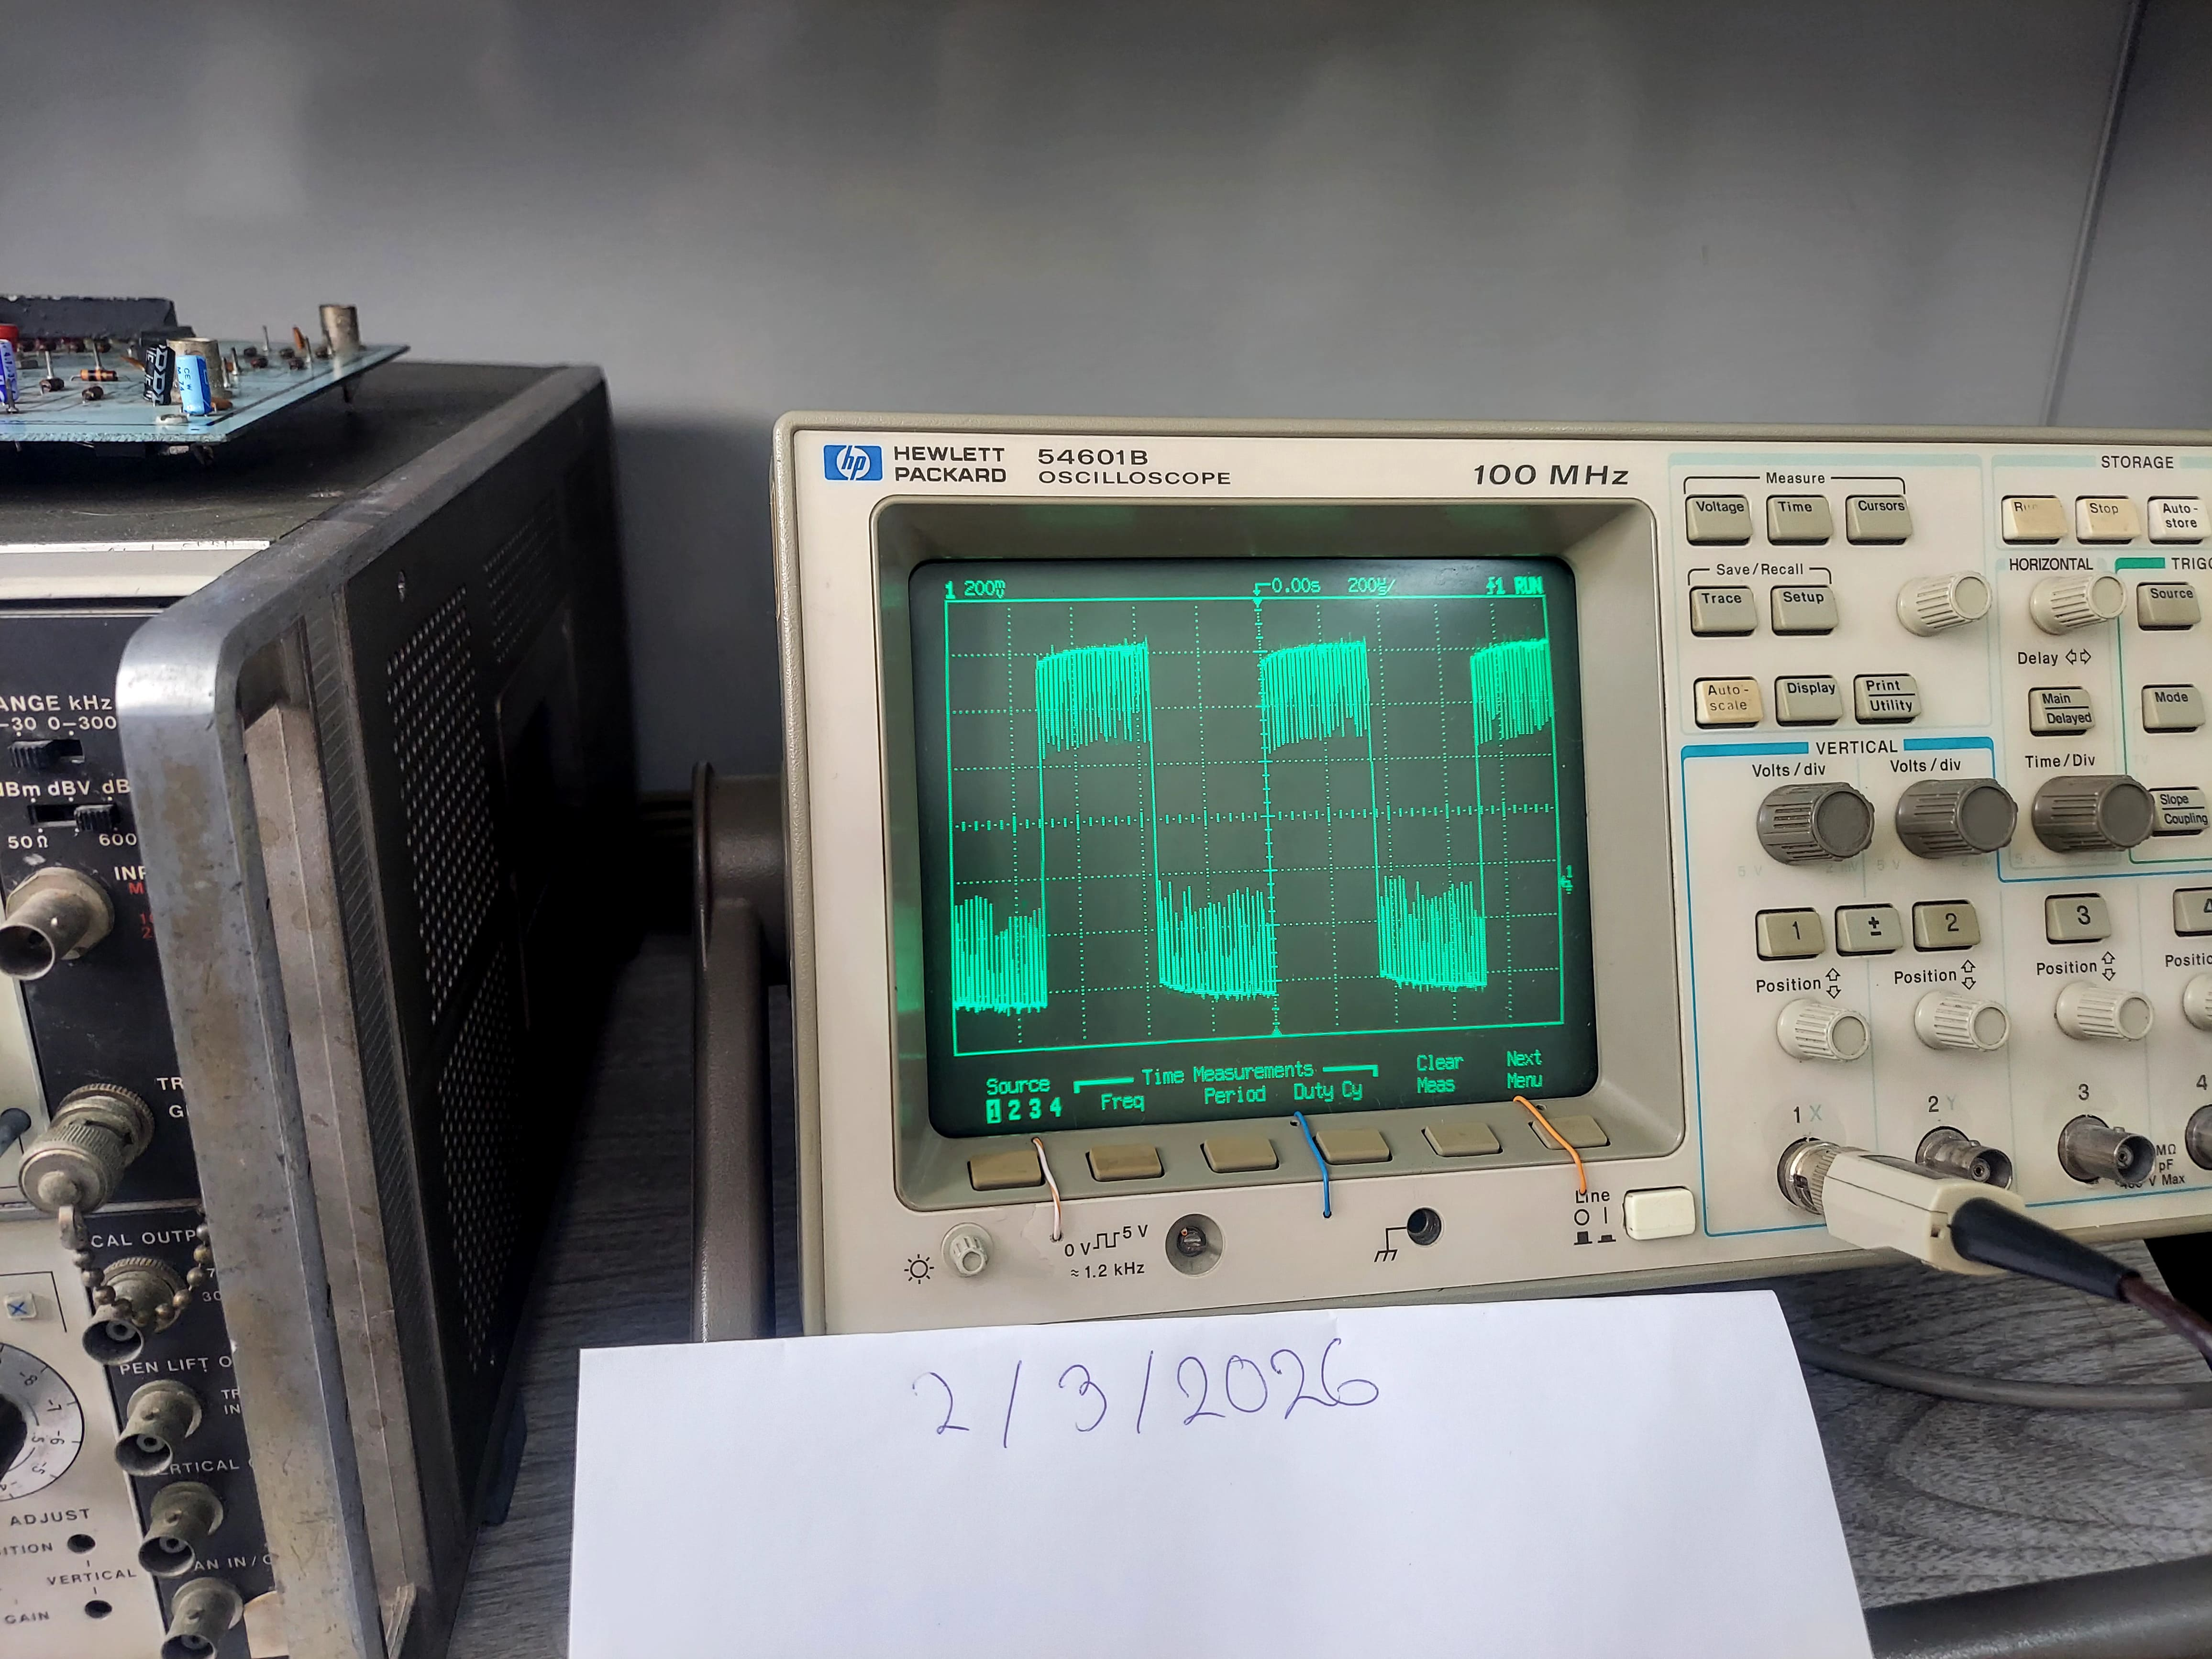
\includegraphics[width=\textwidth]{Imagenes/7-b.jpg}
        \caption{Señal recibida B}
    \end{subfigure}
    \\[2ex]
    \begin{subfigure}[b]{0.45\textwidth}
        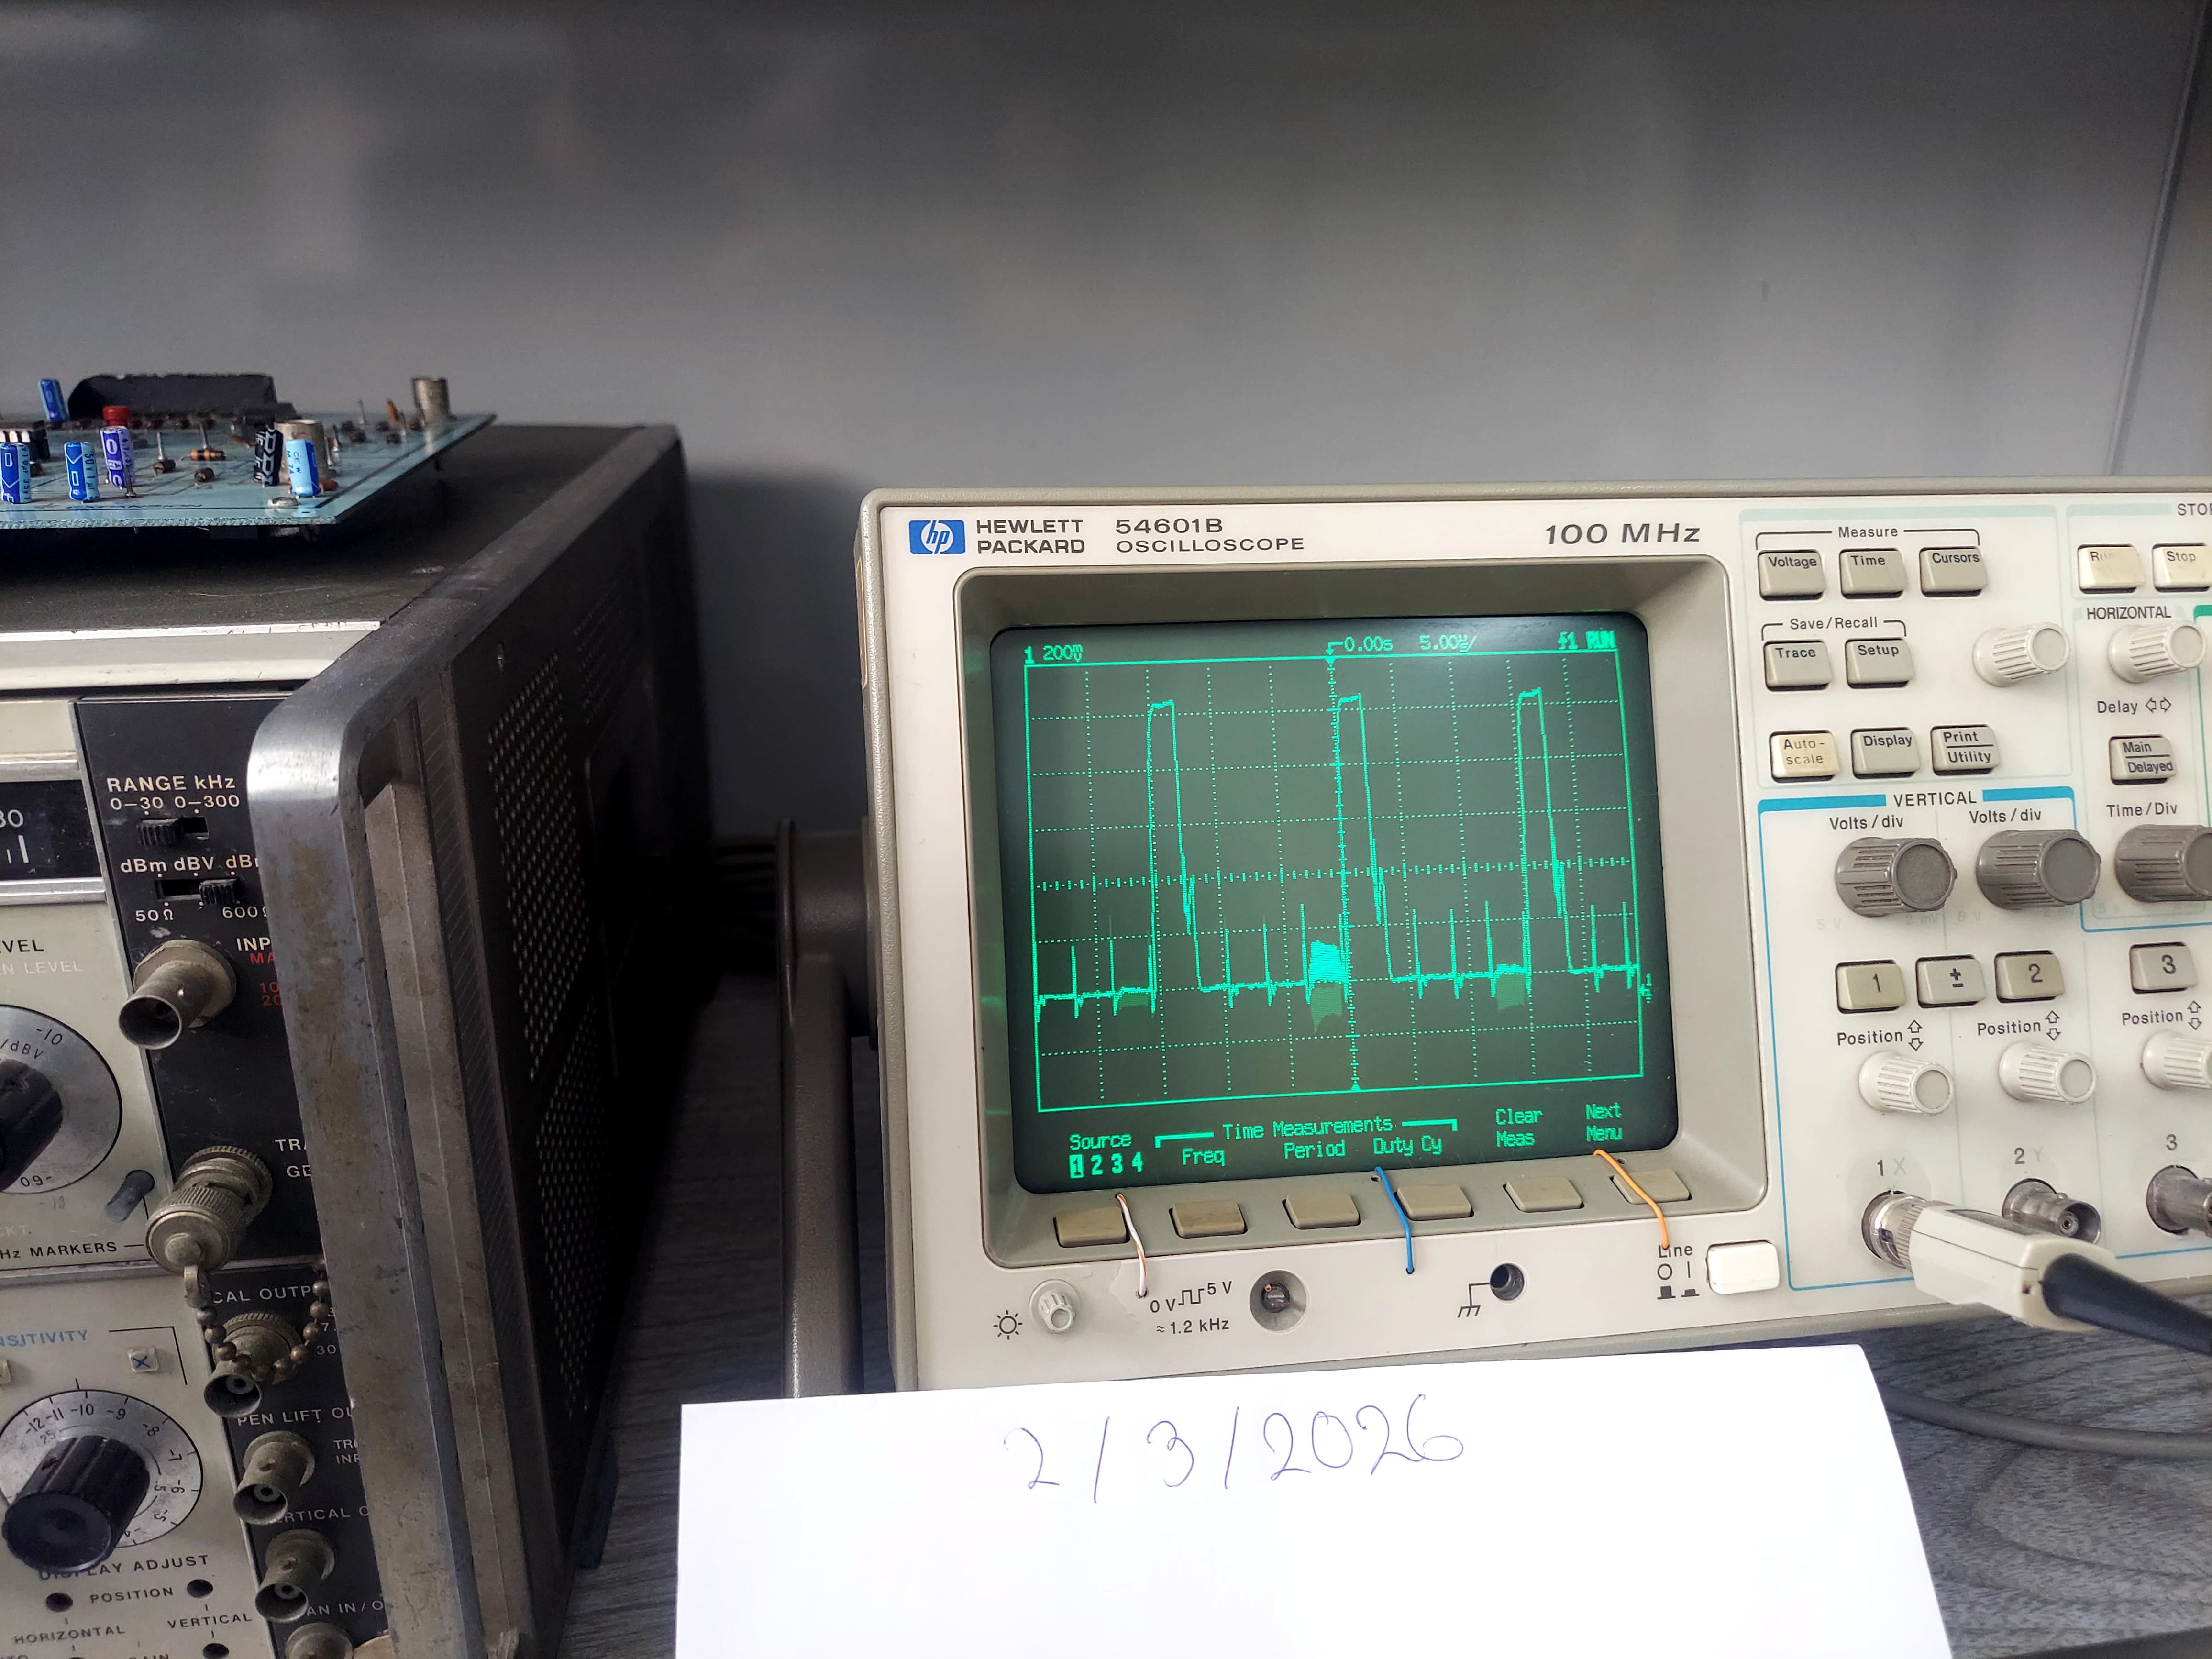
\includegraphics[width=\textwidth]{Imagenes/7-c.jpg}
        \caption{Señal recibida C}
    \end{subfigure}
    \caption{Señales recibidas en TP11 y detección de canales.}
\end{figure}

\subsection{Paso 8: Recuperación del Reloj y del Sincronismo}
\textbf{Instrucciones:}
\begin{itemize}
    \item Coloque el canal A del osciloscopio en el punto TP8 y el canal B en el TP12. Observe la señal de reloj recuperada: ésta es la salida del VCO del circuito P.L.L. NE565. Observe las señales en el osciloscopio a medida que varía el control CLOCK ADJ.
    \item Solo con el puente No. 1 conectado, escuche las señales en los puntos 1, 2, 3 y 4 de recepción para varios ajustes de control exterior. Explique a que se deben los efectos observados. Reajuste el CLOCK ADJ. hasta obtener la señal únicamente en la salida "1" del receptor. Investigue sobre el funcionamiento de este circuito recuperador de reloj.
\end{itemize}

\begin{figure}[H]
    \centering
    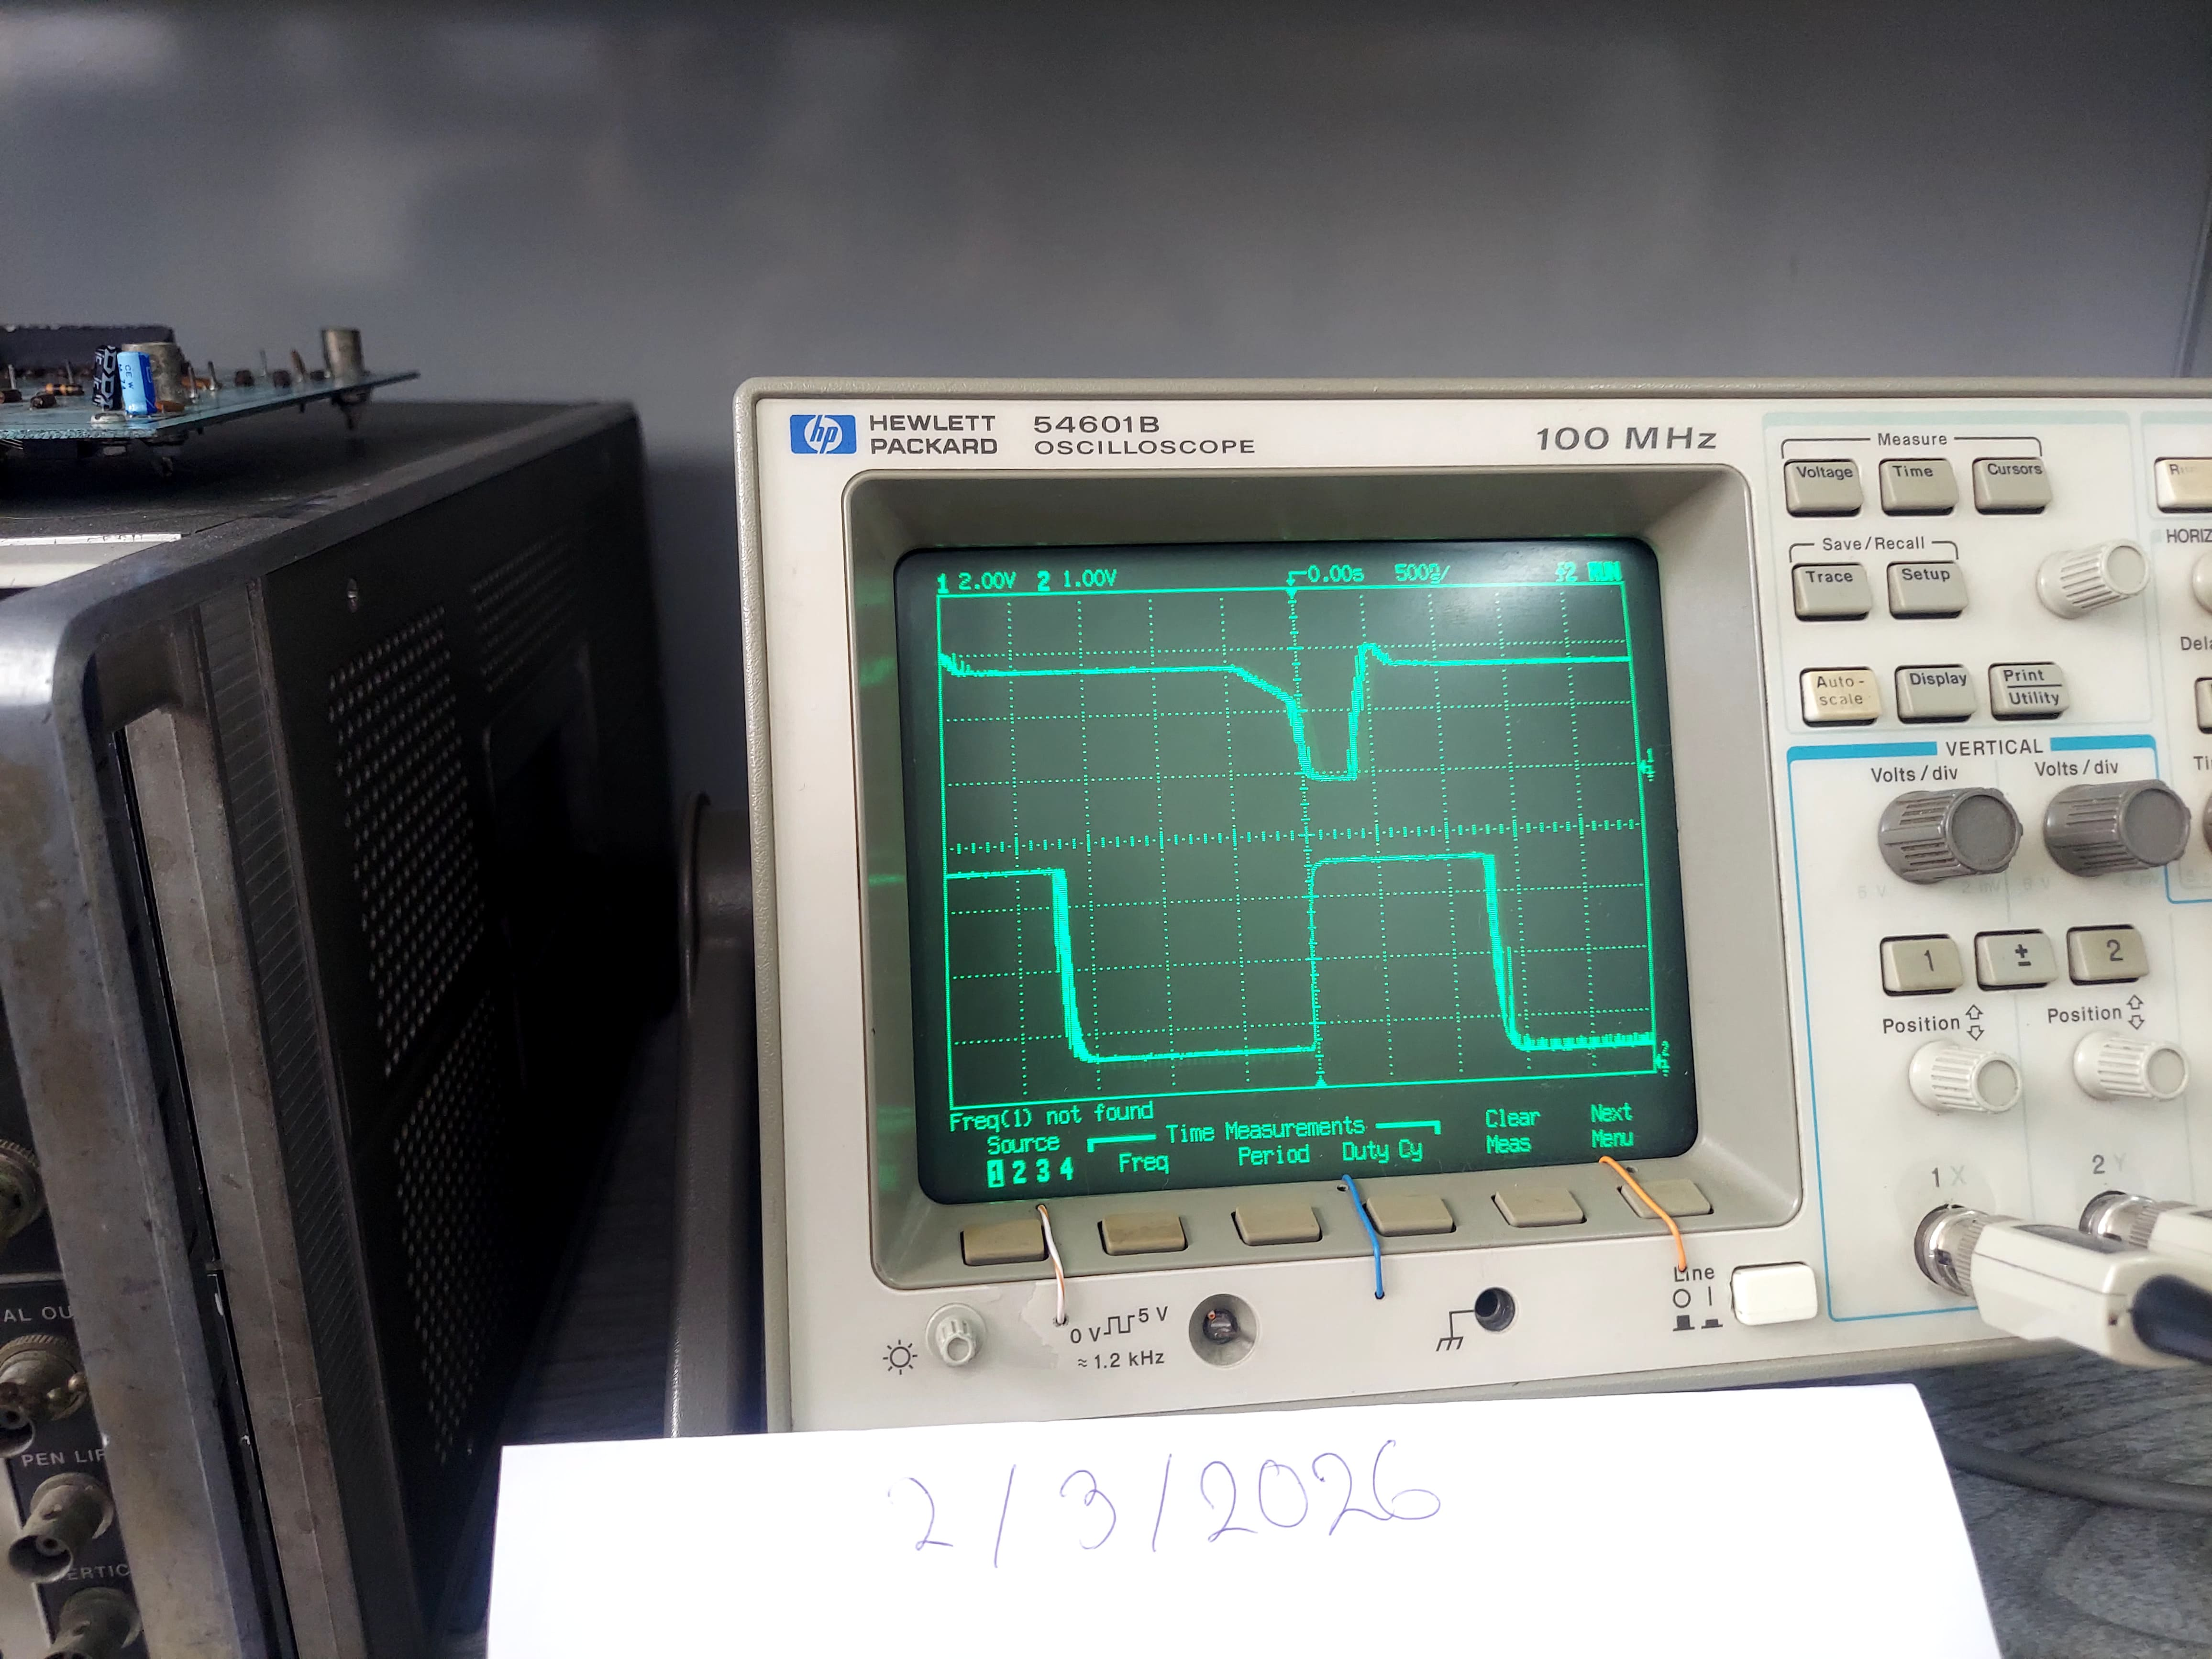
\includegraphics[width=0.8\textwidth]{Imagenes/8-sin-ajuste.jpg}
    \caption{Señal sin ajuste de reloj}
\end{figure}

\begin{figure}[H]
    \centering
    \begin{subfigure}[b]{0.45\textwidth}
        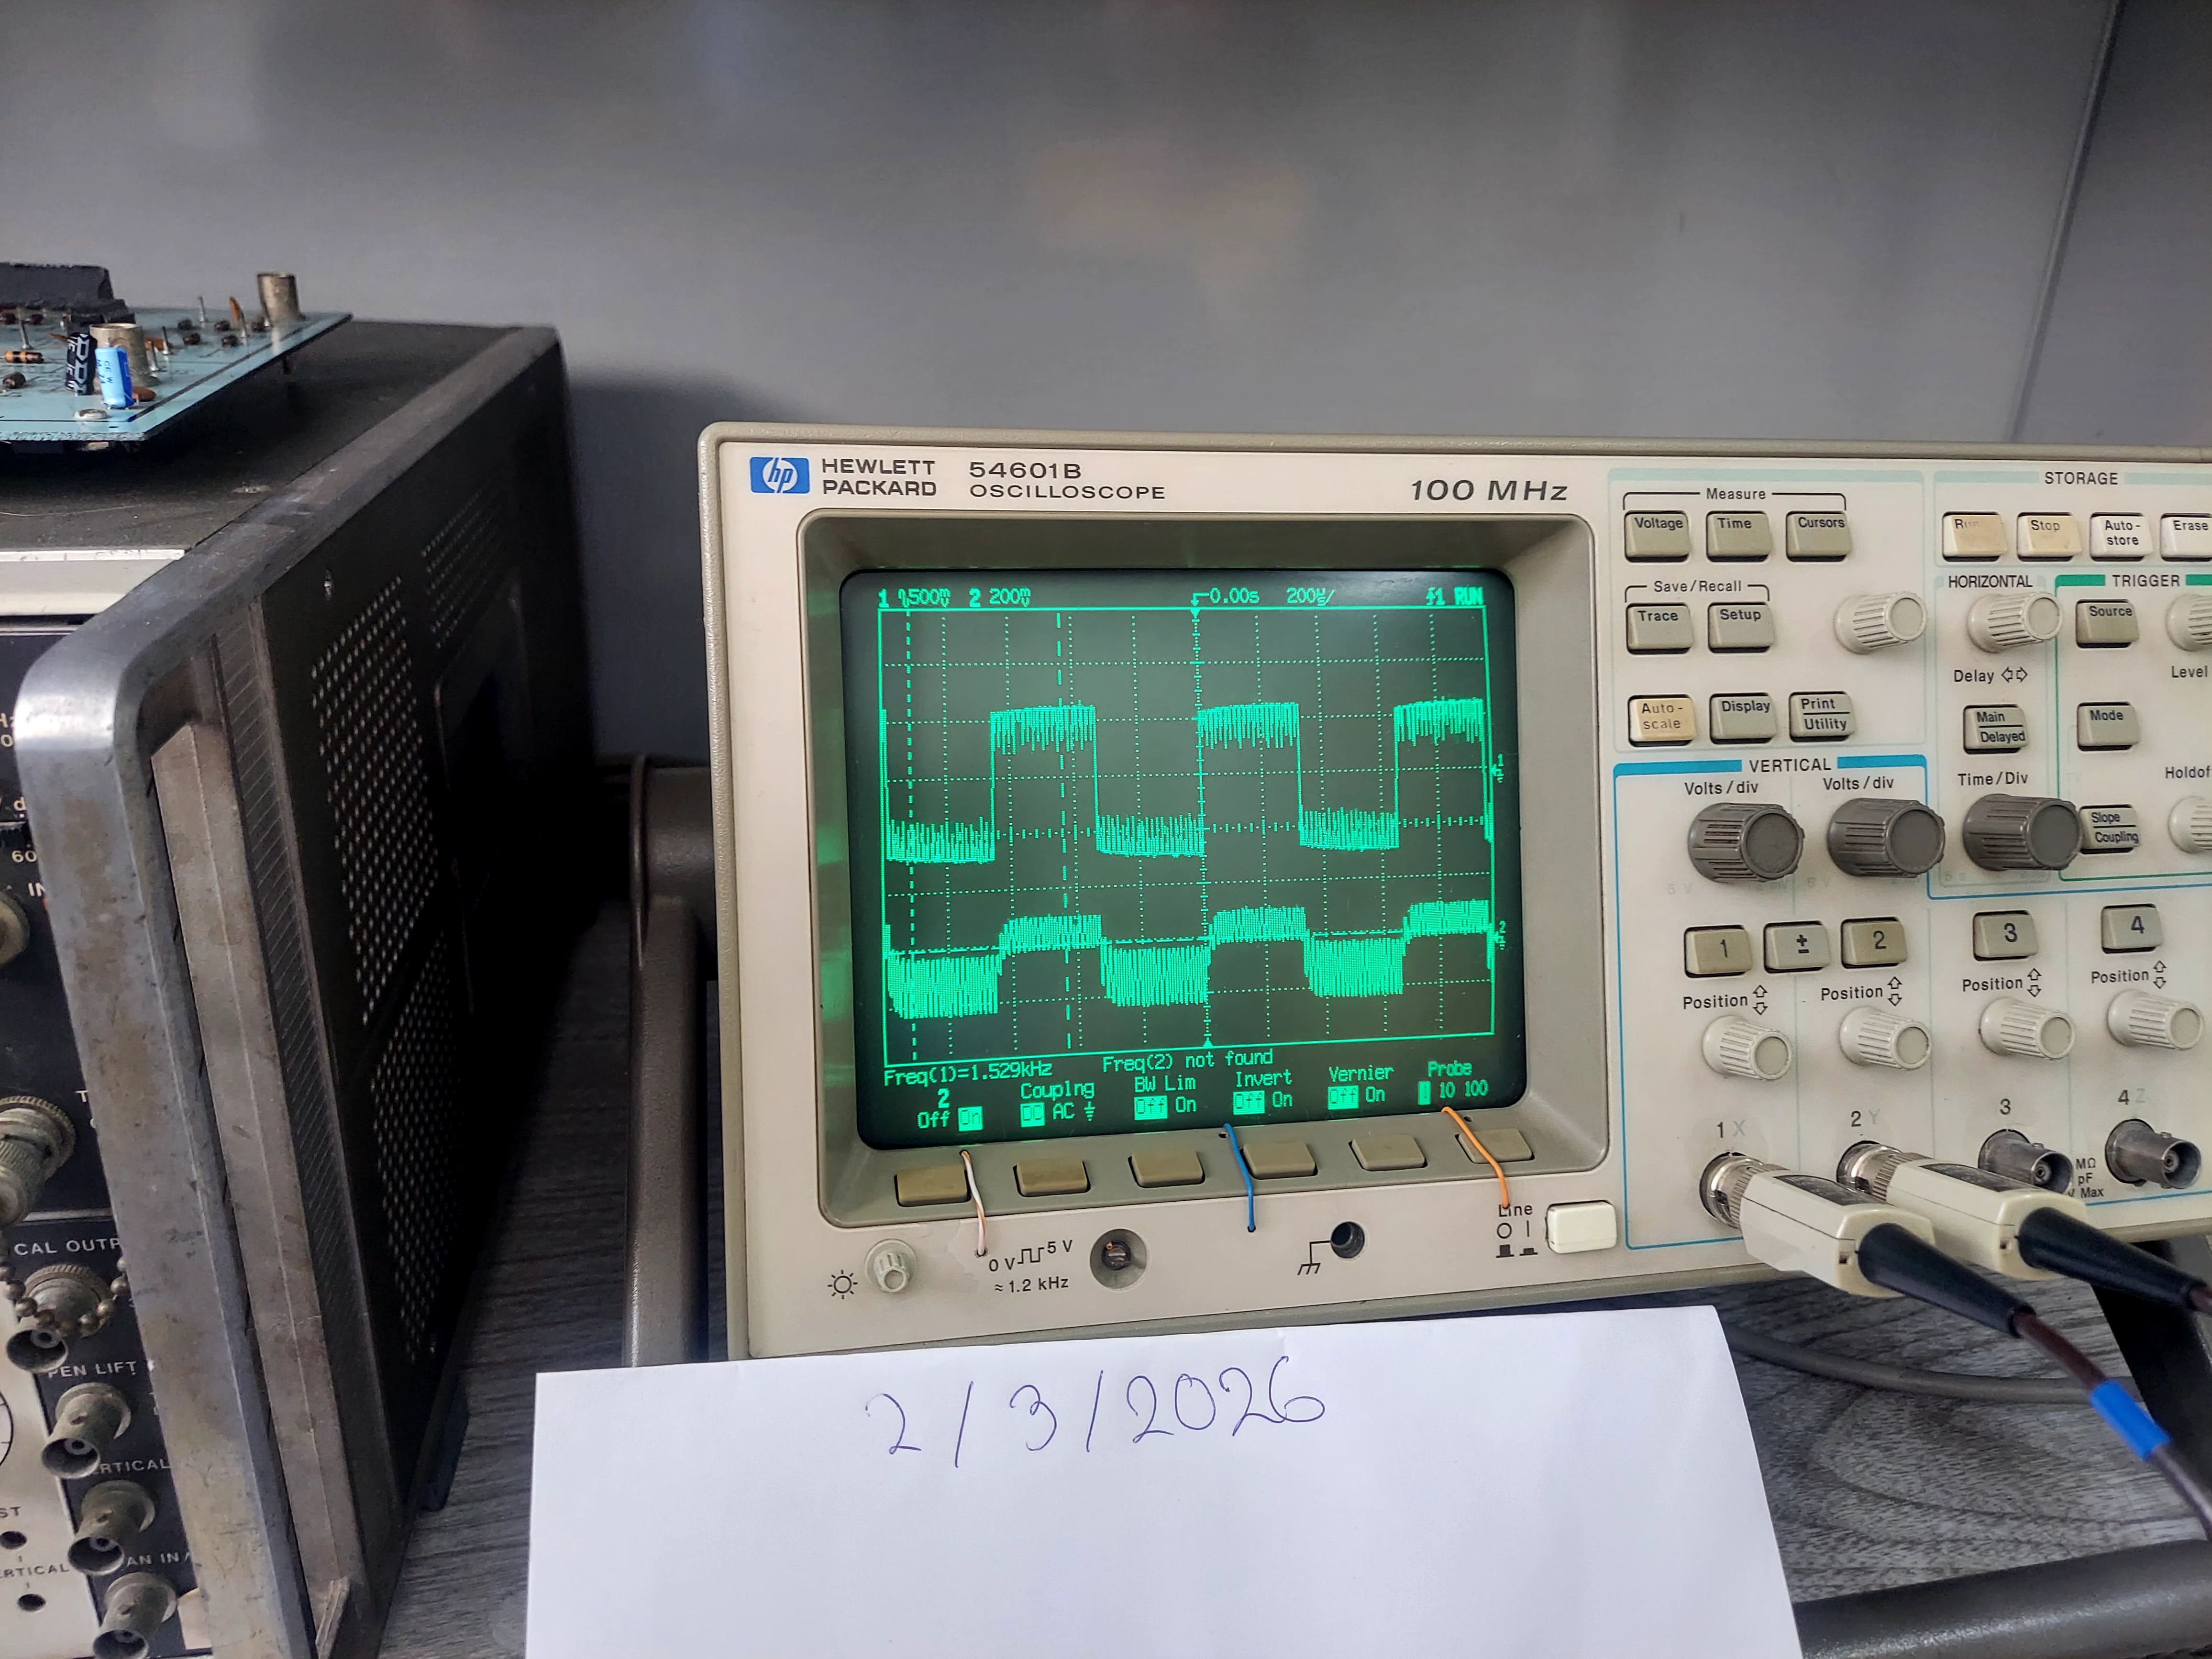
\includegraphics[width=\textwidth]{Imagenes/8-cuadrada-bien.jpg}
        \caption{Señal cuadrada ajustada}
    \end{subfigure}
    \hfill
    \begin{subfigure}[b]{0.45\textwidth}
        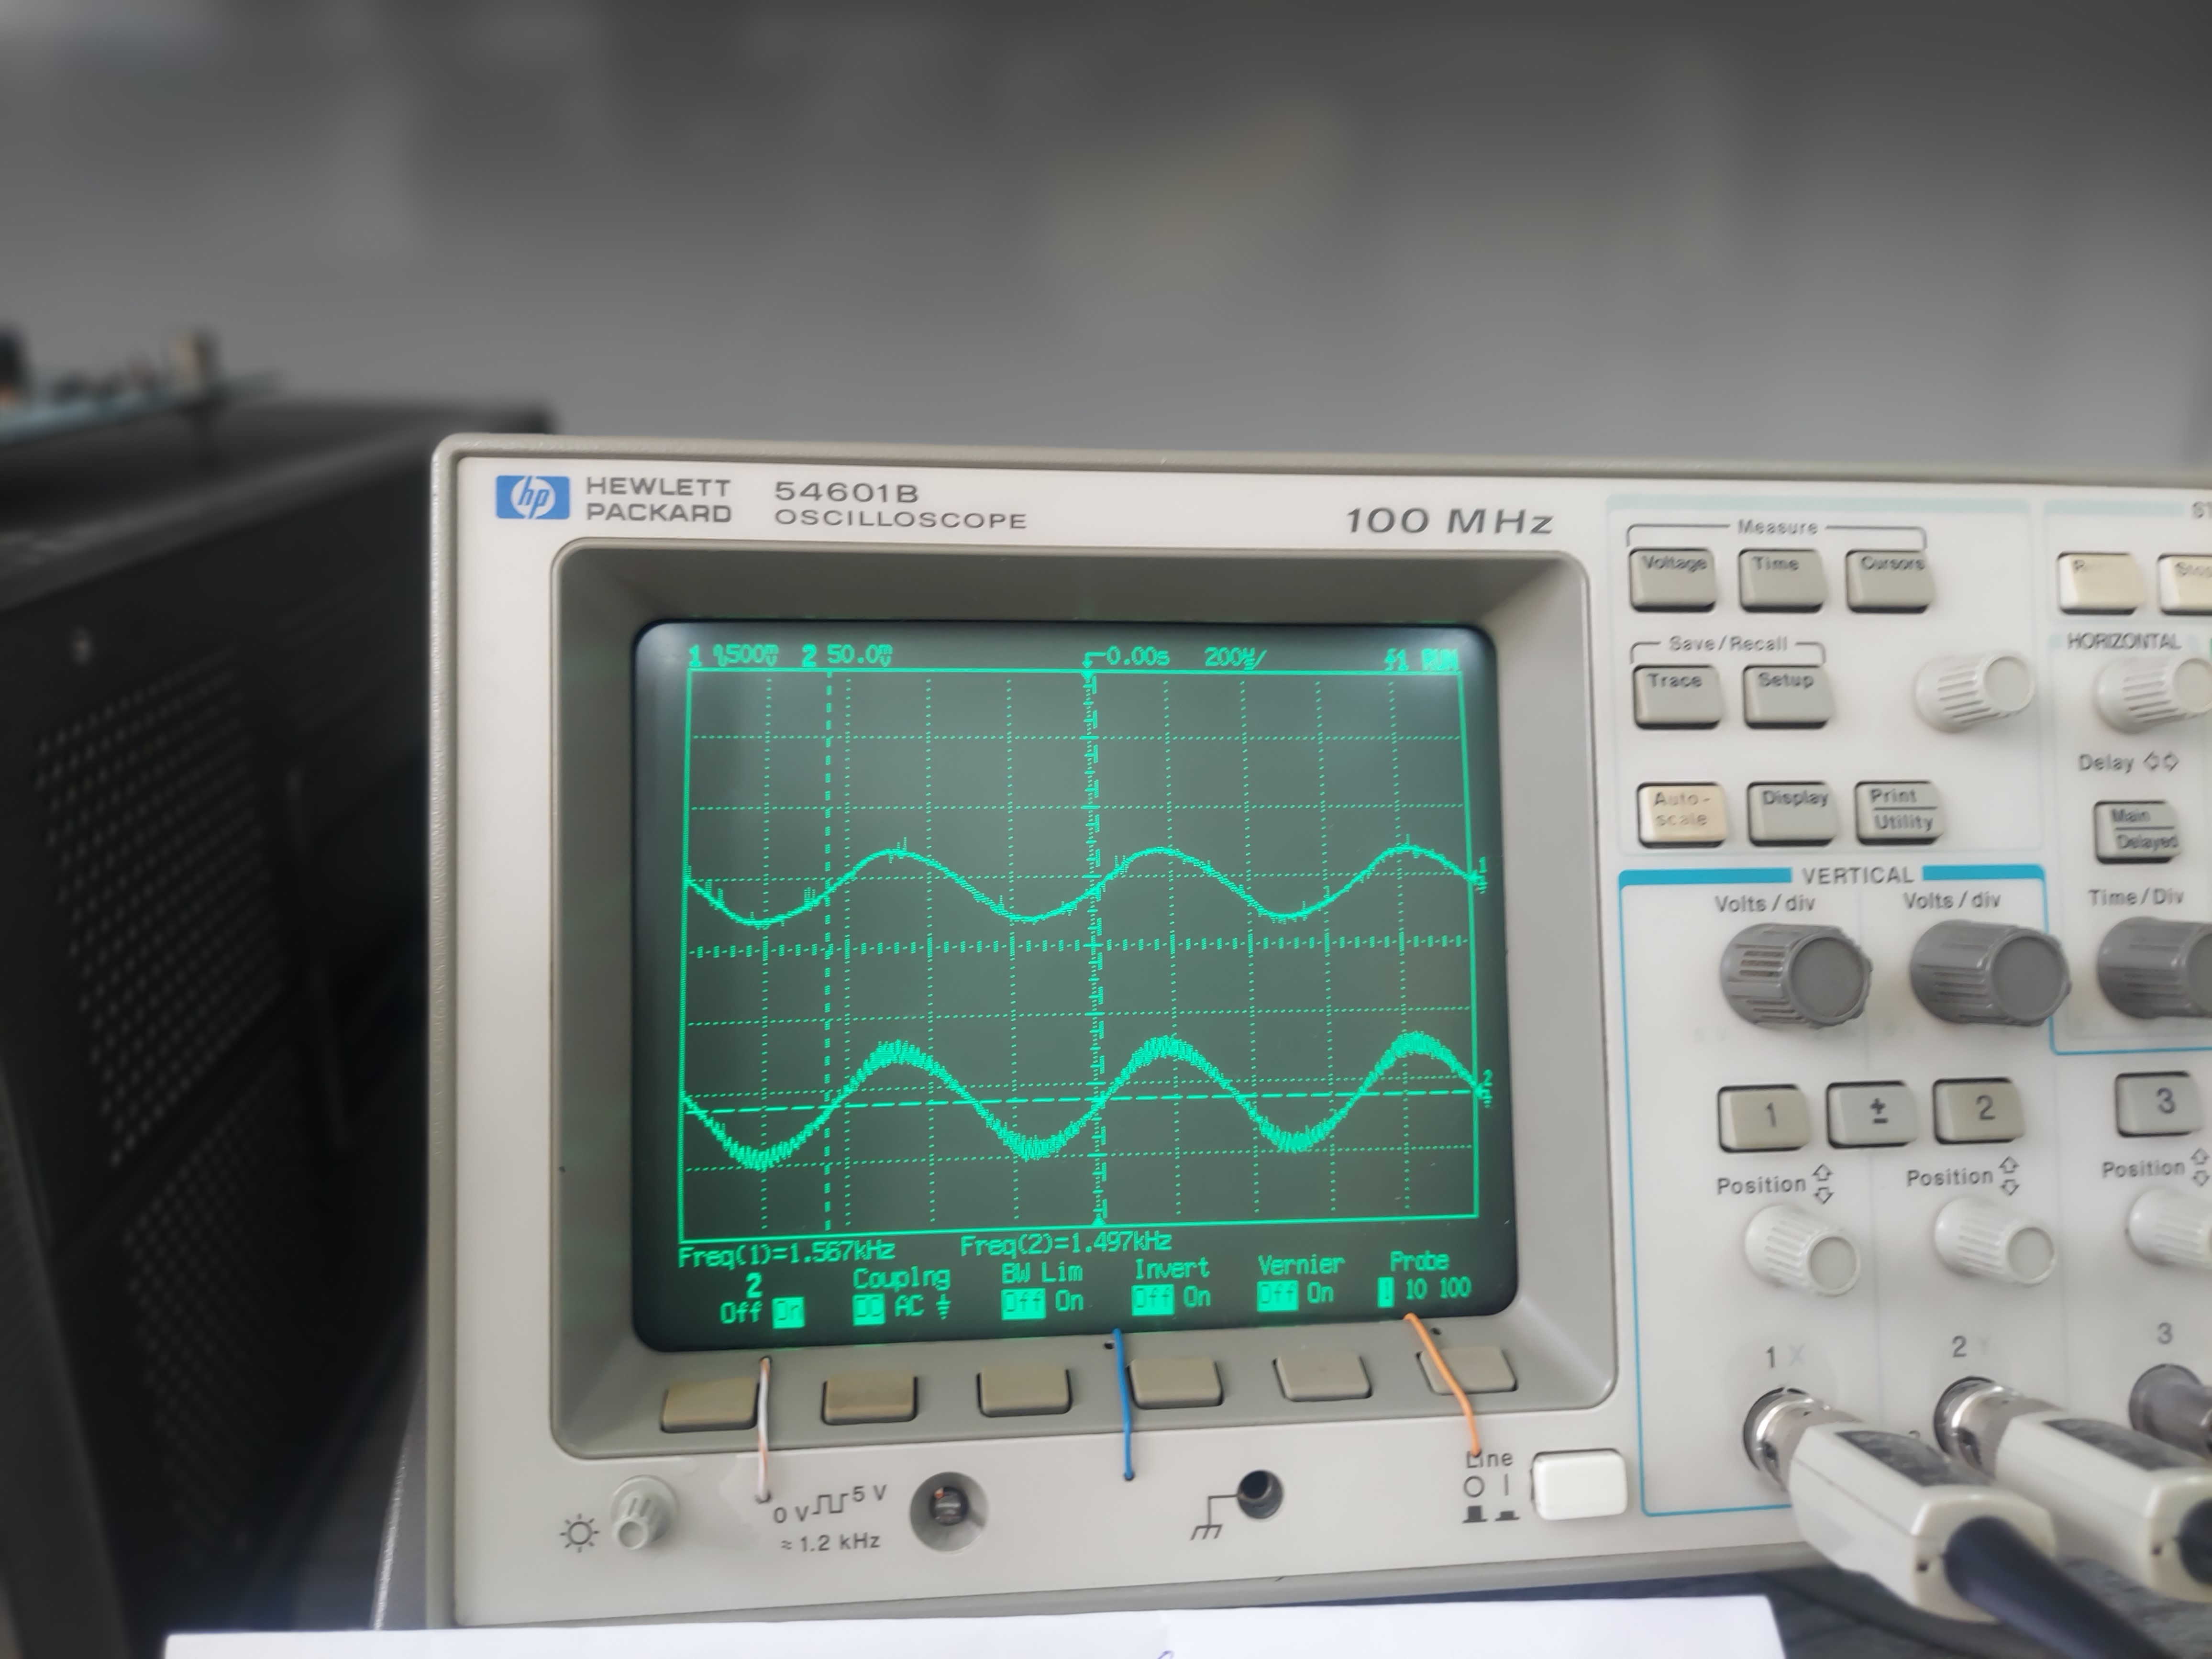
\includegraphics[width=\textwidth]{Imagenes/8-senoidal.jpg}
        \caption{Señal senoidal recuperada}
    \end{subfigure}
    \\[2ex]
    \begin{subfigure}[b]{0.45\textwidth}
        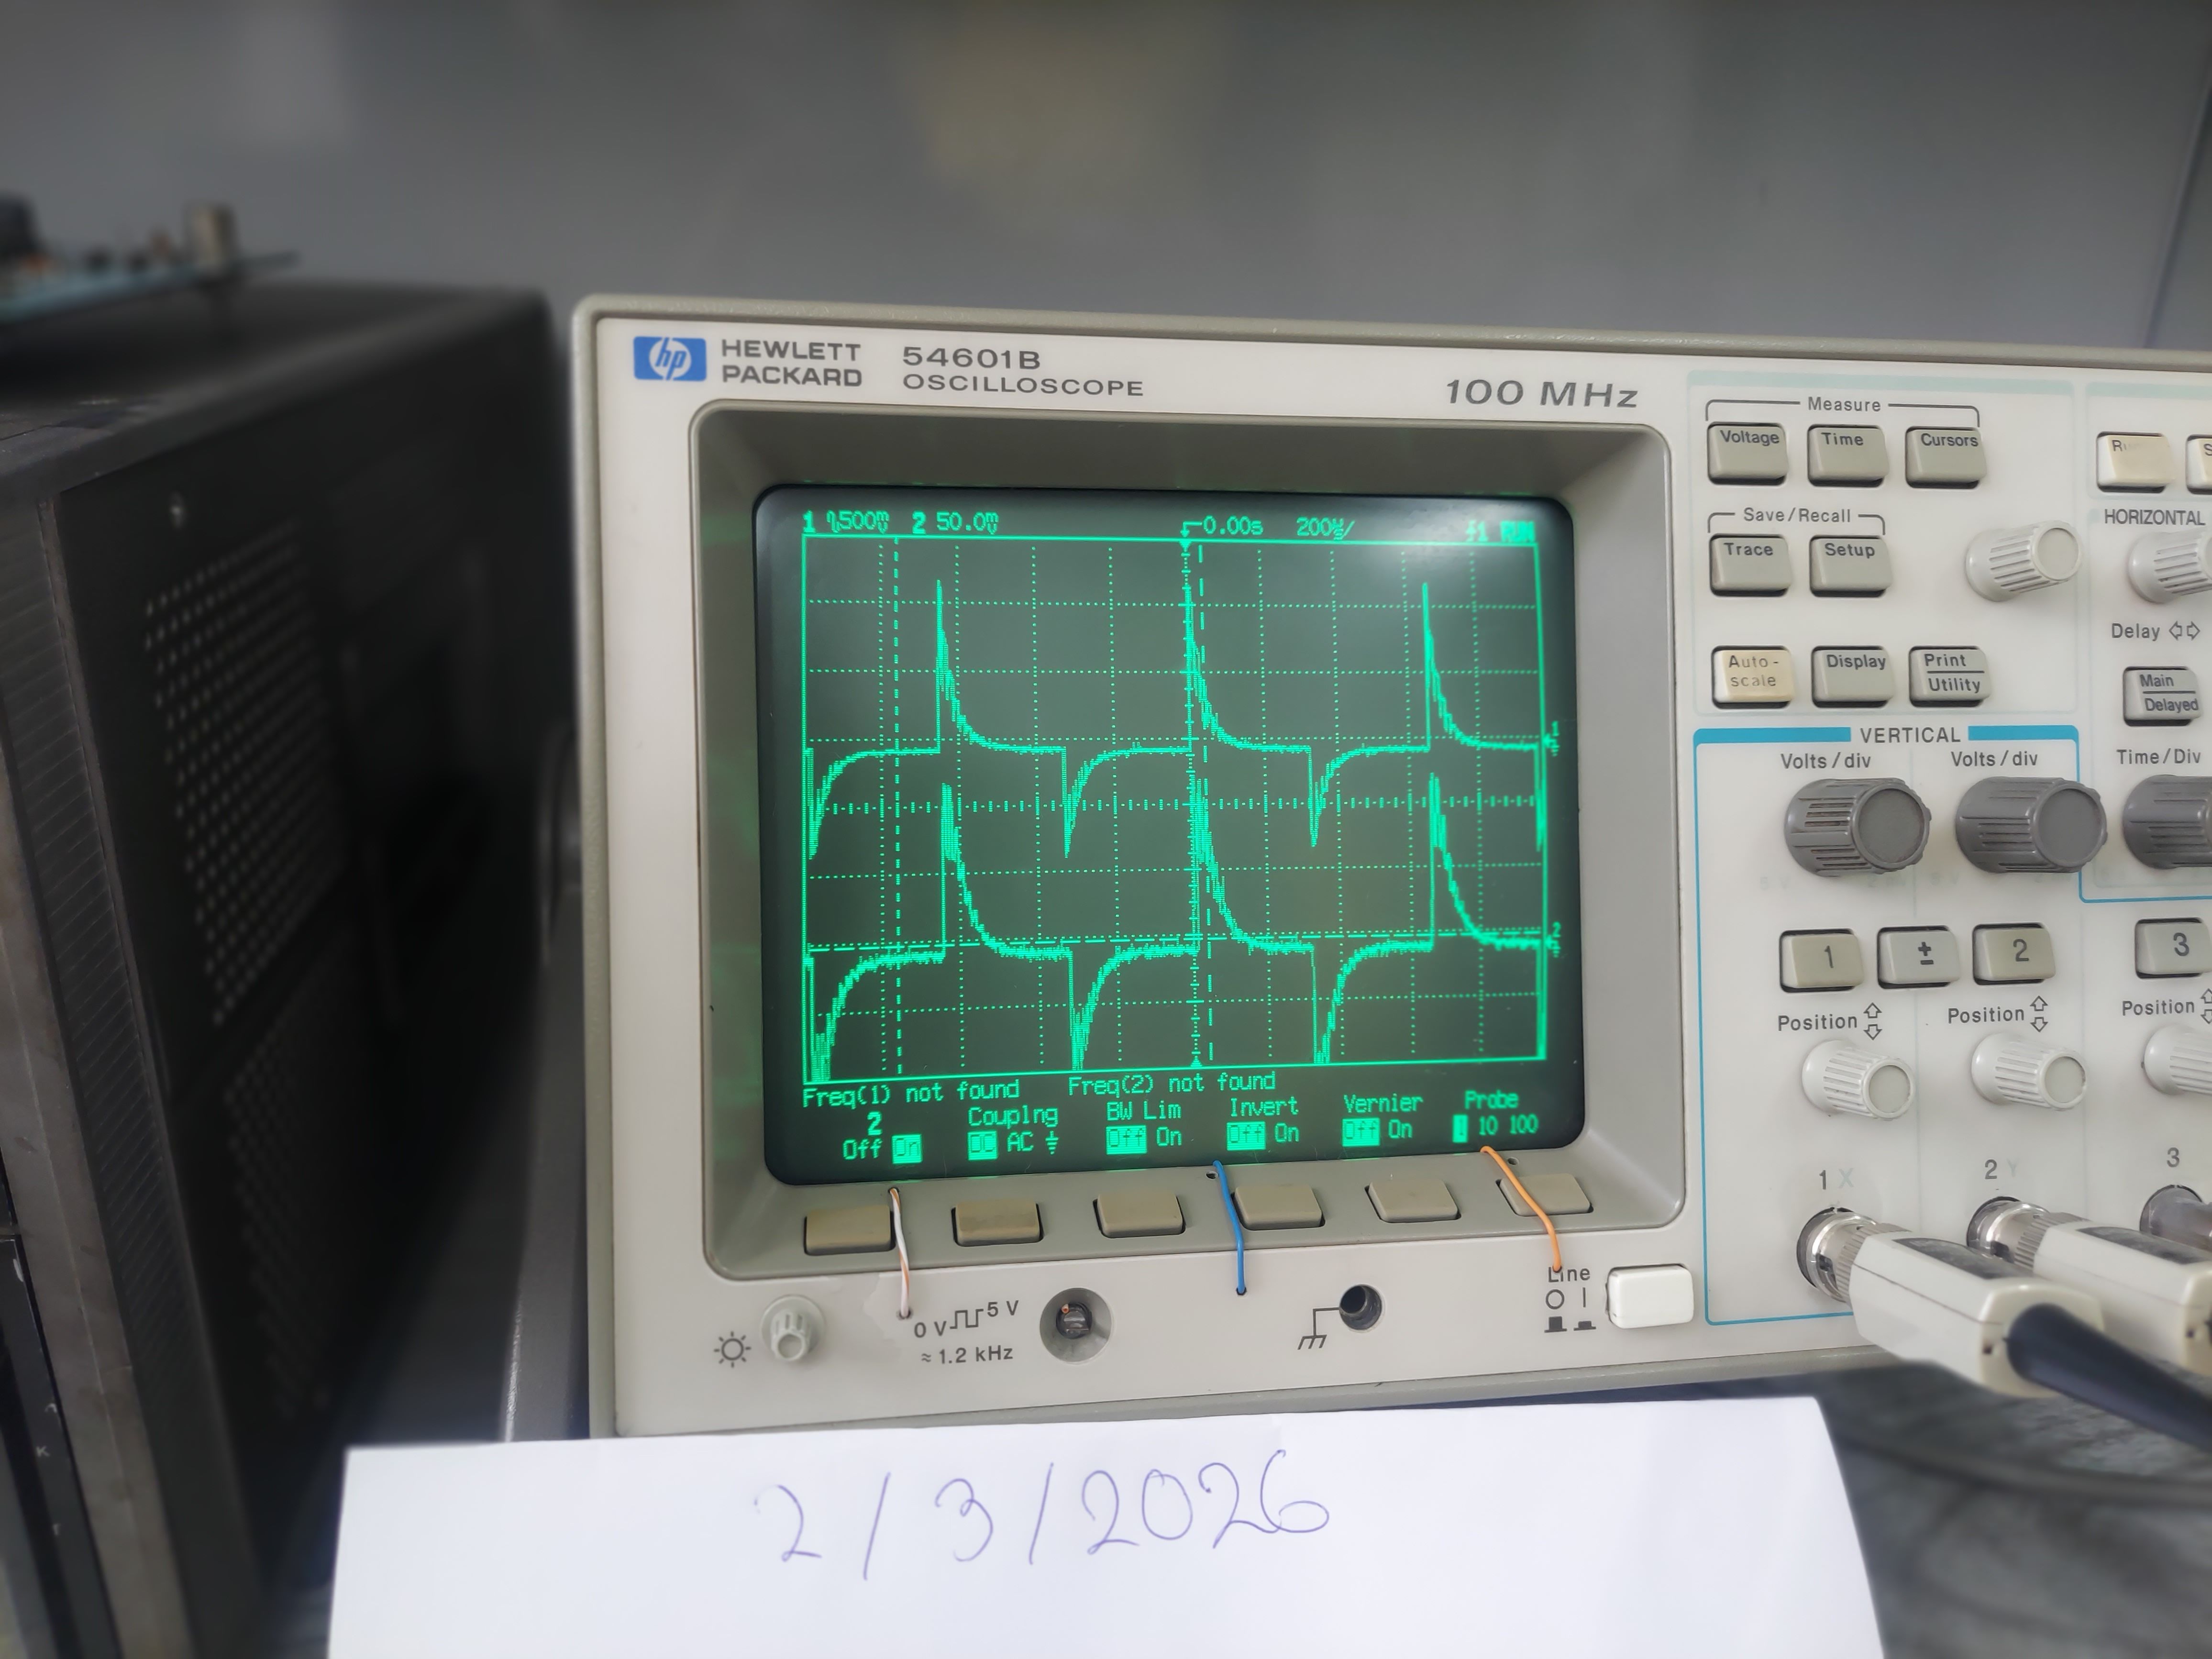
\includegraphics[width=\textwidth]{Imagenes/8-impulso.jpg}
        \caption{Señal de impulso}
    \end{subfigure}
    \hfill
    \begin{subfigure}[b]{0.45\textwidth}
        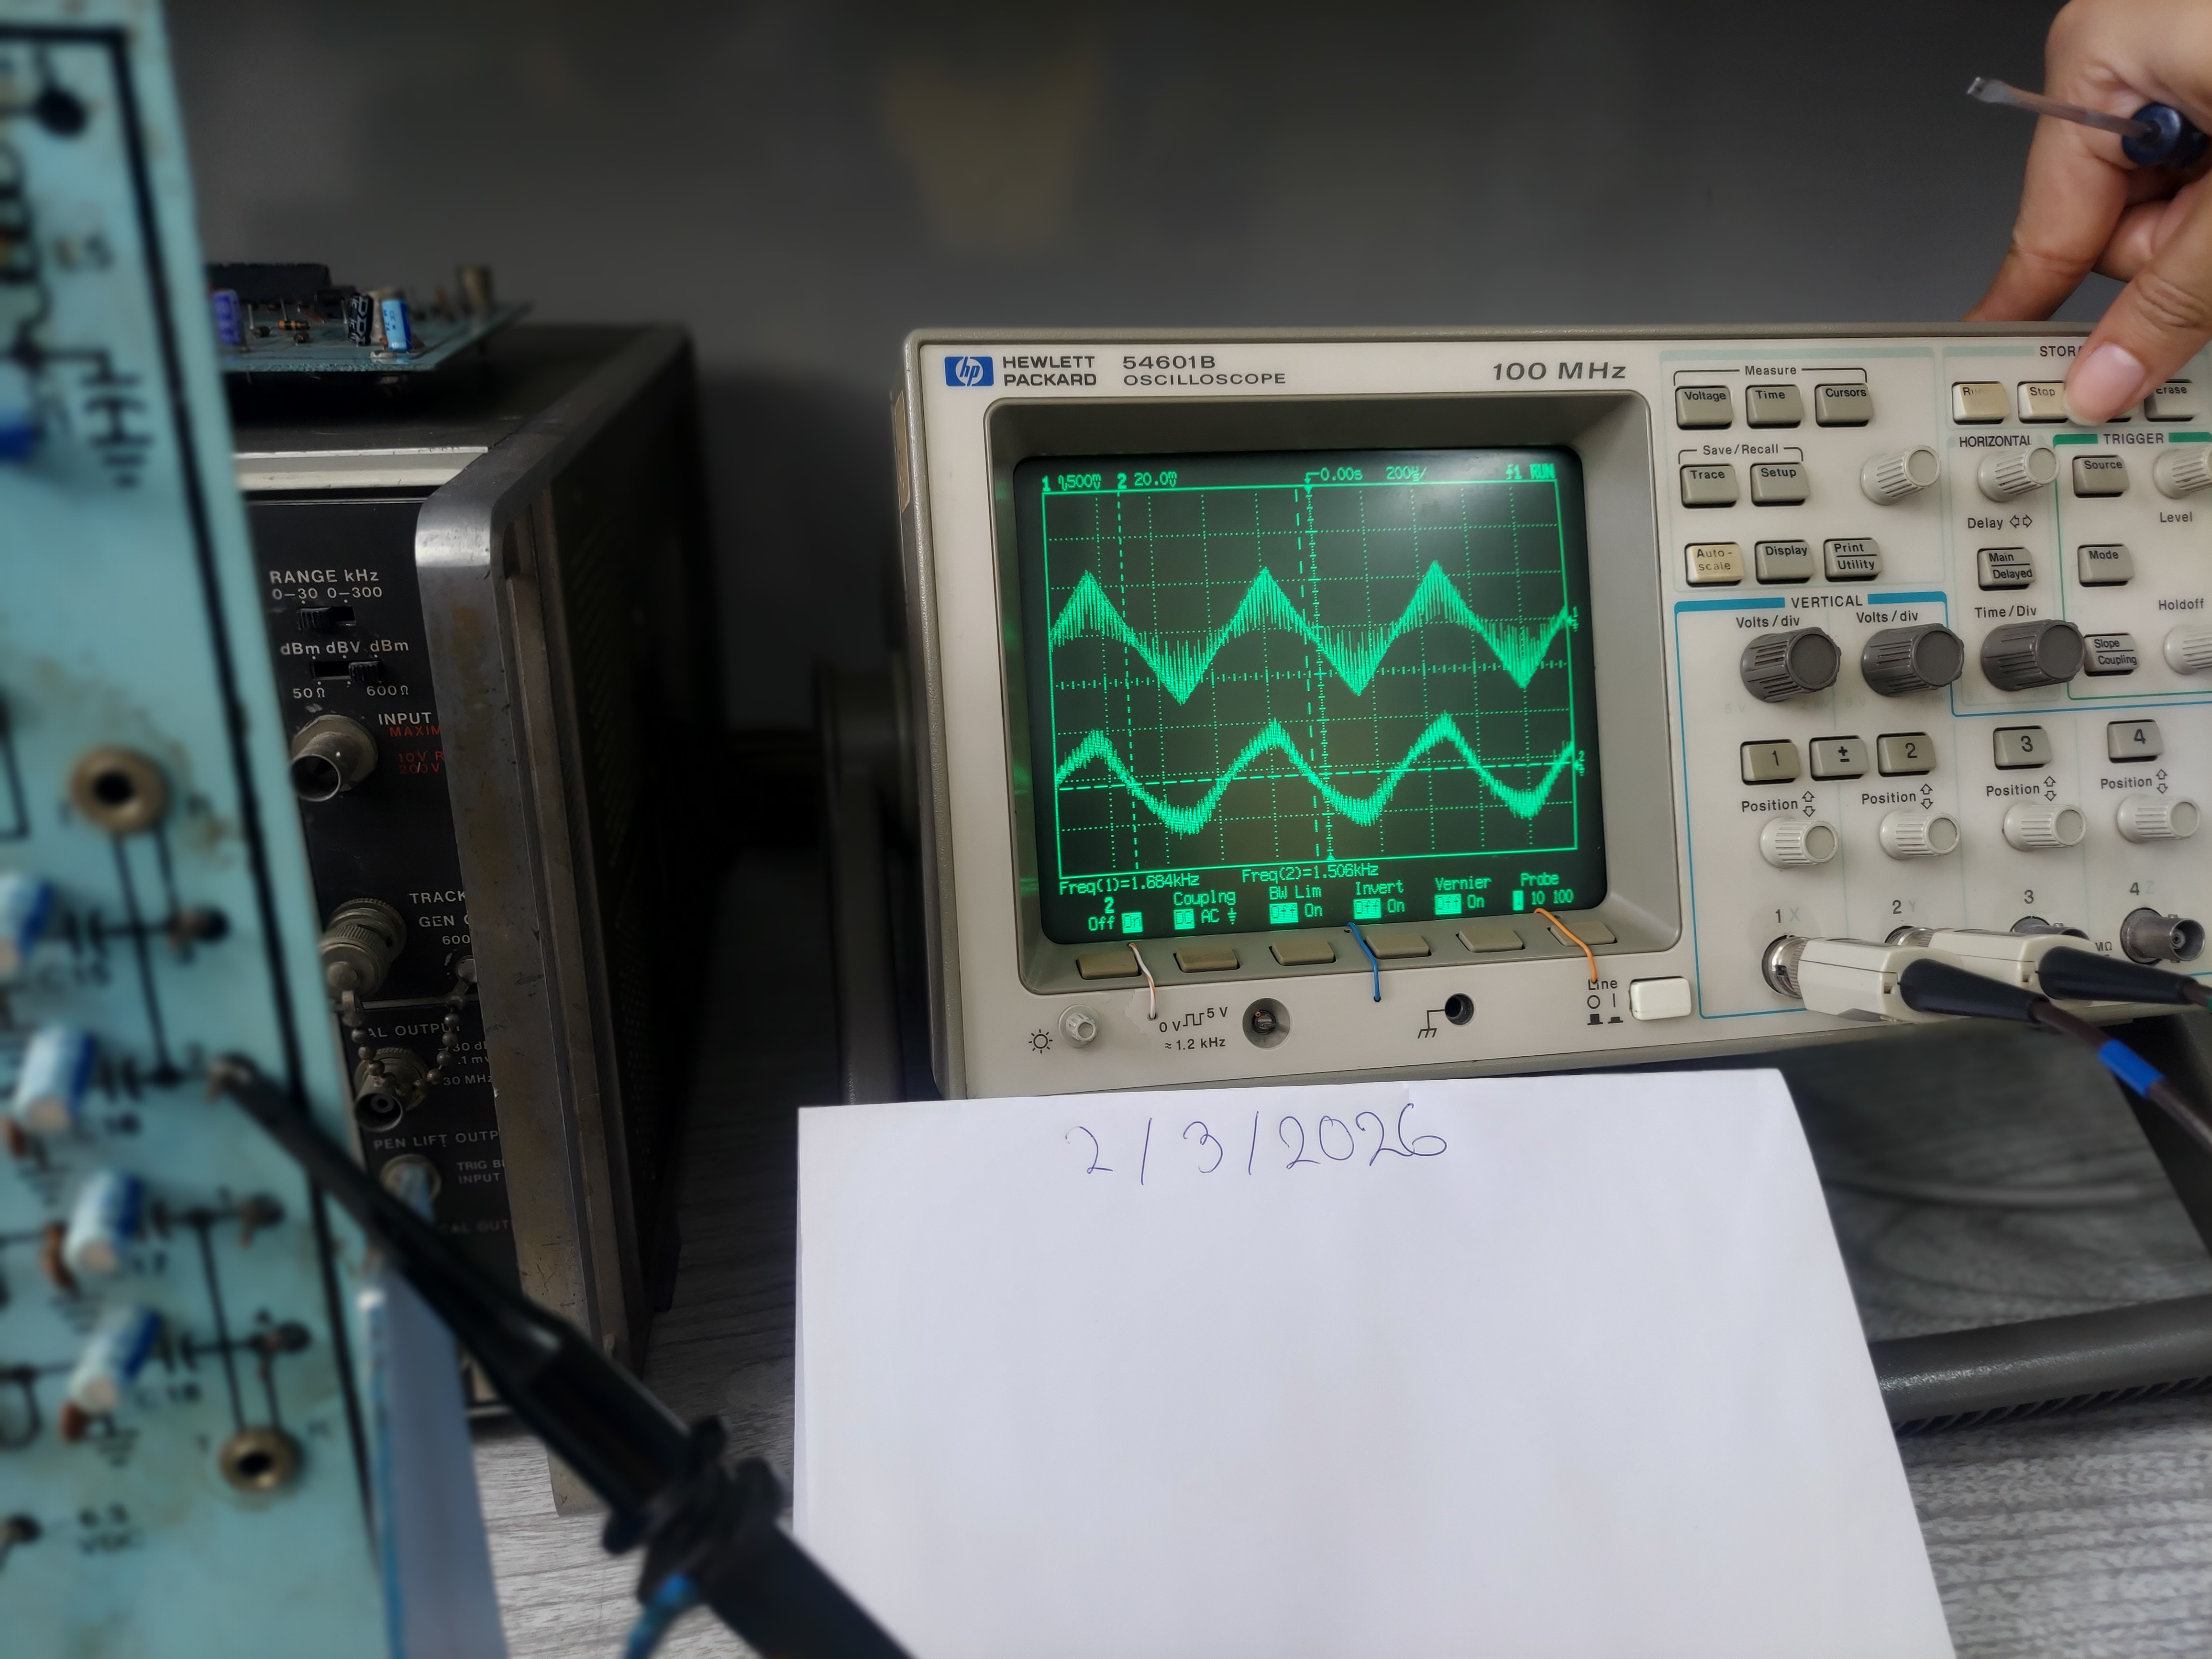
\includegraphics[width=\textwidth]{Imagenes/8-triangular.jpg}
        \caption{Señal triangular recuperada}
    \end{subfigure}
    \caption{Recuperación de reloj y sincronismo con diferentes formas de onda ajustadas.}
\end{figure}

\subsection{Paso 9: Transmisión por Fibra Óptica}
\textbf{Instrucciones:}
\begin{itemize}
    \item Desconecte el cable coaxial que une los módulos de transmisión y recepción, y una conecte una fibra óptica entre los conectores apropiados. Pase el conmutador a la posición OPTO. Compare las señales en TP2 y TP9. La señal en TP2 controla la corriente de alimentación del diodo emisor de luz D2.
    \item Transfiera la punta de prueba de TP2 a TP11 para observar la señal recibida. La señal de luz actúa sobre el fotodiodo D1 para recuperar la señal de la banda base.
    \item Varíe el control GAIN ADJ y observe los efectos sobre la señal recibida. Investigue sobre el funcionamiento de los circuitos modulador y demodulador de luz utilizados en la práctica.
\end{itemize}

\begin{figure}[H]
    \centering
    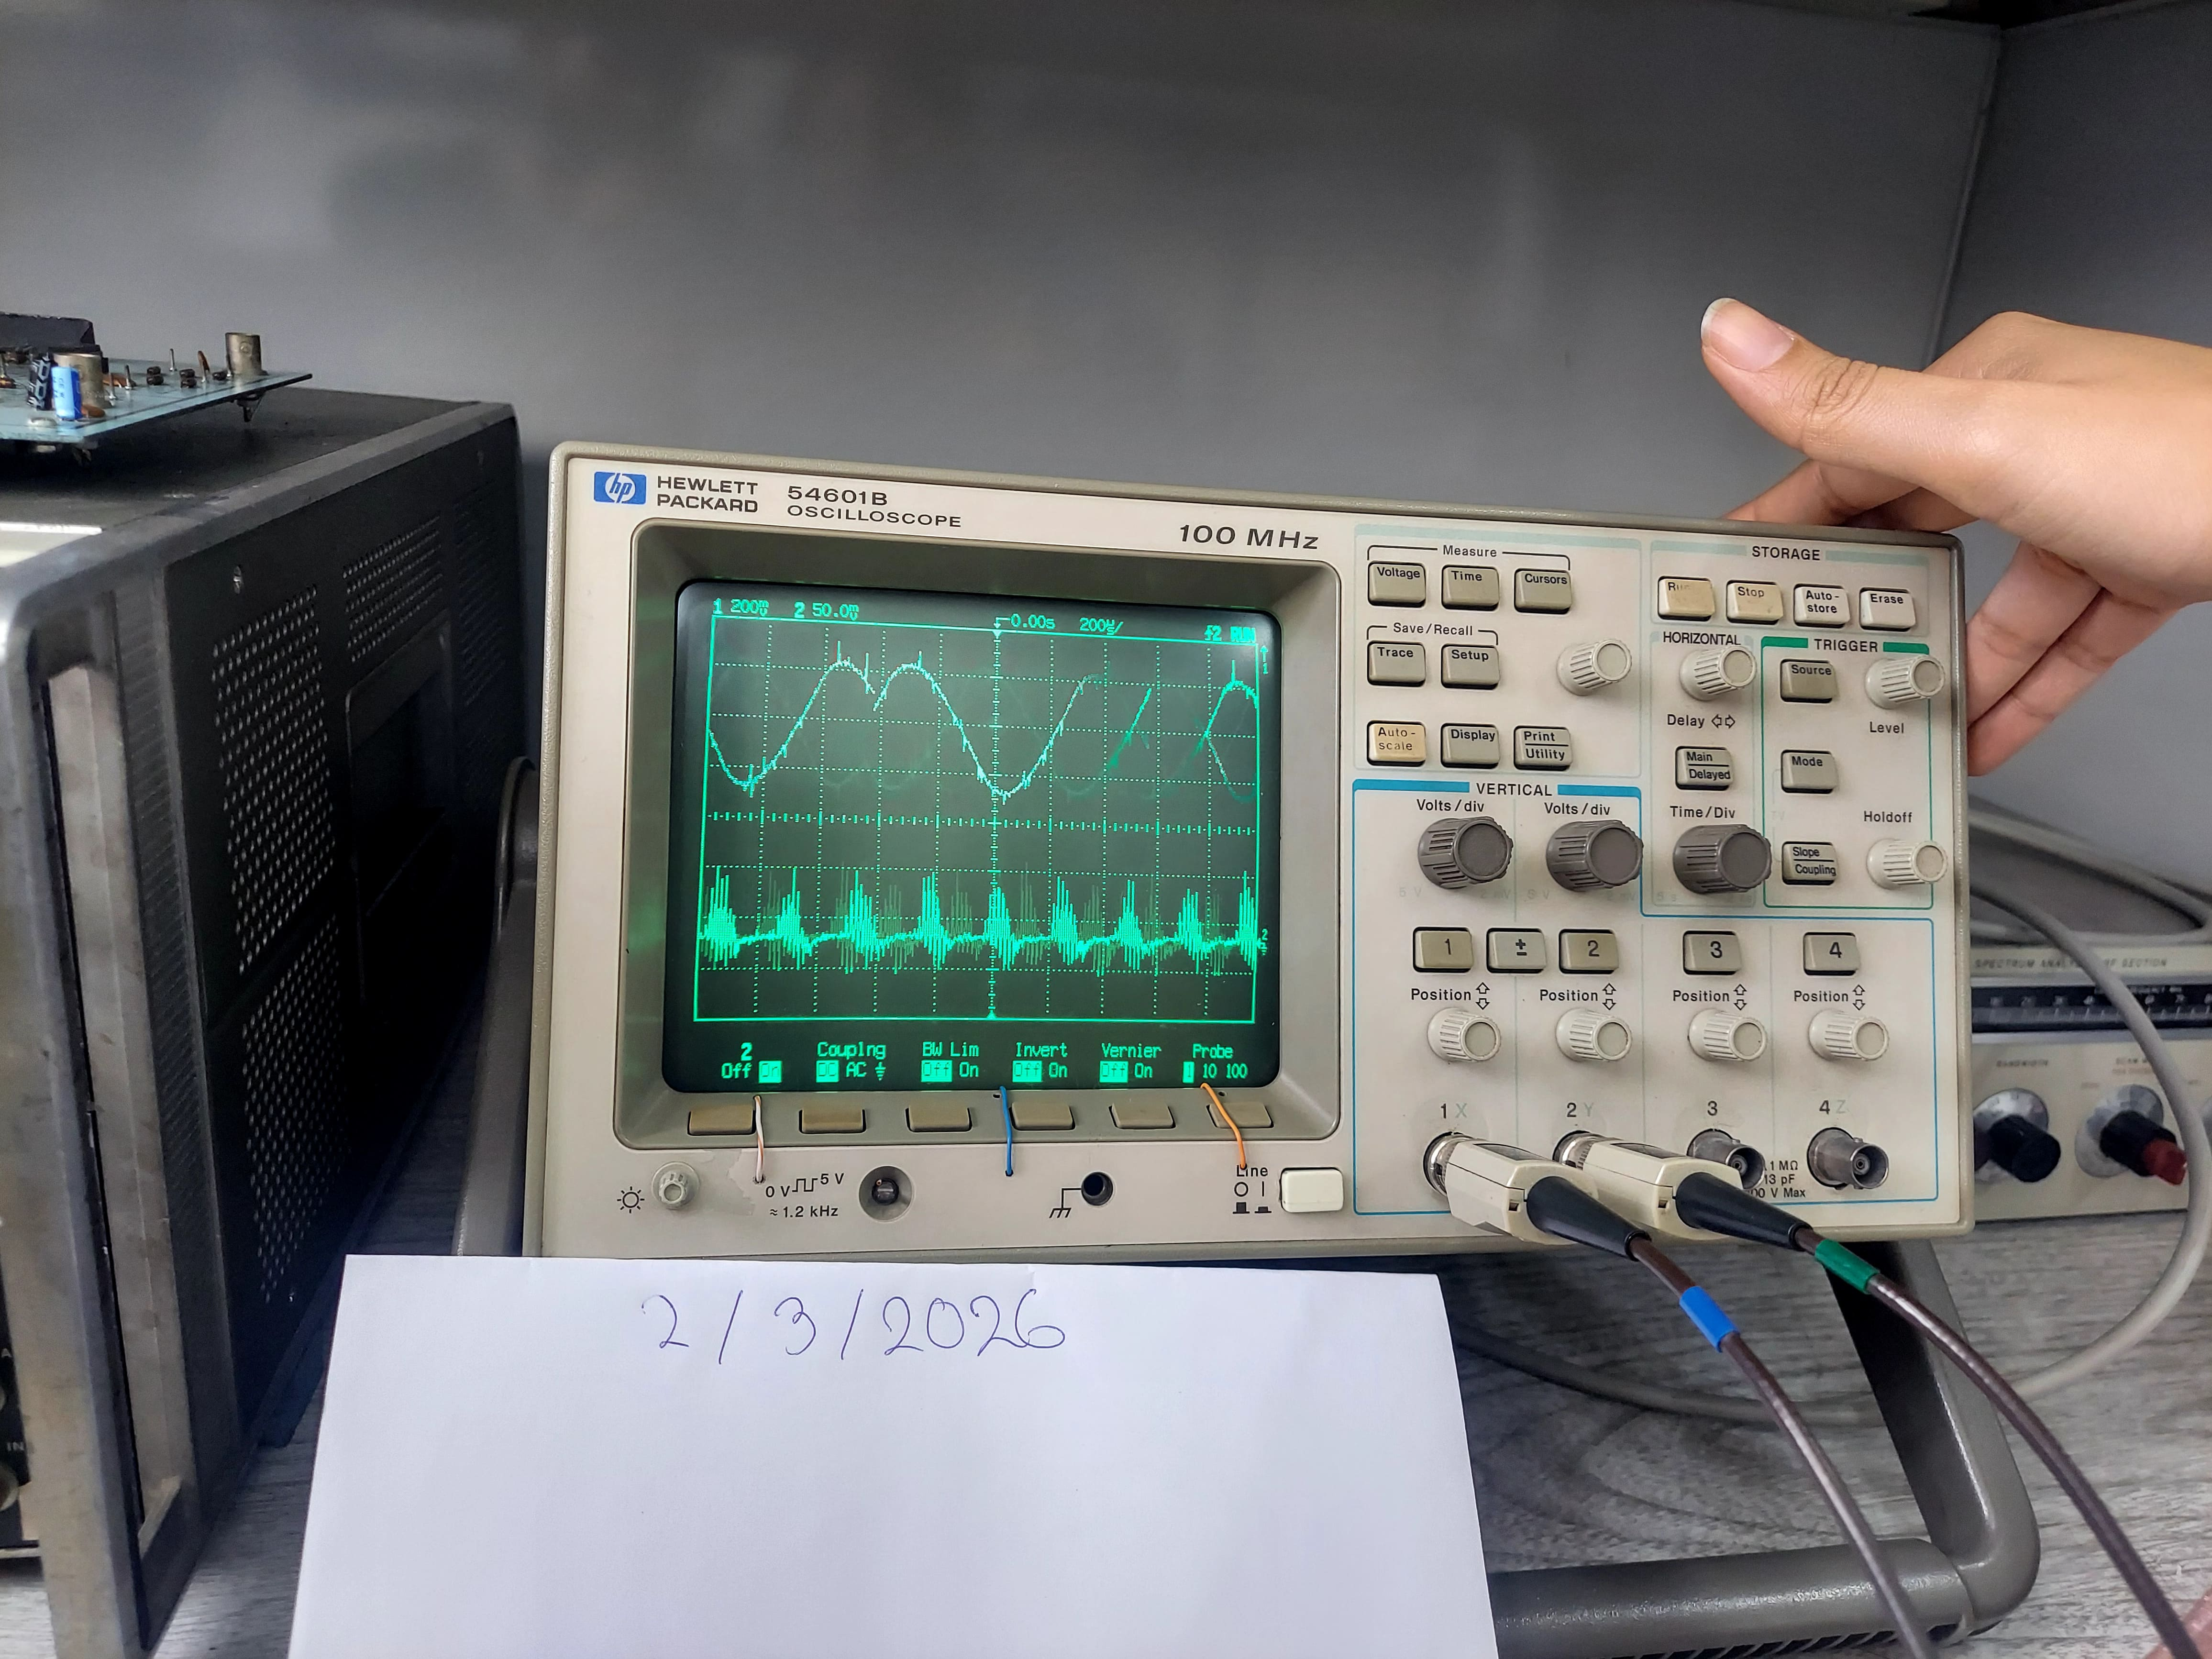
\includegraphics[width=0.8\textwidth]{Imagenes/9-1.jpg}
    \caption{Conexión por fibra óptica.}
\end{figure}

\begin{figure}[H]
    \centering
    \begin{subfigure}[b]{0.45\textwidth}
        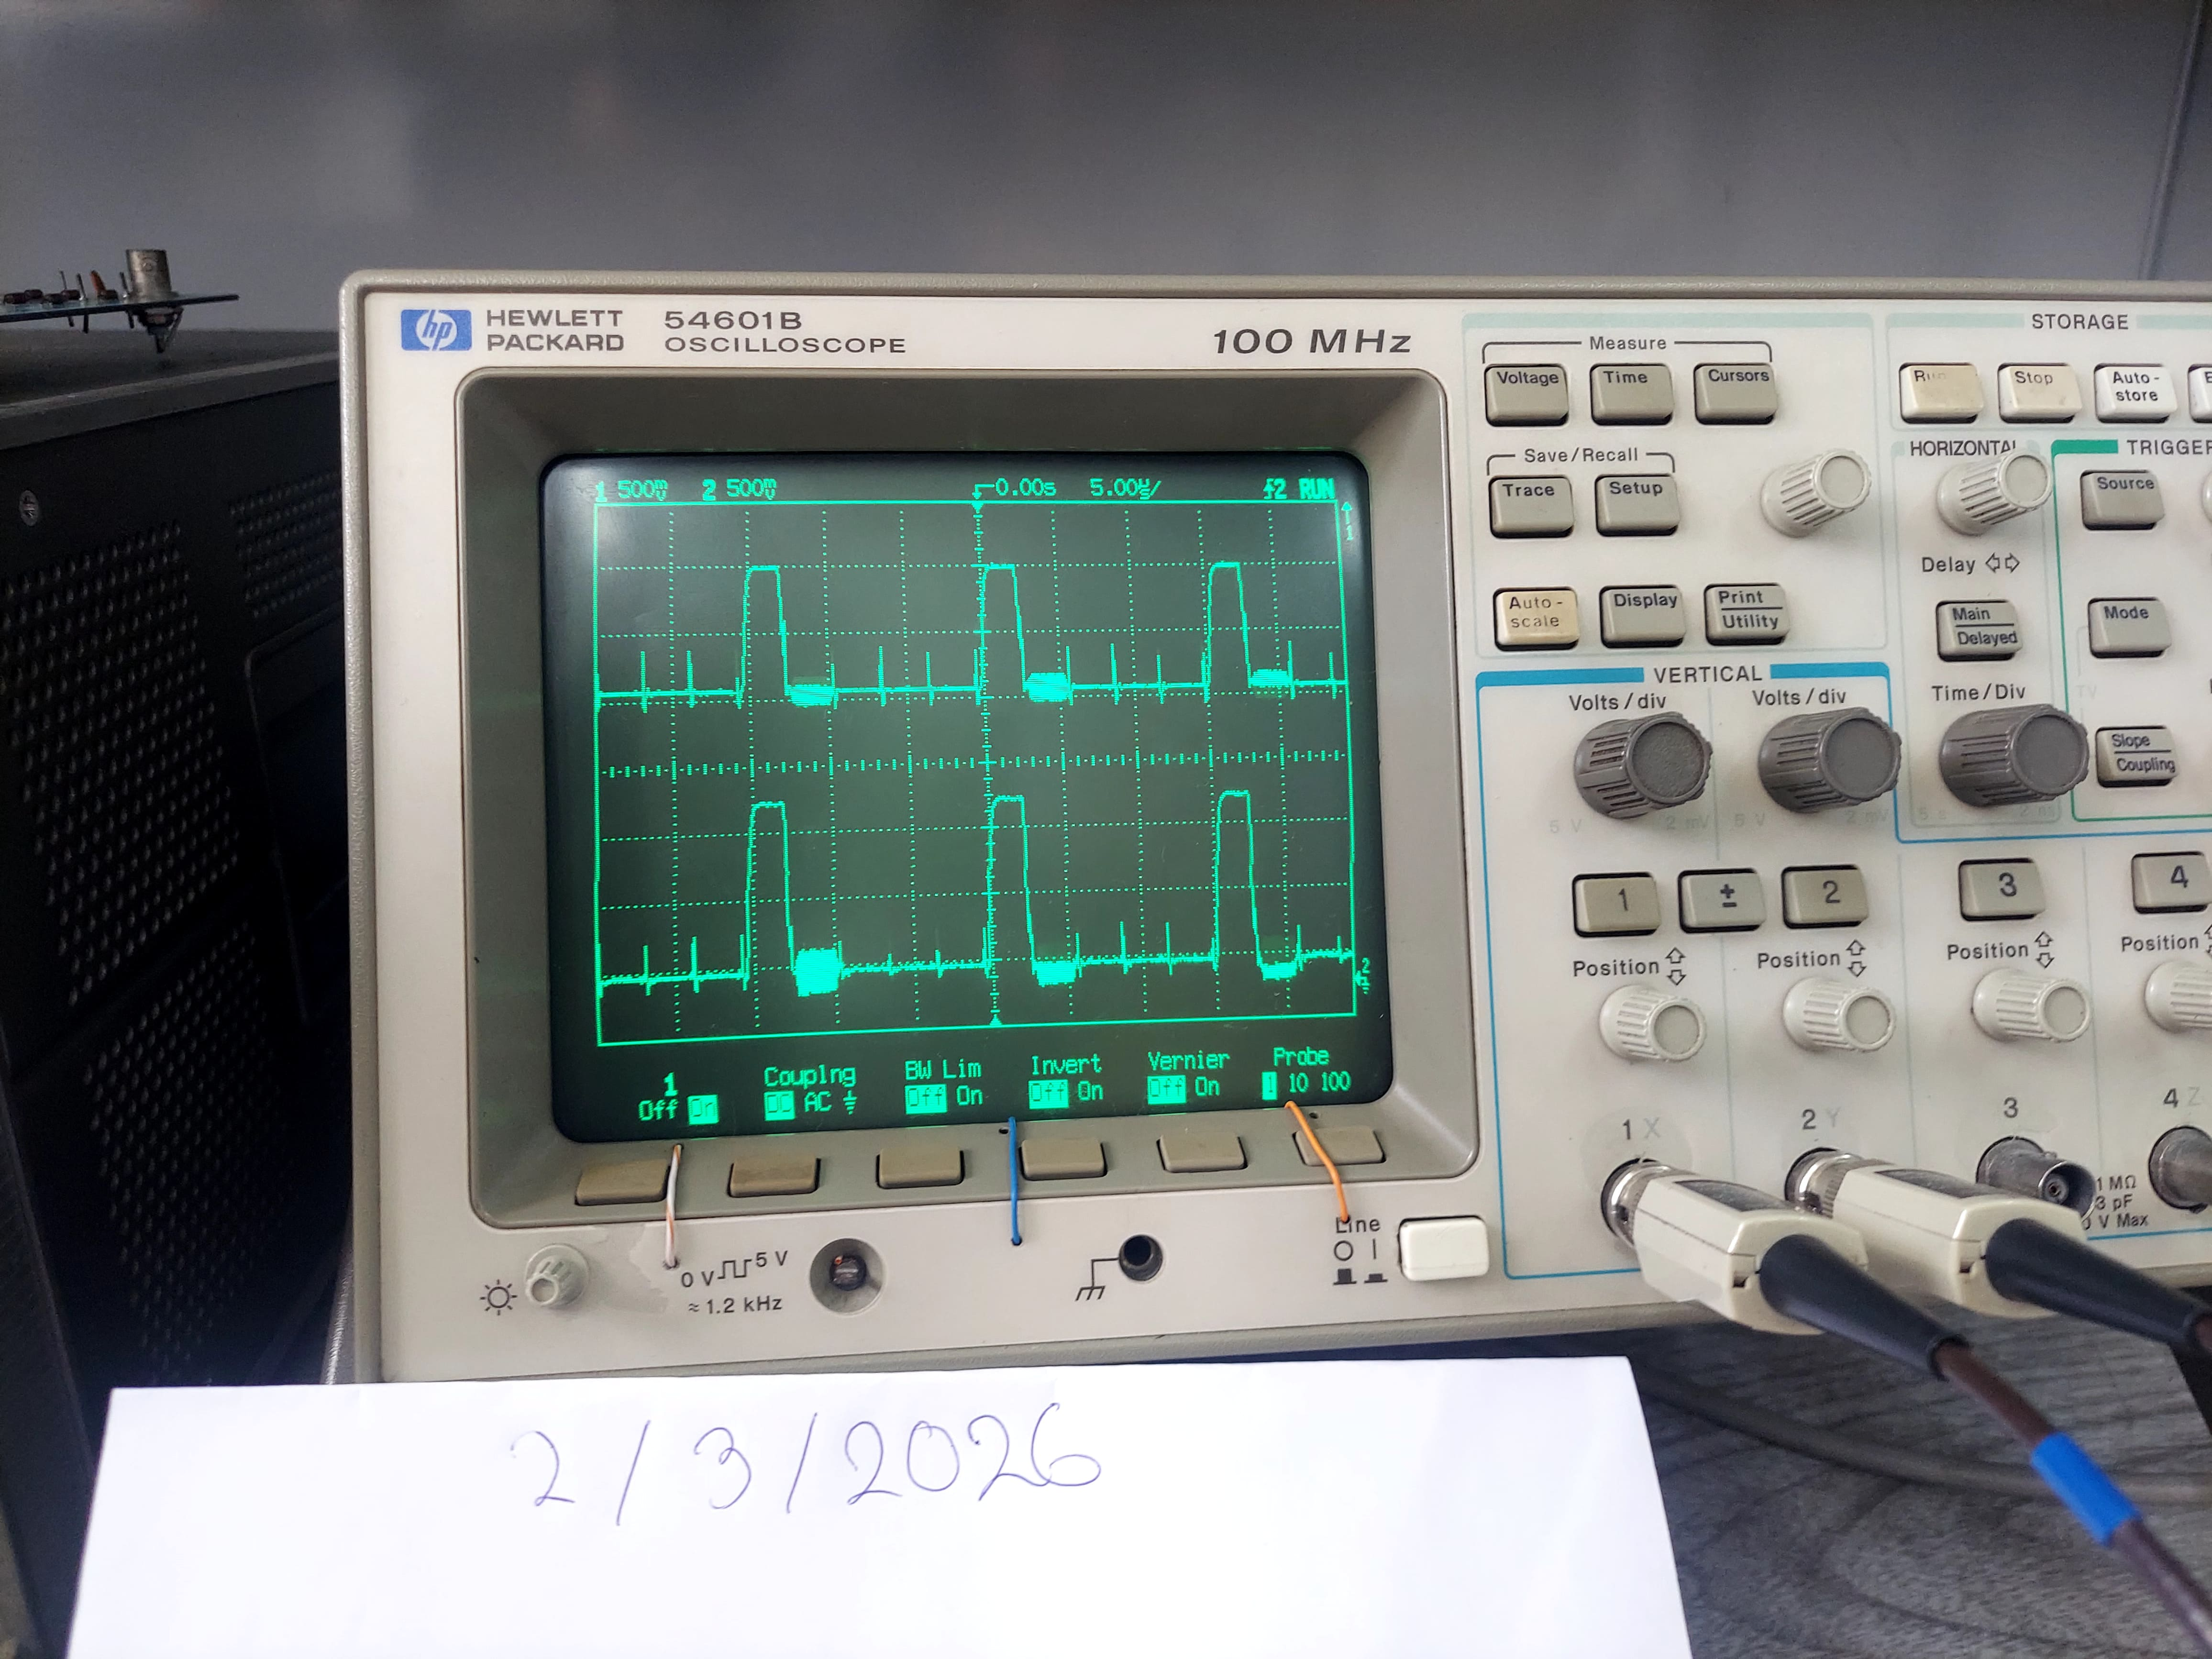
\includegraphics[width=\textwidth]{Imagenes/9-ajuste-gain-1.jpg}
        \caption{Ajuste 1}
    \end{subfigure}
    \hfill
    \begin{subfigure}[b]{0.45\textwidth}
        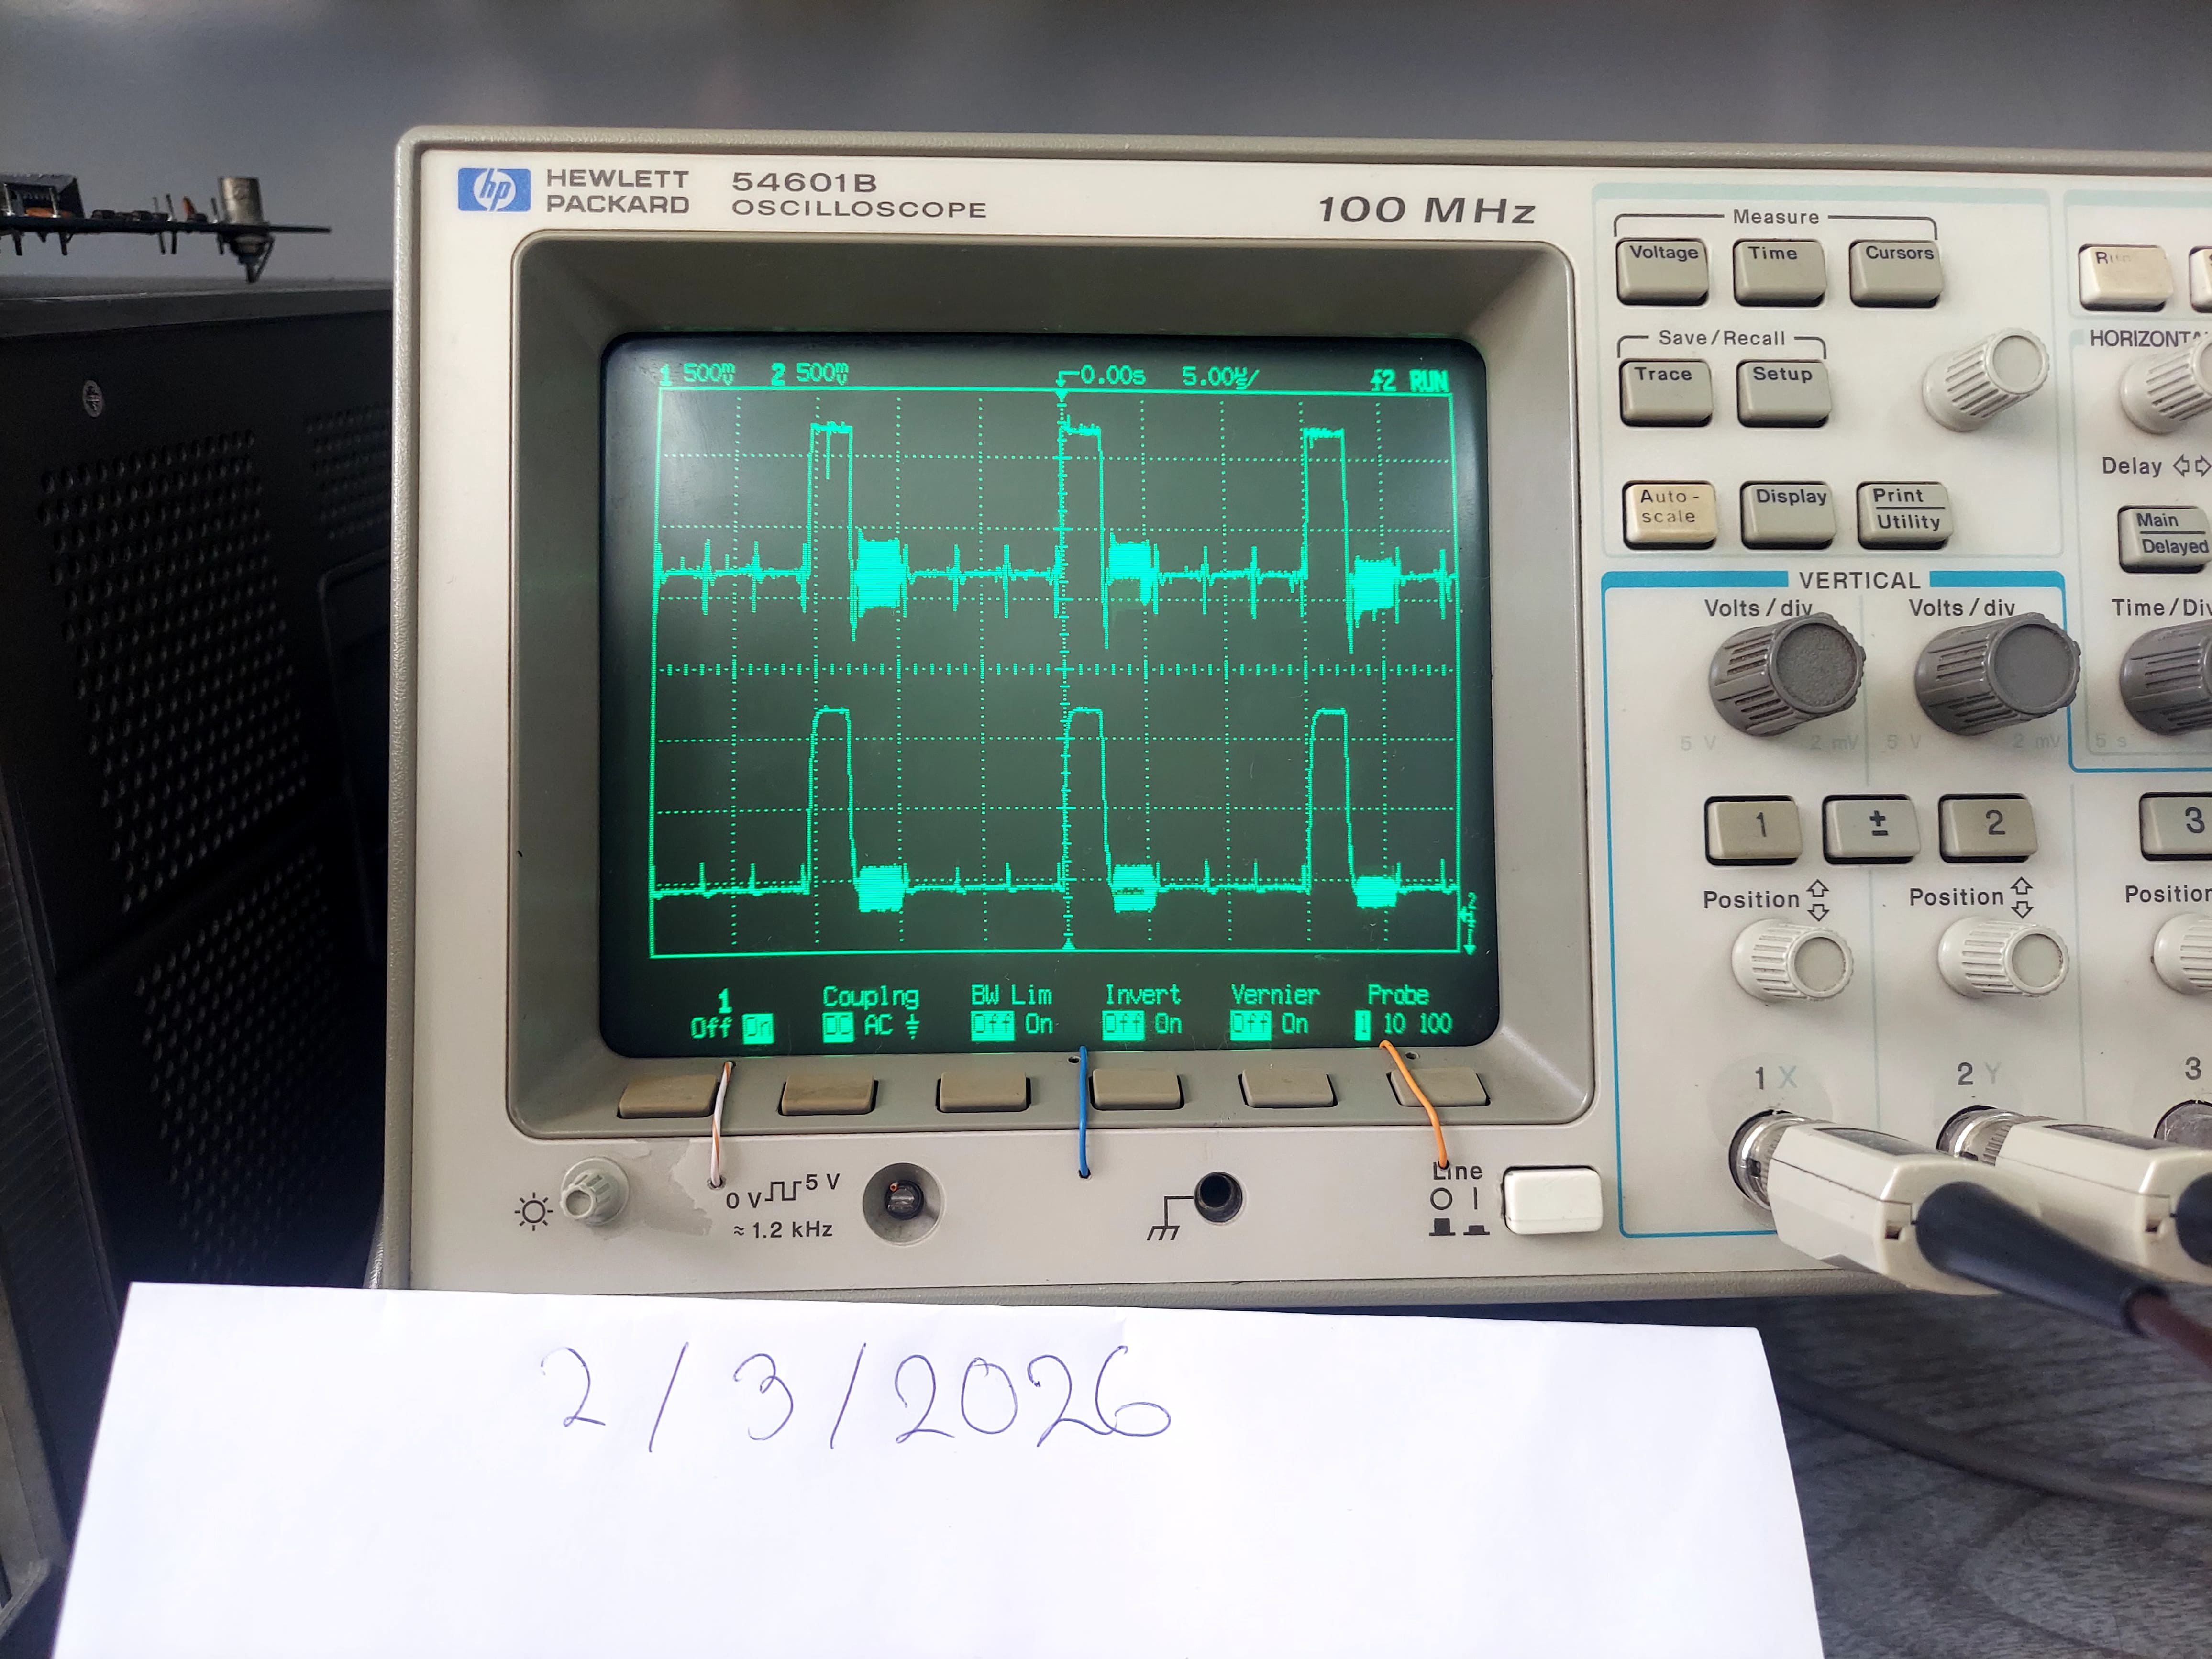
\includegraphics[width=\textwidth]{Imagenes/9-ajuste-gain-2.jpg}
        \caption{Ajuste 2}
    \end{subfigure}
    \\[2ex]
    \begin{subfigure}[b]{0.45\textwidth}
        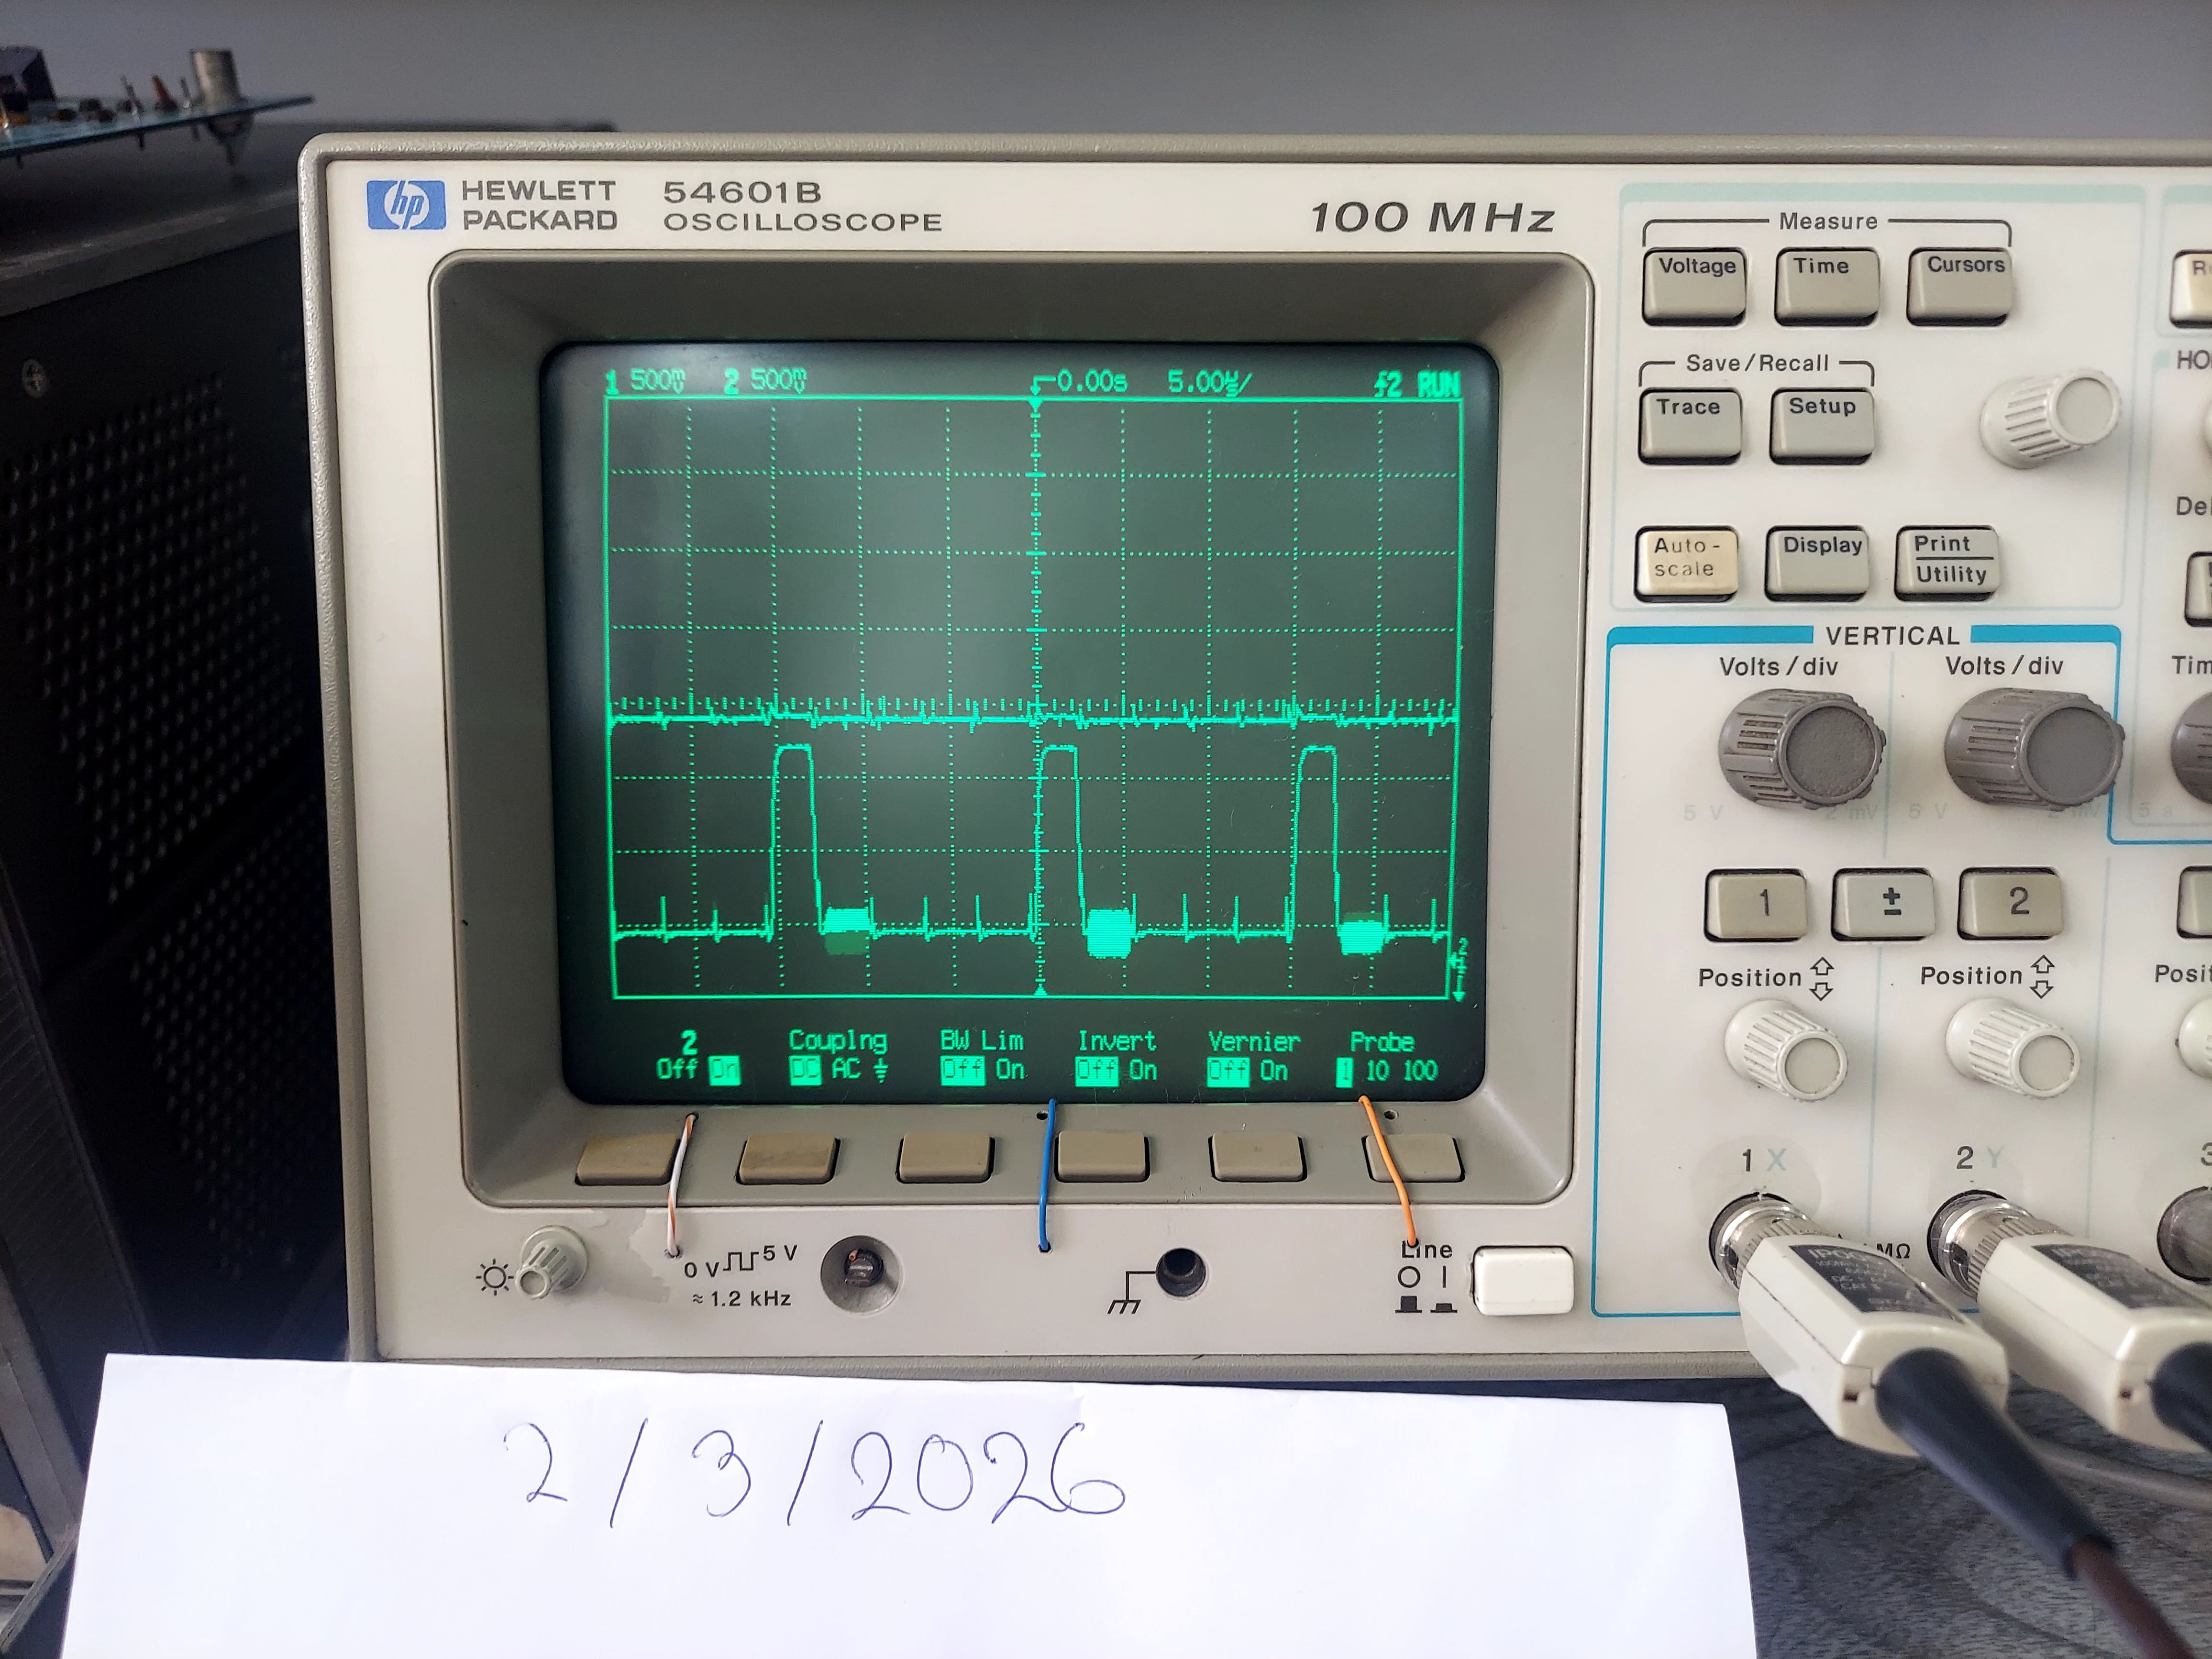
\includegraphics[width=\textwidth]{Imagenes/9-ajuste-gain-3.jpg}
        \caption{Ajuste 3}
    \end{subfigure}
    \hfill
    \begin{subfigure}[b]{0.45\textwidth}
        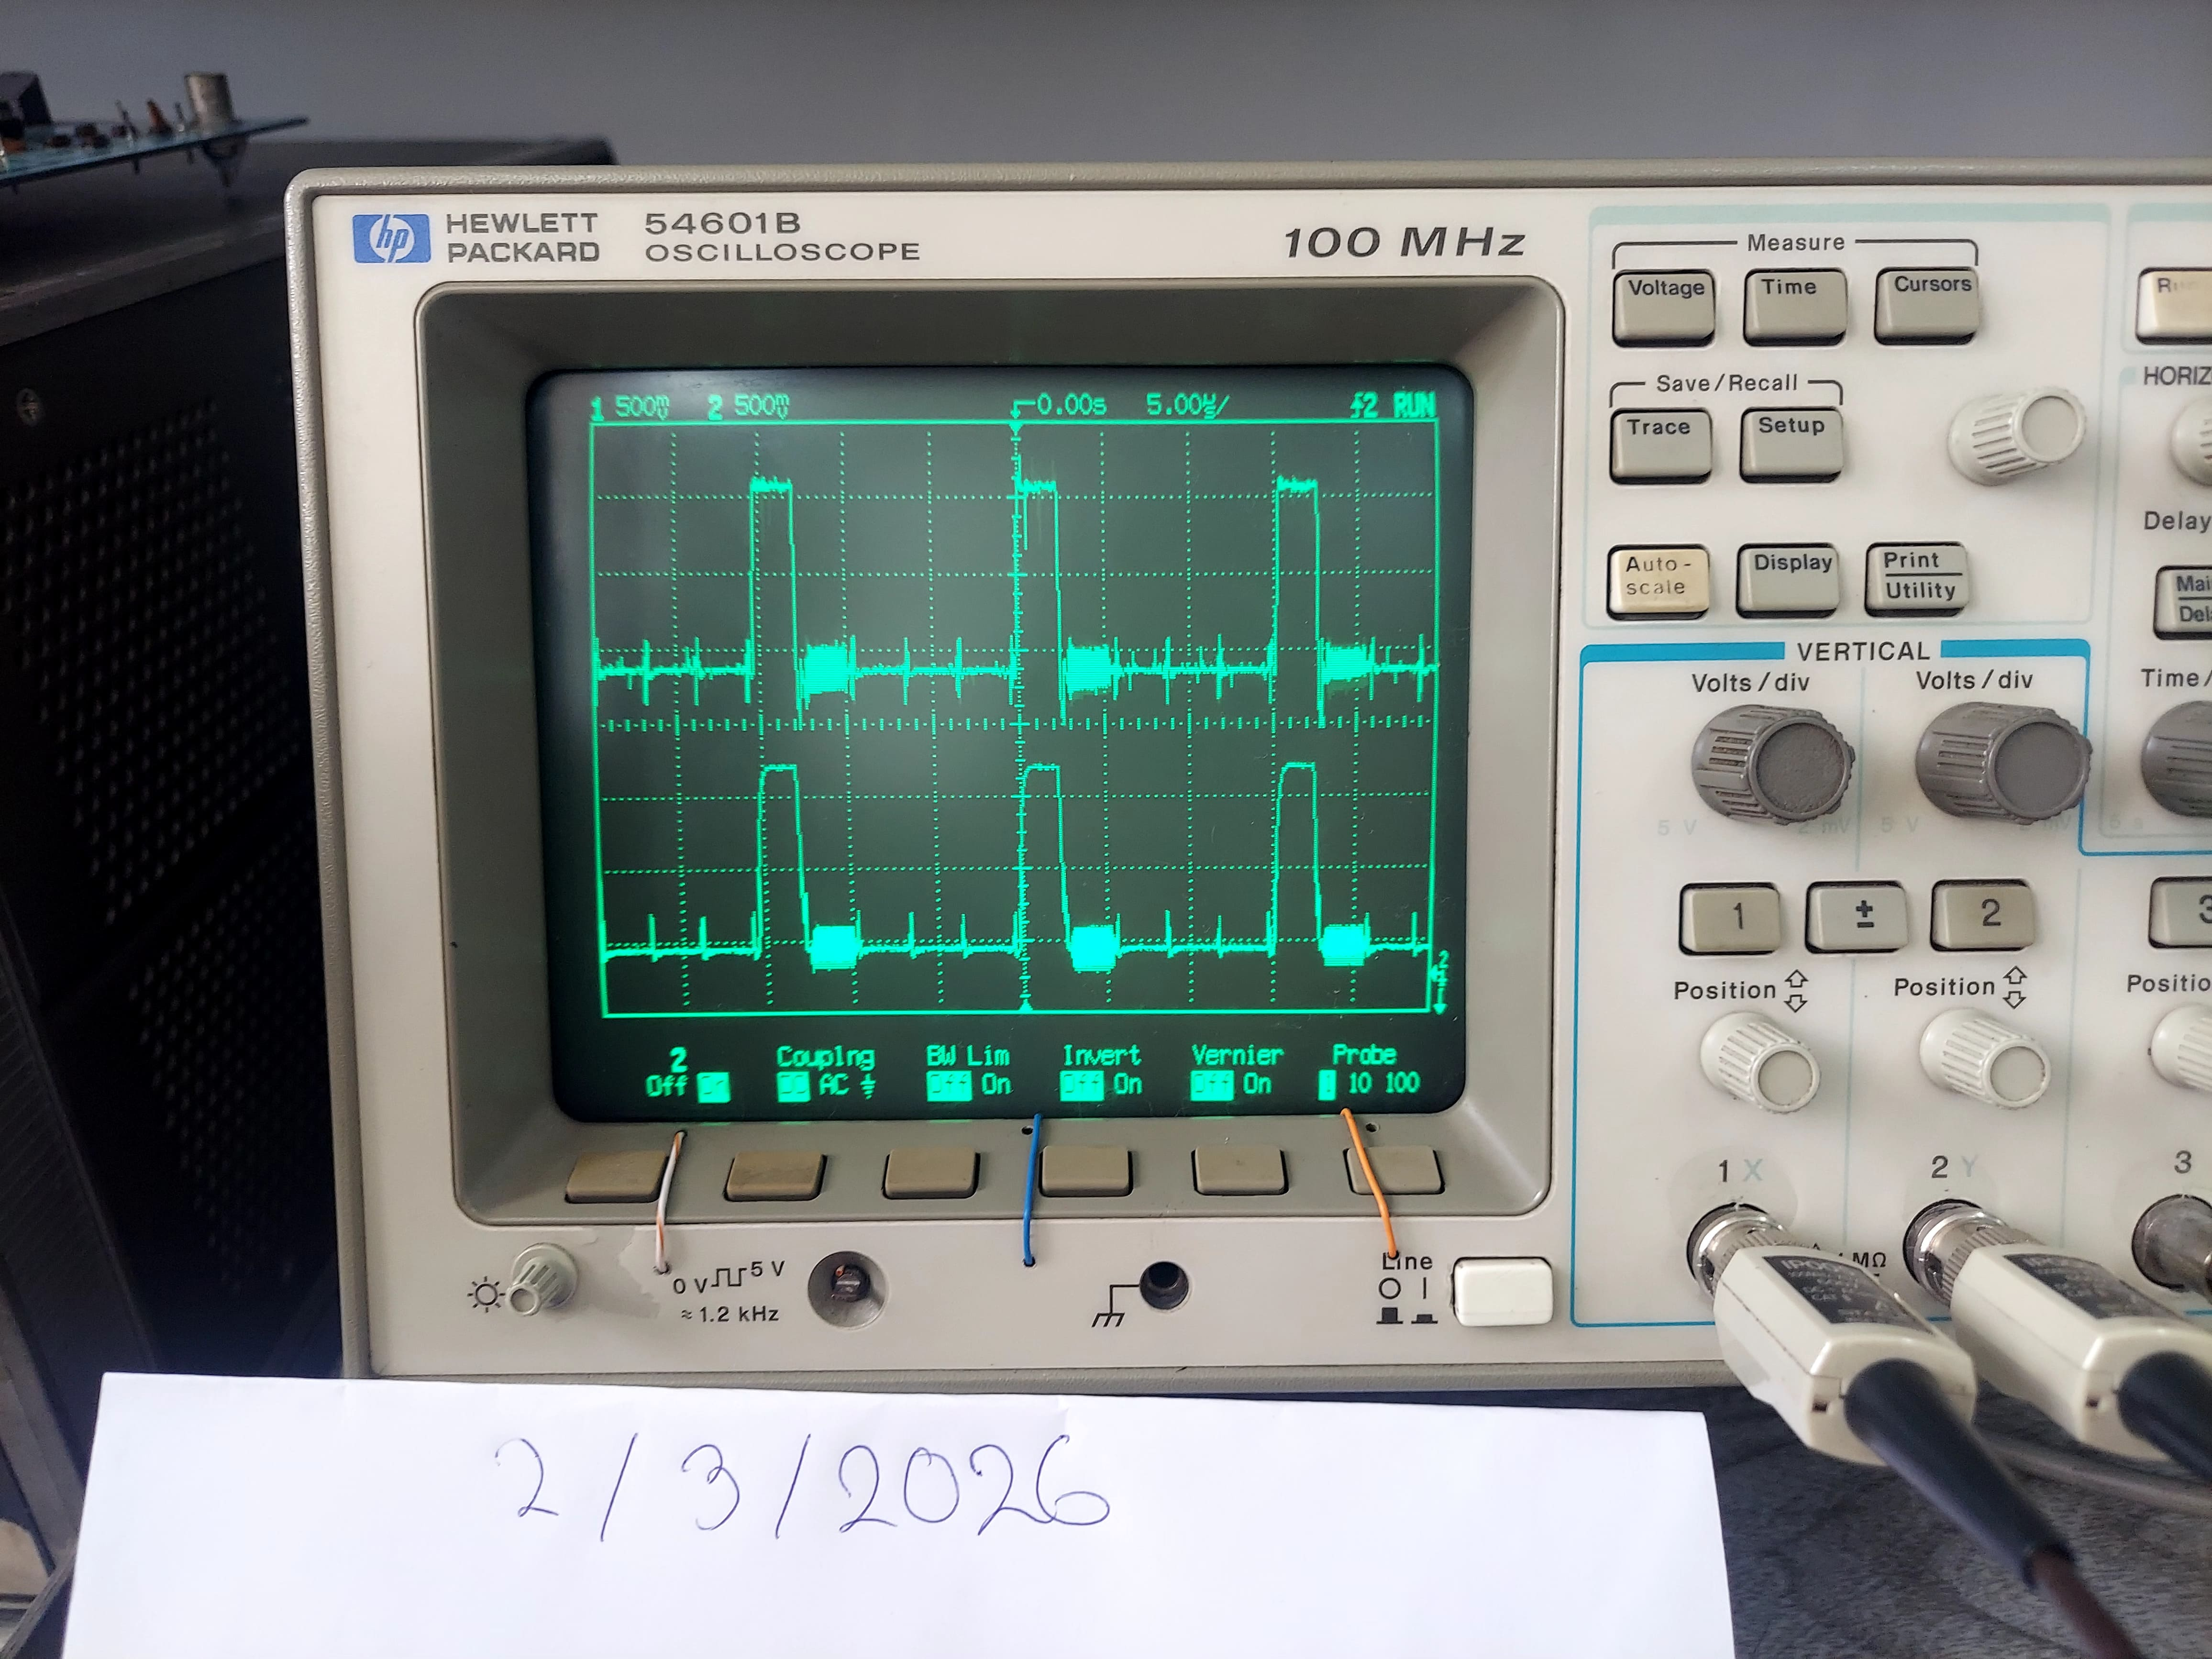
\includegraphics[width=\textwidth]{Imagenes/9-ajuste-gain-4.jpg}
        \caption{Ajuste 4}
    \end{subfigure}
    \\[2ex]
    \begin{subfigure}[b]{0.45\textwidth}
        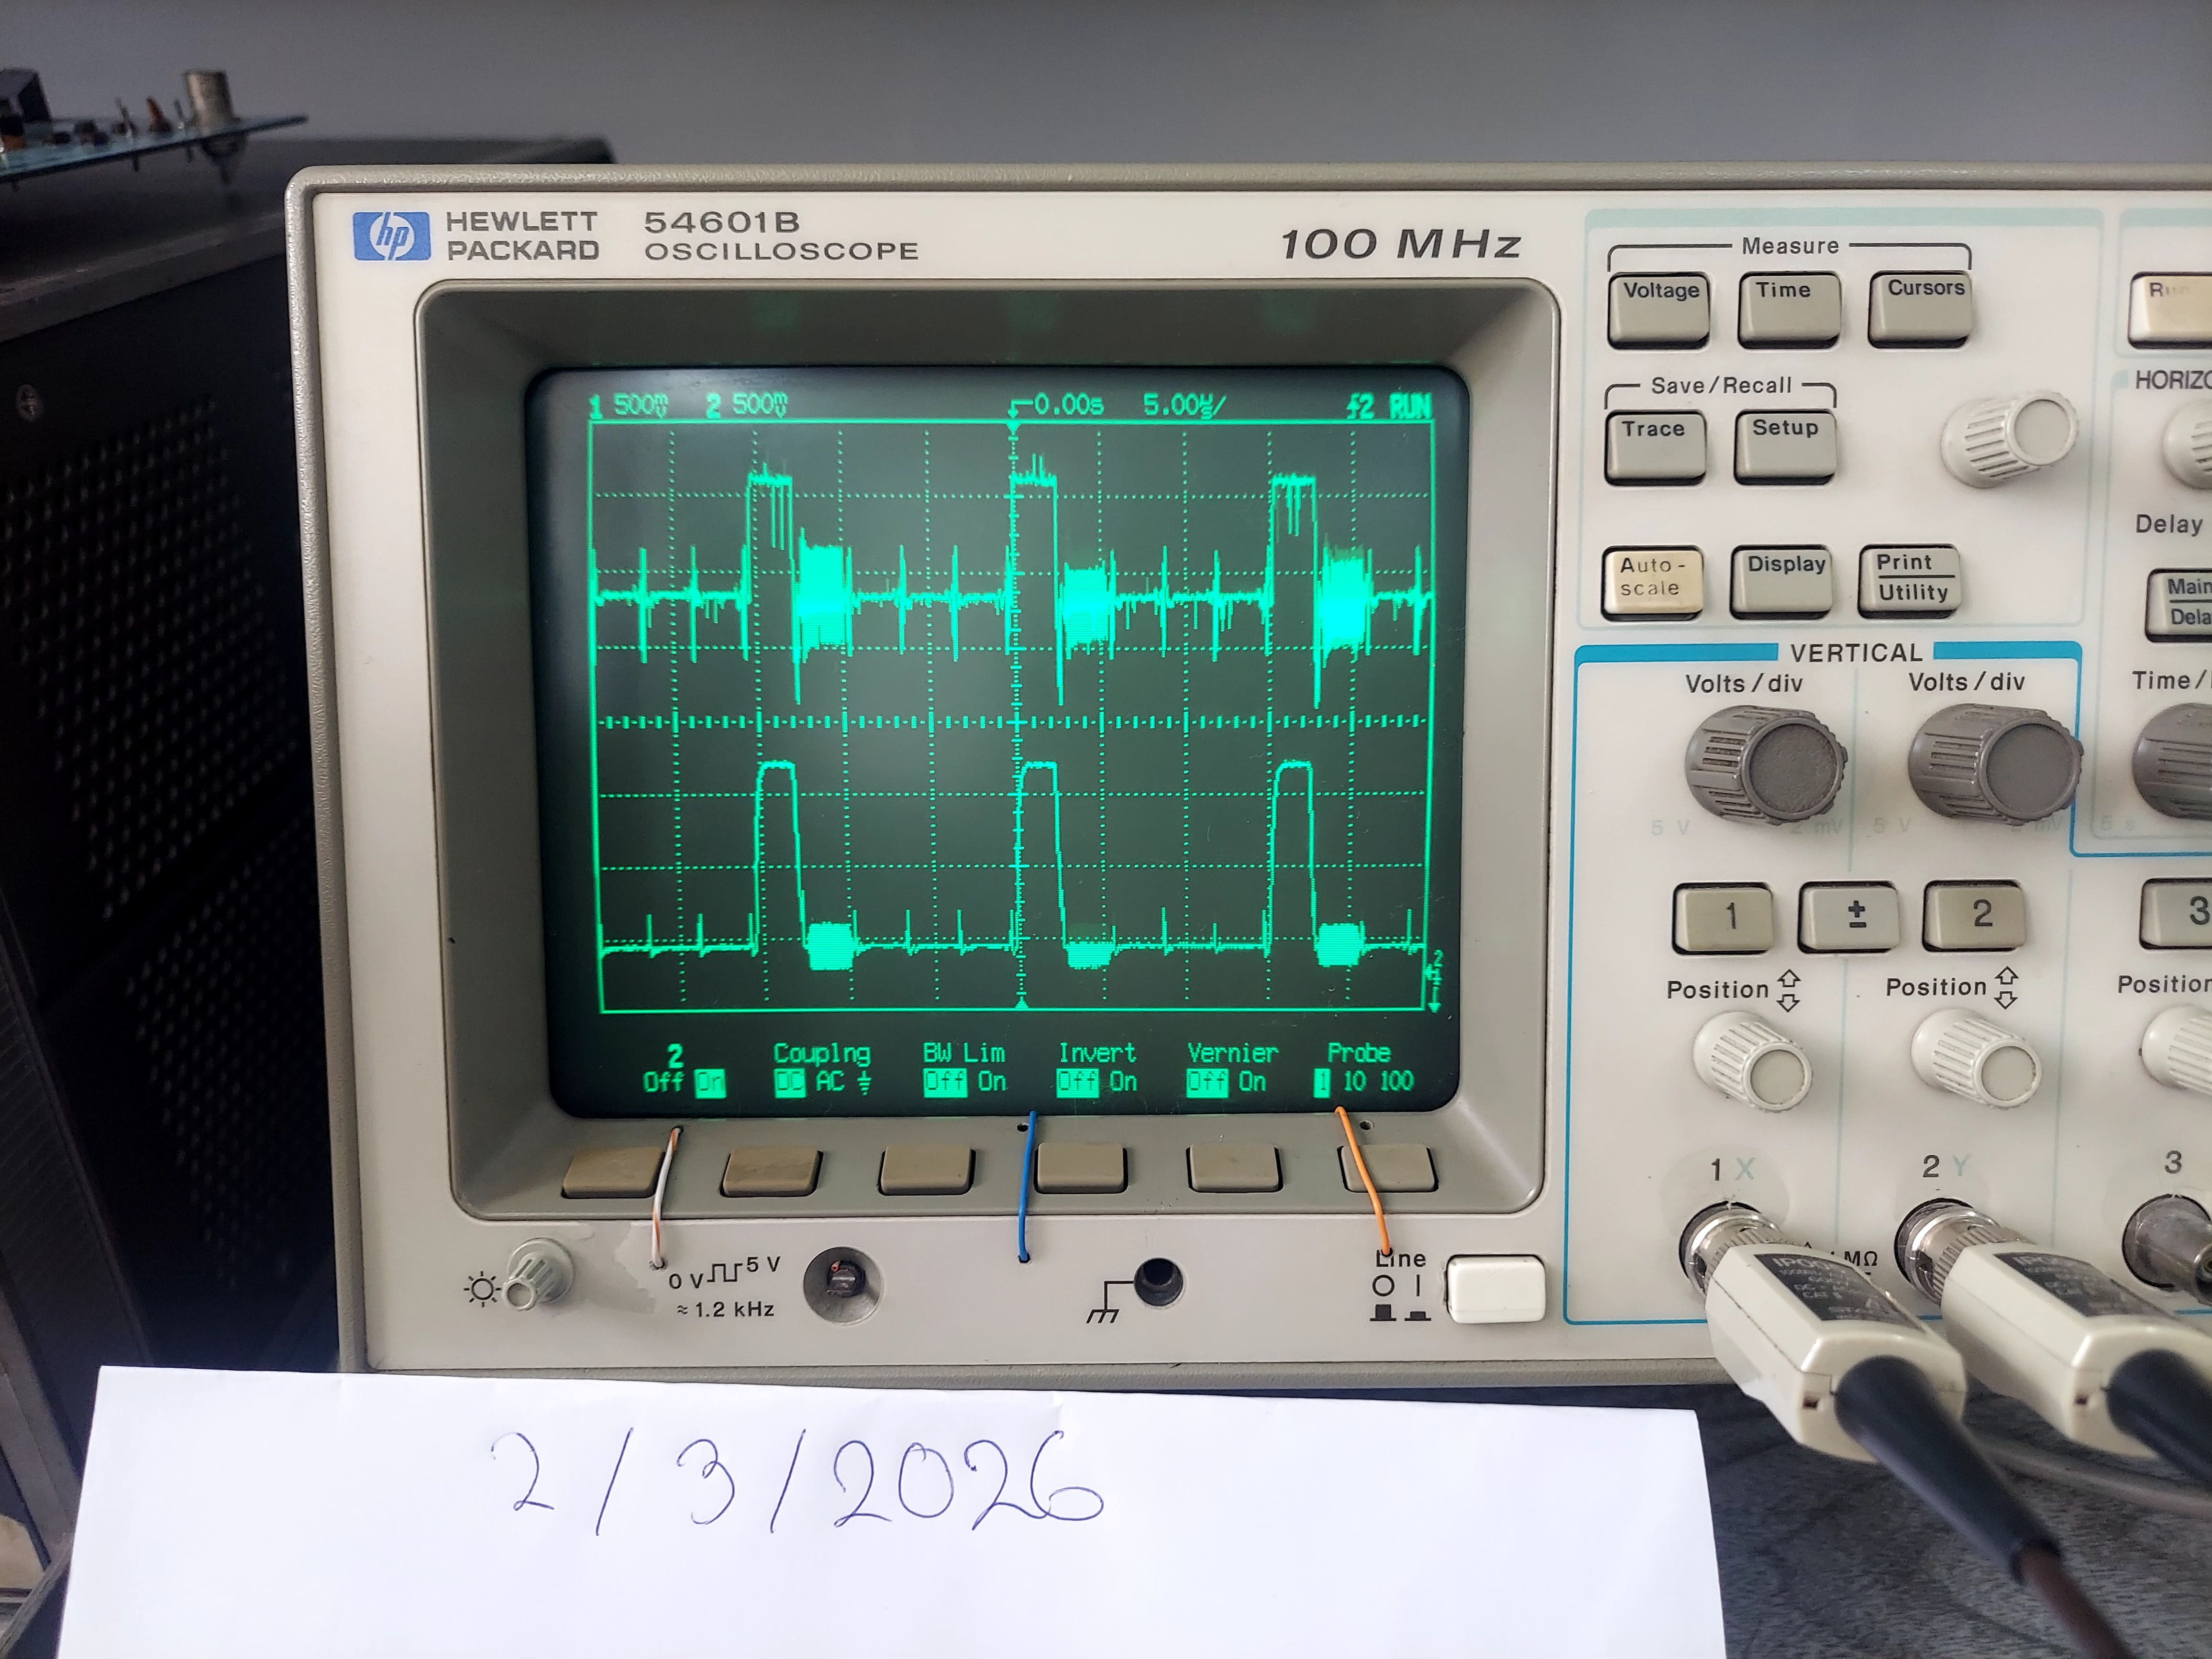
\includegraphics[width=\textwidth]{Imagenes/9-ajuste-gain-5.jpg}
        \caption{Ajuste 5}
    \end{subfigure}
    \hfill
    \begin{subfigure}[b]{0.45\textwidth}
        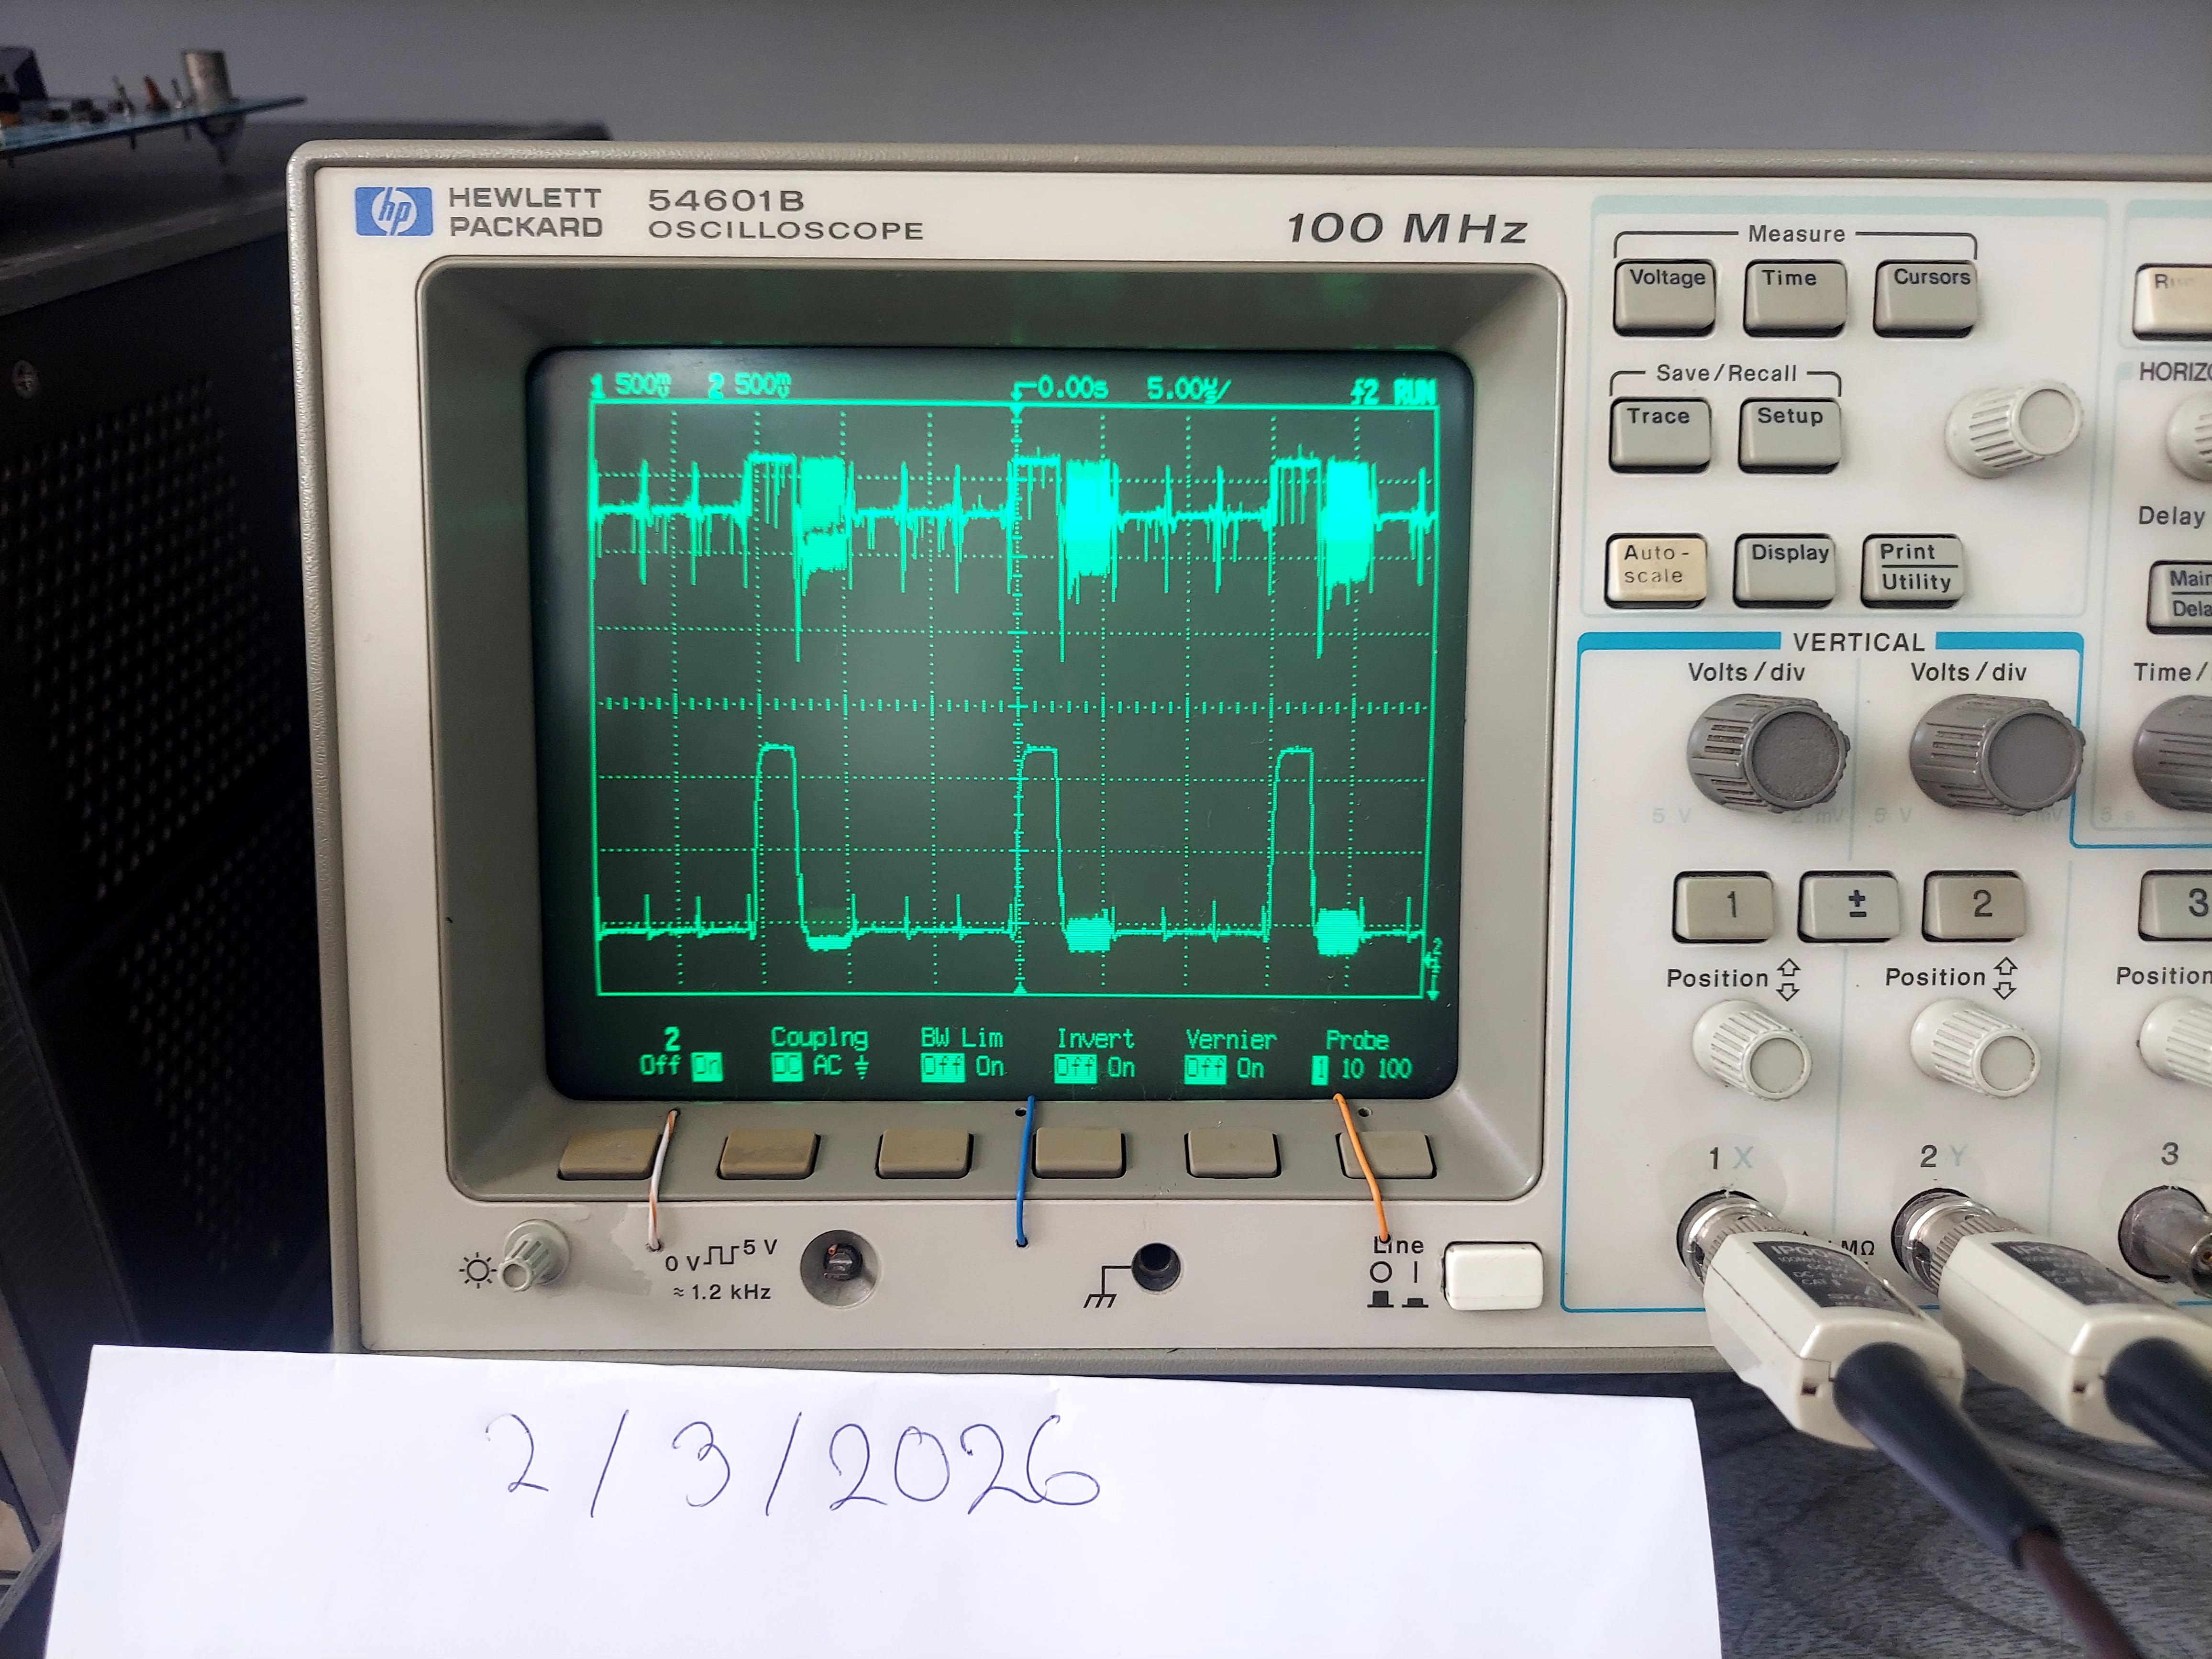
\includegraphics[width=\textwidth]{Imagenes/9-ajuste-gain-6.jpg}
        \caption{Ajuste 6}
    \end{subfigure}
    \\[2ex]
    \begin{subfigure}[b]{0.45\textwidth}
        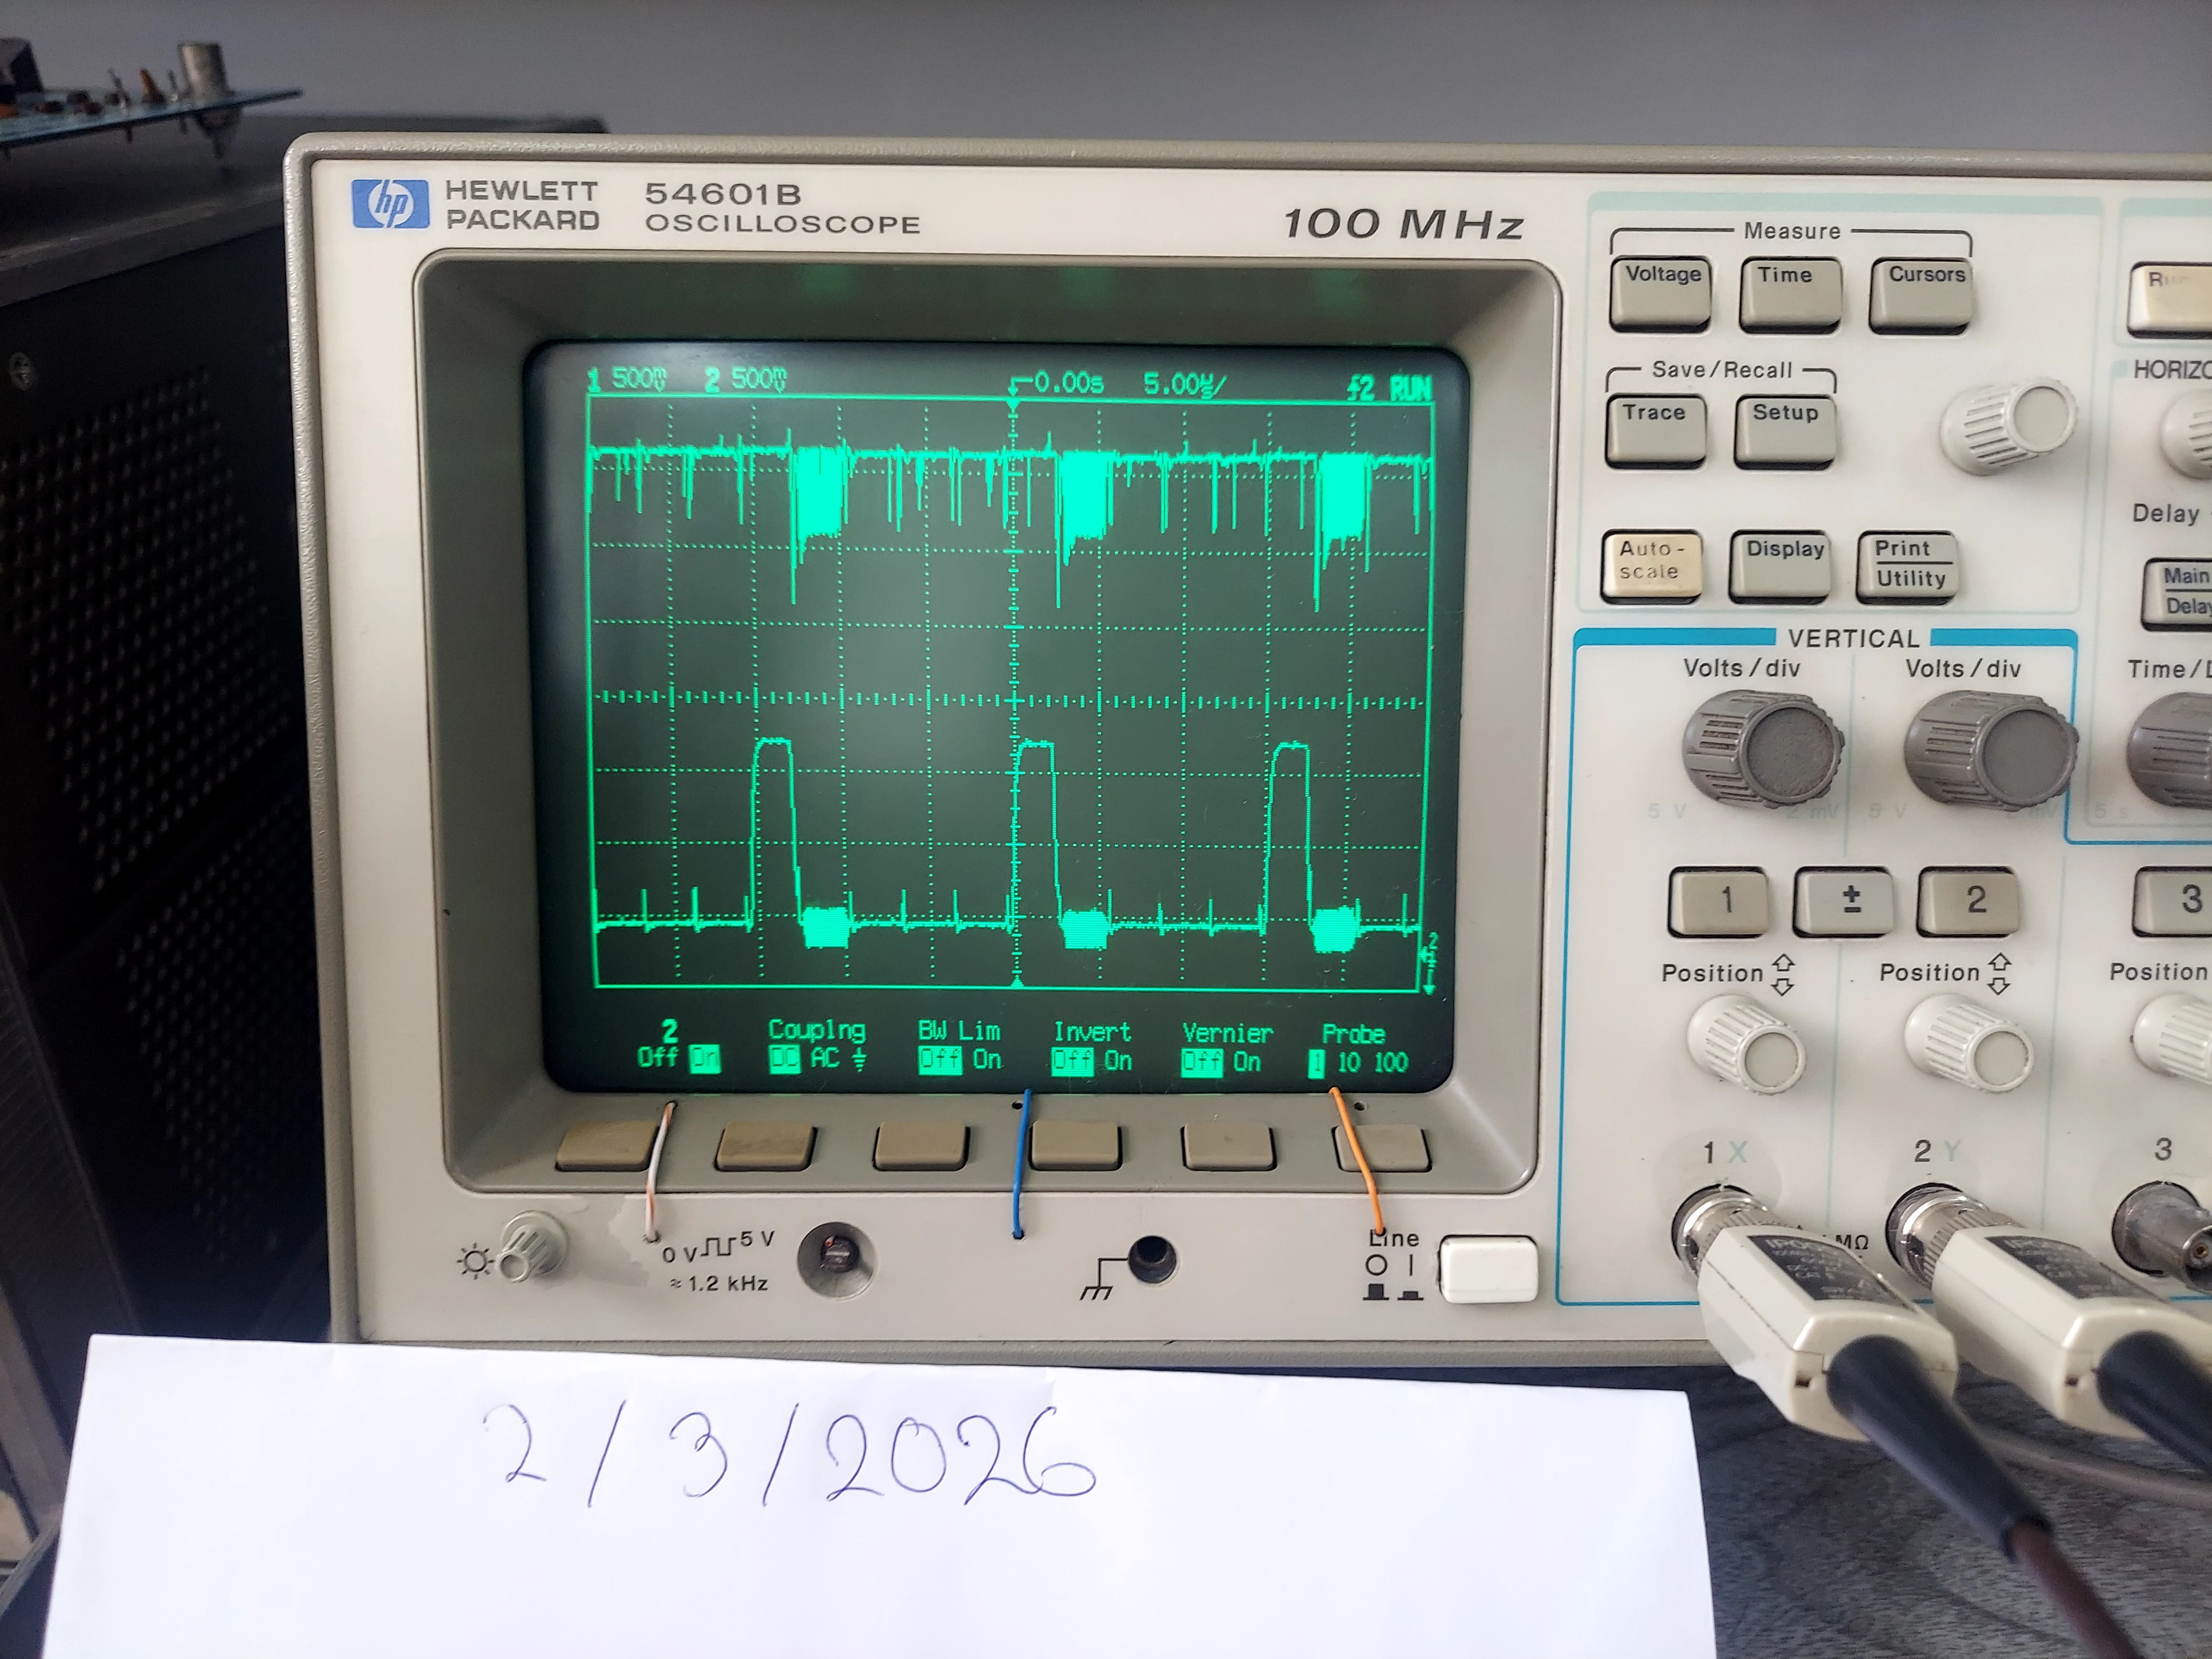
\includegraphics[width=\textwidth]{Imagenes/9-ajuste-gain-7.jpg}
        \caption{Ajuste 7}
    \end{subfigure}
    \caption{Efectos de la variación de GAIN ADJ en la recepción por fibra óptica.}
\end{figure}

\end{document}
